\documentclass[a4j]{ujarticle}
\usepackage[dvipdfmx]{graphicx}
\usepackage{url}
\usepackage{bbding}
\usepackage{lscape}
\usepackage[subrefformat=parens]{subcaption}
\usepackage{bm}
\usepackage{amsmath}
\usepackage{ascmac}
\usepackage{comment}
\usepackage{ascmac}
% \usepackage{fancybx}
% \usepackage{minipage}

\title{ミーティング資料}
\author{安達智哉\\to-adachi@ist.osaka-u.ac.jp}
\date{2020年1月15日}

\begin{document}
\maketitle

% \section{CQ研究会}
% \subsection{質疑応答}
%   \begin{itemize}
%     \item  端末1台1台の通信周期は固定か? 端末の通信周期はアプリケーション毎なのか?\\
%     $\rightarrow$ 本評価では、端末の通信周期は固定である。また、シナリオ2ではアプリケーションごとに通信周期が異なることを想定している。
%     \item default bearerやdedicated bearerなどのベアラがあり、一台の端末が複数のベアラを持つこともできるが、それにも提案手法を適用できるか?\\
%     $\rightarrow$ 現在、複数のベアラを使って通信するようなアプリケーションを想定した提案や評価はできていないため、今後の課題である。一方で、そのような複数ベアラを用いた通信は一般的ではないこともあるため、単一ベアラを対象とした手法でも十分であると言える。
%   \end{itemize}
% \subsection{コメント}
%   \begin{itemize}
%     \item Connected inactive はSYN floodingと同じように、メモリへの攻撃になるのかも。\\
%     $\rightarrow$ Idleタイマをリソース需要に応じて変化させることにより、攻撃に被害を抑制できる可能性がある。Idleタイマの動的制御に関しては、今後の課題である。
%     \item プライベートLTEやローカル5Gなど、一般の企業や個人が自前でモバイルネットワークを構築可能な環境が現在開発されている。これらは、限られたサーバ資源の上で動作する必要があるため、提案手法のような、限られたノード資源を効率的に利用する方法の相性が良いかも。
%     \item MMEが処理できるシグナリング数の限界値は実験に基づいて設定したようだけれど、実際にはCPU負荷は変動が大きいので難しい。
%   \end{itemize}
% - 研究会質疑について
% -- ネットワーク側からは周期はわからない、ということは伝えるべきでしたね。
% -- 各端末は1つのベアラ (default ベアラ) だけを設定する、ということは、
%   説明した方がいいですね。提案方式もそれが前提となっているし、評価の
%   設定も。
%
% - DoS攻撃軽減について
% -- いったんアクティブになった端末のタイマは変更できない、という場合に
%   は、防止は難しいですね。(Inactiveになってそのまま黙られると、メモリ
%   使われてしまう) 後続で接続してくる端末に対しては対応できるけど。
% - CPU変動が激しいのは負荷が高い時のようなので、CPU負荷の監視をどうする
%  か、ですね。なので、一般的なサーバのCPU負荷の監視、という話で、探せ
%  ば、方式はあると思う。

\begin{comment}
\section{Idleタイマの制御方法}
\label{sec:hard-state}
本節では、UEの強制的な状態変化を引き起こさないことを前提にする。
つまり、Idleタイマが切れていないUEを強制的にIdle状態へ遷移させることはないとする。
また、Idleタイマの更新は、UEがデータ送信を行うタイミングで実行するものとする。
MMEはUEを収容するために使用されているCPUおよびメモリリソース量を観測できるものとする。
つまり、UEの収容とは無関係な処理によって発生する負荷を取り除いたCPU負荷およびメモリ使用量を知ることができるとする。


突発的な負荷の増加に対応するという観点から、現在収容しているUEに加え、最も多くのUEを収容できるようなIdleタイマの値が最適と考える。
具体的には、現在収容しているUEと同じ通信周期を持つUEがネットワークに参加すると仮定し、収容可能なUE台数が最大となるIdleタイマの値を最適と定義する。
また、CPUおよびメモリのどちらも過負荷状態でないことは、UEを収容可能であることの必要十分条件であるとする。

まず、現在収容しているUE台数を$N_{\rm UE}$とする。
UE台数が$N_{\rm UE}$、Idleタイマが$T$の時に観測される、CPUおよびメモリの使用量をそれぞれ$C_{N_{\rm UE}}(T)$、$M_{N_{\rm UE}}(T)$とする。

Idleタイマを$T$とした時に、収容可能なUEの総数を$N_{\rm UE}^{\rm capa}(T)$とすると$N_{\rm UE}^{\rm capa}(T)$は、$C_{N_{\rm UE}}(T)$、$M_{N_{\rm UE}}(T)$、$C^{\rm max}$および$M^{\rm max}$を用いて、以下の式(\ref{eq:UE_add})で表せる。
ここで、$C^{\rm max}$、$M^{\rm max}$はそれぞれシグナリング処理およびUEのセッション情報を保持するために使用可能なCPUリソース量およびメモリリソース量である。
\begin{eqnarray}
   N_{\rm UE}^{\rm capa}(T) =& \lfloor N_{\rm UE} \cdot \min \{\frac{C^{\rm max}}{C_{N_{\rm UE}}(T)}, \frac{M^{\rm max}}{M_{N_{\rm UE}}(T)}\} \rfloor\label{eq:UE_add}
\end{eqnarray}
Idleタイマを制御する上での目的関数を以下の式(\ref{eq:objective_function})に示す。
\begin{eqnarray}
  \text{maximize} :& N_{\rm UE}^{\rm capa}(T)
  \label{eq:objective_function}
\end{eqnarray}

$N_{\rm UE}^{\rm capa}(T)$を最大化するIdleタイマの値が明らかである場合は、その値をIdleタイマに設定すれば良い。
しかし一般的に、UEの台数や通信周期は未知であり時間的に変動するため、$N_{\rm UE}^{\rm capa}(T)$を最大化するIdleタイマの値を知ることは難しい。
そのような場合は、$N_{\rm UE}^{\rm capa}(T)$を最大化するように、Idleタイマを適応的に制御する必要がある。
具体的には、各リソースの使用量を観測して、$N_{\rm UE}^{\rm capa}(T)$を大きくする向きにIdleタイマを変化させる。
このステップを複数回繰り返すことにより、Idleタイマを制御する。

この時、1ステップごとのIdleタイマの変化量を考える必要がある。
この値を小さく設定すると、最適な値に到達するまでに大きな時間がかかってしまう場合がある。
逆にIdleタイマの変化量を大きく設定すると、Idleタイマが発振する可能性もあり、制御が不安定になる。
また、UEの通信周期によって、Idleタイマが変化した時に各リソースの負荷の変化量が異なる点も考慮する必要がある。
つまり、ネットワークの変化に短い時間スケールで対応しつつ、安定した制御を実現するためには、ネットワークの環境に応じてIdleタイマの変化量を制御する仕組みが必要である。
このような制御には様々な手法が考えられるが、本報告では動作がシンプルであり、汎用性が高いPID制御を用いる。


まず、PID制御における出力値$y(t)$および目標値$r(t)$を設定する。
以前の評価より、CPU使用量はIdleタイマの値に対して広義単調減少でありかつ、メモリ使用量はIdleタイマの値に対して広義単調増加であることがわかっている。
このことから、式(\ref{eq:UE_add})を確認すると、$\frac{C^{\rm max}}{C_{N_{\rm UE}}(T)}$は広義単調増加でありかつ、$\frac{M^{\rm max}}{M_{N_{\rm UE}}(T)}$は広義単調減少であることがわかる。
ここで、以下の式(\ref{eq:c=m})を満たすような$T$の集合を$\bm{T}$とし、$N_{\rm UE}^{\rm capa}(T)$を最大化するような$T$の集合を$\bm{T}_{\rm optimal}$とすると、$T\in\bm{T}$であることは$T\in\bm{T}_{\rm optimal}$であるための十分条件になる。
\begin{eqnarray}
\frac{C^{\rm max}}{C_{N_{\rm UE}}(T)}=\frac{M^{\rm max}}{M_{N_{\rm UE}}(T)}
  \label{eq:c=m}
\end{eqnarray}


以上の議論のイメージを図\ref{theory_1_all_30s_theory}、図\ref{theory_1_add_C_M}および図\ref{theory_1_add_all}に示す。
図\ref{theory_1_all_30s_theory}はUE台数が500,000台,UEごとの通信周期は10~sから6,000~sの範囲で一様分布とした時の、Idleタイマと各リソース負荷の関係を示したものである。
図\ref{theory_1_add_C_M}は図\ref{theory_1_all_30s_theory}と同じUEを収容した時の、Idleタイマと$N_{\rm UE} \cdot \frac{C^{\rm max}}{C_{N_{\rm UE}}(T)}$と$N_{\rm UE} \cdot \frac{M^{\rm max}}{M_{N_{\rm UE}}(T)}$との関係を示している。
また、図\ref{theory_1_add_all}は図\ref{theory_1_all_30s_theory}と同じUEを収容した時の、Idleタイマと$N_{\rm UE}^{\rm capa}(T)$との関係を示している。
図\ref{theory_1_add_all}を見ると、$N_{\rm UE}^{\rm capa}(T)$を最大化するIdleタイマの値と$\frac{C^{\rm max}}{C_{N_{\rm UE}}(T)}=\frac{M^{\rm max}}{M_{N_{\rm UE}}(T)}$となる時のIdleタイマの値が一致していることが確認できる。

\begin{figure}[htbp]
  \centering
  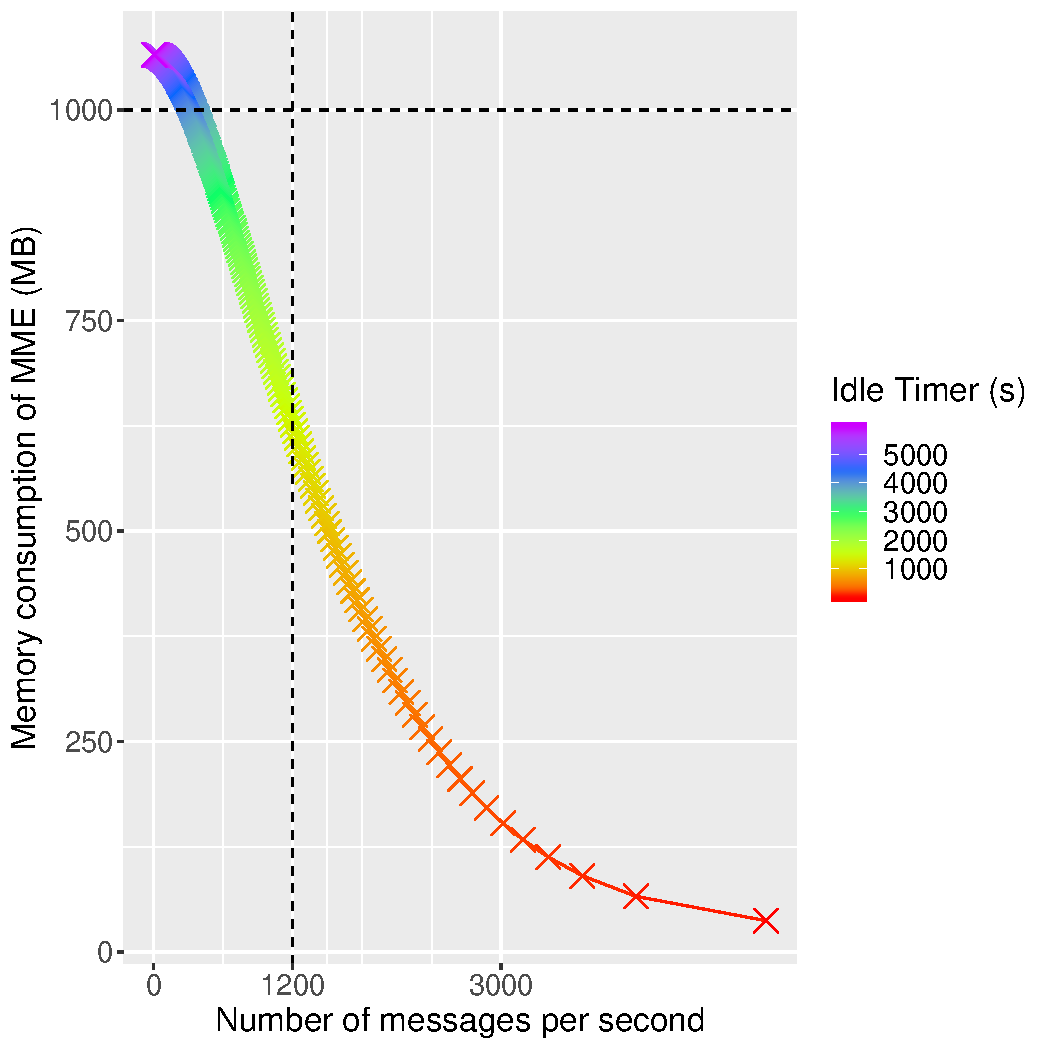
\includegraphics[width=0.5\hsize]{theory_1_all_30s_theory.pdf}
  \caption{Idleタイマに対する,メッセージ処理頻度とメモリ使用量の関係}
  \label{theory_1_all_30s_theory}
\end{figure}


\begin{figure}[htbp]
 \centering
 \begin{subfigure}{0.49\hsize}
   \centering
   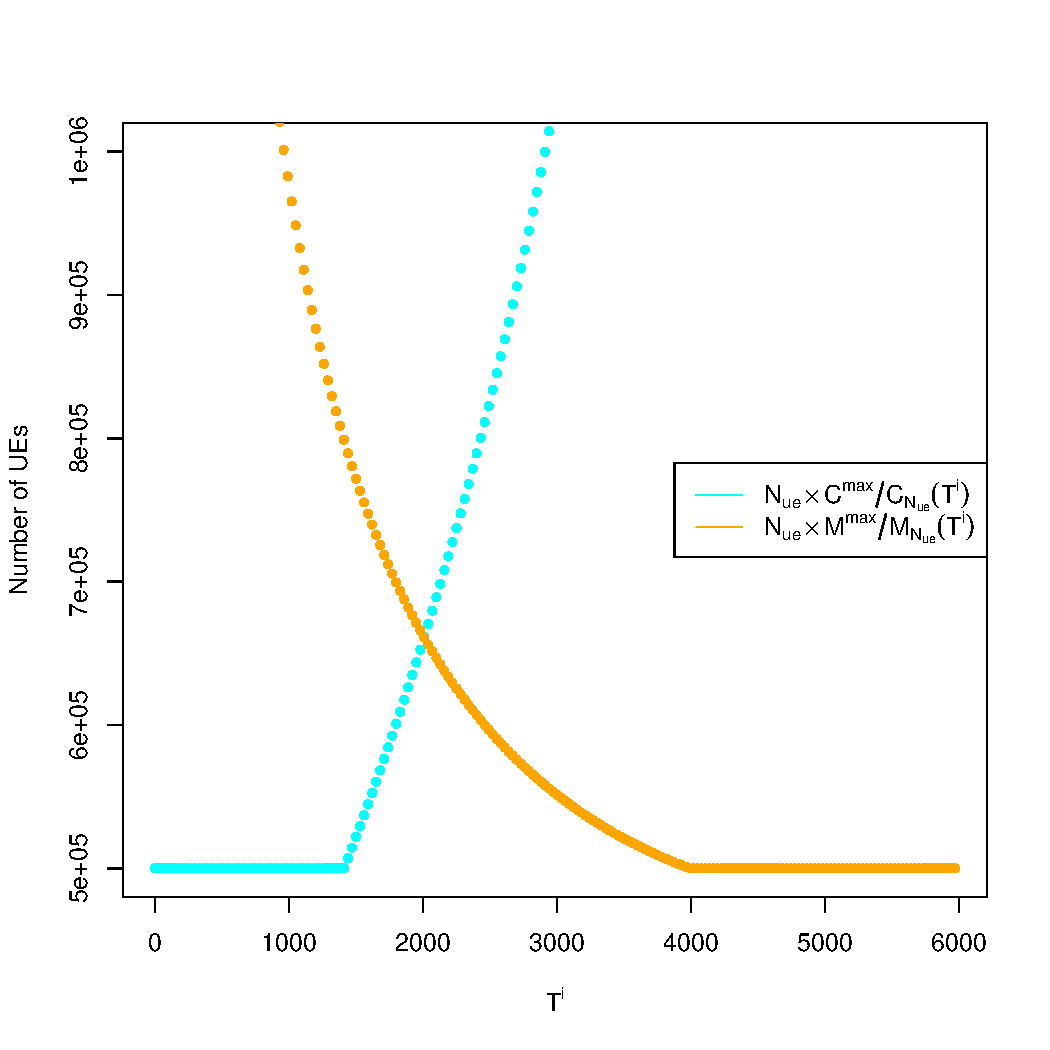
\includegraphics[width=1\hsize]{theory_1_add_C_M.pdf}
   \subcaption{Idleタイマと$N_{\rm UE} \cdot \frac{C^{\rm max}}{C_{N_{\rm UE}}(T)}$と$N_{\rm UE} \cdot \frac{M^{\rm max}}{M_{N_{\rm UE}}(T)}$の関係}
   \label{theory_1_add_C_M}
 \end{subfigure}
 \begin{subfigure}{0.49\hsize}
   \centering
   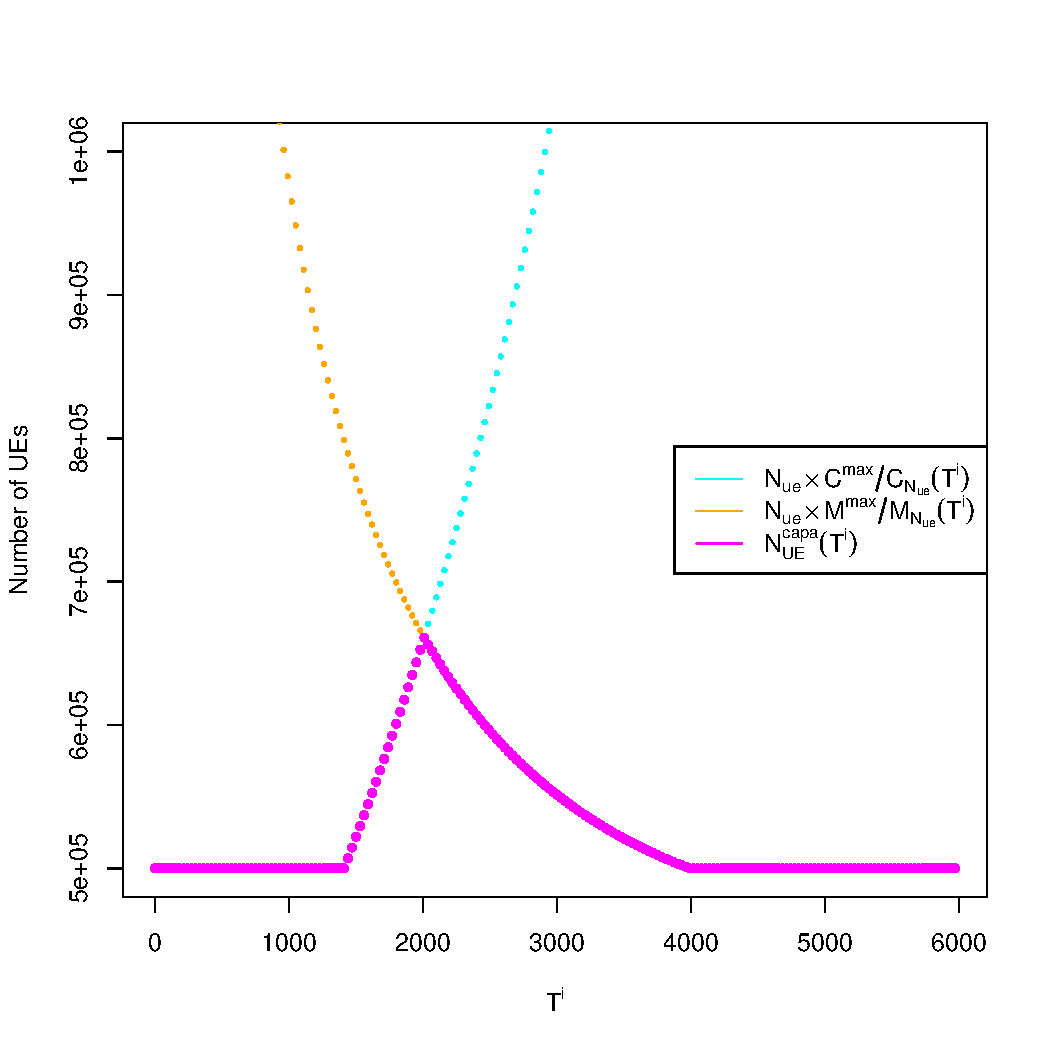
\includegraphics[width=1\hsize]{theory_1_add_all.pdf}
   \subcaption{Idleタイマと$N_{\rm UE}^{\rm capa}(T)$の関係}
   \label{theory_1_add_all}
 \end{subfigure}
 \caption{}
 \label{}
\end{figure}

式(\ref{eq:c=m})は分母と分子を入れ替えても成り立つことを考慮し、PID制御における出力値$y(t)$および目標値$r(t)$を以下の式(\ref{eq:PID_y_t})、(\ref{eq:PID_r_t})のように定義する。
$t$は時刻を表す変数である。
\begin{eqnarray}
  y(t) &=& \frac{C_{N_{\rm UE}}(T)}{C^{\rm max}} - \frac{M_{N_{\rm UE}}(T)}{M^{\rm max}}
  \label{eq:PID_y_t} \\
  r(t) &=& 0
  \label{eq:PID_r_t}
\end{eqnarray}

時刻$t$における$y(t)$と$r(t)$の差を$e(t)$として以下の式(\ref{eq:PID_e_t})ように定義すると、PID制御における操作量($u(t)$)は以下の式(\ref{eq:PID_u_t})で表せる。
\begin{eqnarray}
  e(t) &=& r(t) - y(t)
  \label{eq:PID_e_t} \\
  u(t) &=& K_p \cdot e(t) + K_i \cdot \int_0^t e(\tau) d\tau + K_d \cdot \frac{de(t)}{dt}
  \label{eq:PID_u_t}
\end{eqnarray}
ここで、$K_p$、$K_i$および$K_d$はそれそれ、比例ゲイン、積分ゲインおよび微分ゲインと呼ばれる定数である。
これらの定数は、$e(t)$およびその積分値、微分値が$u(t)$にどの程度寄与するのかを決定する。




\section{ジーグラニコルスの限界感度法}
\label{gigura}
PID制御においては、比例ゲイン($K_p$)、積分ゲイン($K_i$)、微分ゲイン($K_d$)と呼ばれる3つの定数を設定する必要がある。これらの定数を``ジーグラ・ニコルスの限界感度法"と呼ばれる手順に基づき設定した。

ジーグラ・ニコルスの限界感度法に基づくゲインの求め方を以下に示す。
\begin{description}
  \item[ステップ~1] 積分ゲイン($K_i$)および微分ゲイン($K_d$)を0にして調節器が比例動作だけを行うようにする。
  \item[ステップ~2] 比例ゲイン($K_p$)を0から徐々に大きくしていき、制御量が安定限界に達して一定振幅振動を持続するようになった時に$K_p$の増加を止める。
  \item[ステップ~3] ステップ~2の時の比例ゲインを限界感度($K_u$)、振動周期を限界周期($P_u$)とし、これらの値から各ゲインを以下の表\ref{table:Ziegler-Nichols}のように求める。
  \item[ステップ~4]必要に応じてステップ~3で求めた各ゲインの値を調整する。
\end{description}
\begin{table}[]
  \centering
  \caption{ジーグラ・ニコルスの限界感度法}
  \label{table:Ziegler-Nichols}
  \begin{tabular}{c|c|c|c|c|c}
    \hline
    制御の種類  & $K_p$ & $K_i$ & $K_d$ & $T_i$ & $T_d$ \\\hline \hline
    P & 0.5$K_u$ & 0 & 0 & - & - \\
    PI & 0.45$K_u$ & $K_p/0.83P_u$ & 0 & $0.83P_u$ & - \\
    PID & 0.6$K_u$ & $K_p/0.5P_u$  & $K_p \cdot 0.125P_u$ & $0.5P_u$ & $0.125P_u$ \\\hline
  \end{tabular}
\end{table}

以下のシナリオにおいて、ジーグラニコルスの限界感度法を用いて、PID制御のゲインを求めた。
UE台数は648,000台であり、UEの持つ通信周期は1~day,2~hours,1~hour,30~minutesのいずれかである。それぞれの通信周期を持つUEの割合は表\ref{table:interval}の通りである。また、各パラメータを表\ref{table:parameter}に示す。
\begin{table}[htbp]
  \centering
  \caption{パラメータ設定}
  \label{table:parameter}
  \begin{tabular}{c|l}
    \hline
    Parameter  & Numerical setting \\\hline \hline
    $T^{\rm ci}$ & 10~s\\
    $s_{\rm MME}^{\rm c \to \rm c}$ & 0~messages\\
    $s_{\rm MME}^{\rm ci \to \rm ci}$ & 0~messages\\
    $s_{\rm MME}^{\rm c \to \rm ci}$ & 0~messages\\
    $s_{\rm MME}^{\rm ci \to \rm c}$ & 0~messages\\
    $s_{\rm MME}^{\rm ci \to \rm i}$ & 5~messages\\
    $s_{\rm MME}^{\rm i \to \rm c}$ & 5~messages\\
    $m^{\rm c}_{\rm MME}$ & 17878~bits\\
    $m^{\rm ci}_{\rm MME}$ & 17878~bits\\
    $m^{\rm i}_{\rm MME}$ & 408~bits\\
    $C^{\rm max}$ & 1200~messages/s\\
    $M^{\rm max}$ & 1,000~MB\\
    $d_h$ & 1 \\\hline
  \end{tabular}
\end{table}
\begin{table}[htbp]
  \centering
  \caption{UEの通信周期の分布}
  \label{table:interval}
  \begin{tabular}{c|cccc}
    \hline
    &\multicolumn{4}{c}{通信周期} \\
    & 1~day & 2~hours & 1~hour & 30~minutes \\\hline \hline
    UE台数の割合 & 40\% & 40\% & 15\% & 5\% \\\hline
  \end{tabular}
\end{table}


まず、限界感度および限界周期を求めるために、$K_i$および$K_d$を0にして、$K_p$を0から徐々に大きくしていった。
その結果を図\ref{fig:result_1}、図\ref{fig:result_2}、図\ref{fig:result_3}および図\ref{fig:result_4}に示す。
これらの図は$K_p=1$、$K_p=2$、$K_p=2.875$、$K_p=3$の場合の結果を示している。
これらの図を見ると、$K_p=2.875$以下の場合は制御が収束するが、$K_p=3$の場合は制御が収束せず、一定振幅振動していることがわかる。
このことから、限界感度($K_u$)を3とする。
また、限界周期($P_u$)は図\ref{fig:result_4}より、8000~sとする。
\begin{figure}[htbp]
 \centering
 \begin{subfigure}{0.49\hsize}
   \centering
   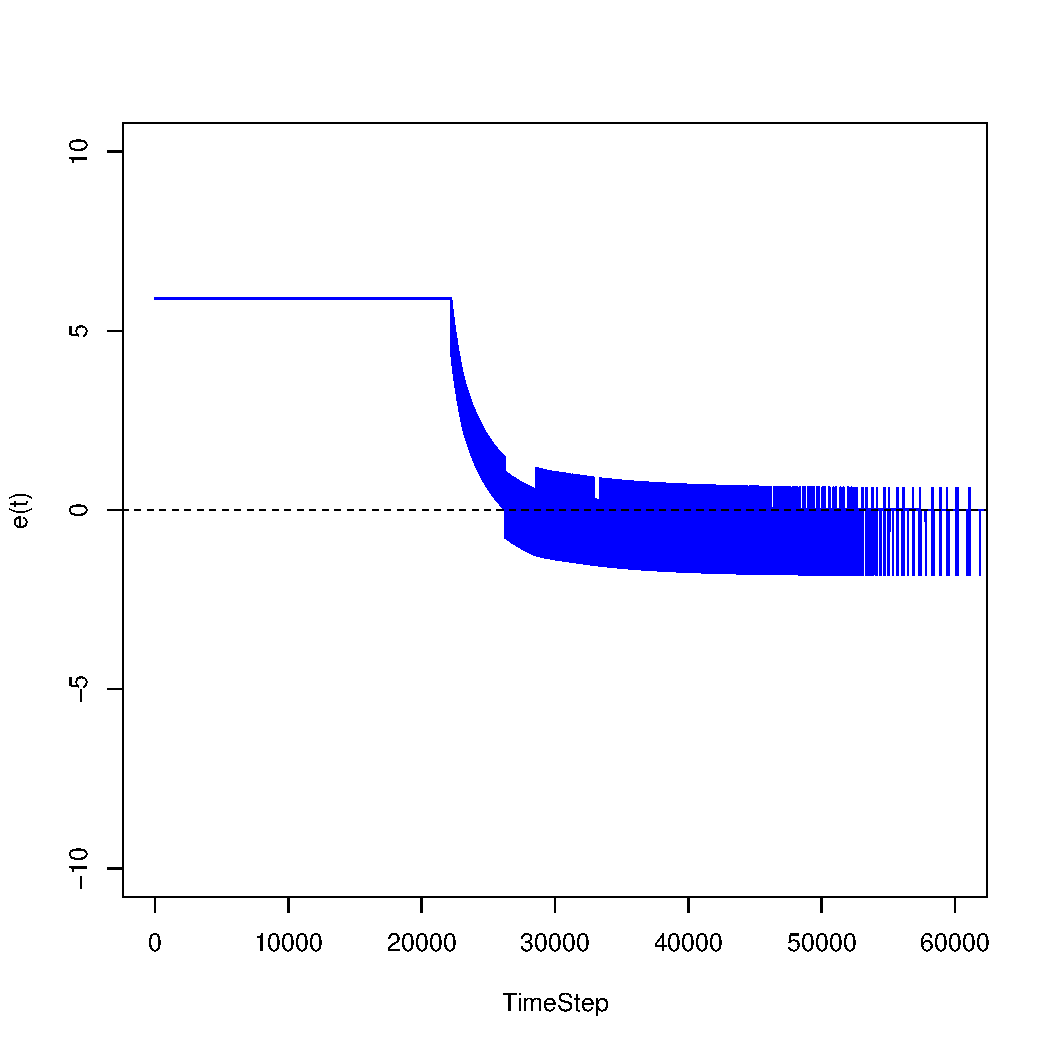
\includegraphics[width=1.0\hsize]{scenario_5_e_86400_345600_1_0_0_0_ideal.pdf}
   \subcaption{$e(t)$の変化}
   \label{subfig:scenario_5_e_86400_345600_0-318_1_0_0_0_ideal}
 \end{subfigure}
 \begin{subfigure}{0.49\hsize}
   \centering
   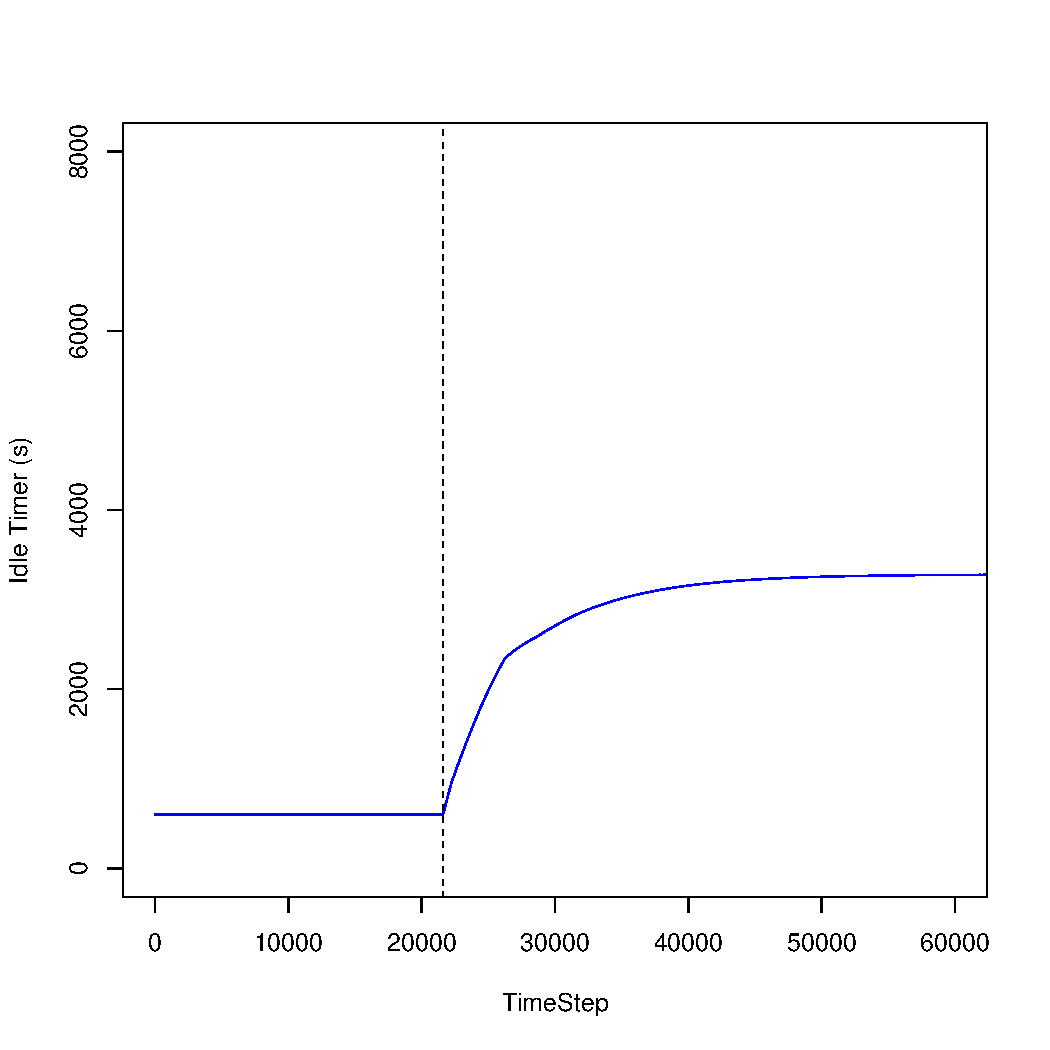
\includegraphics[width=1.0\hsize]{scenario_5_idleTimer_86400_345600_1_0_0_0_ideal.pdf}
   \subcaption{IdleTimerの変化}
   \label{subfig:scenario_5_idleTimer_86400_345600_1_0_0_0_ideal}
 \end{subfigure}
 \par\bigskip %改行
 \begin{subfigure}{0.49\hsize}
   \centering
   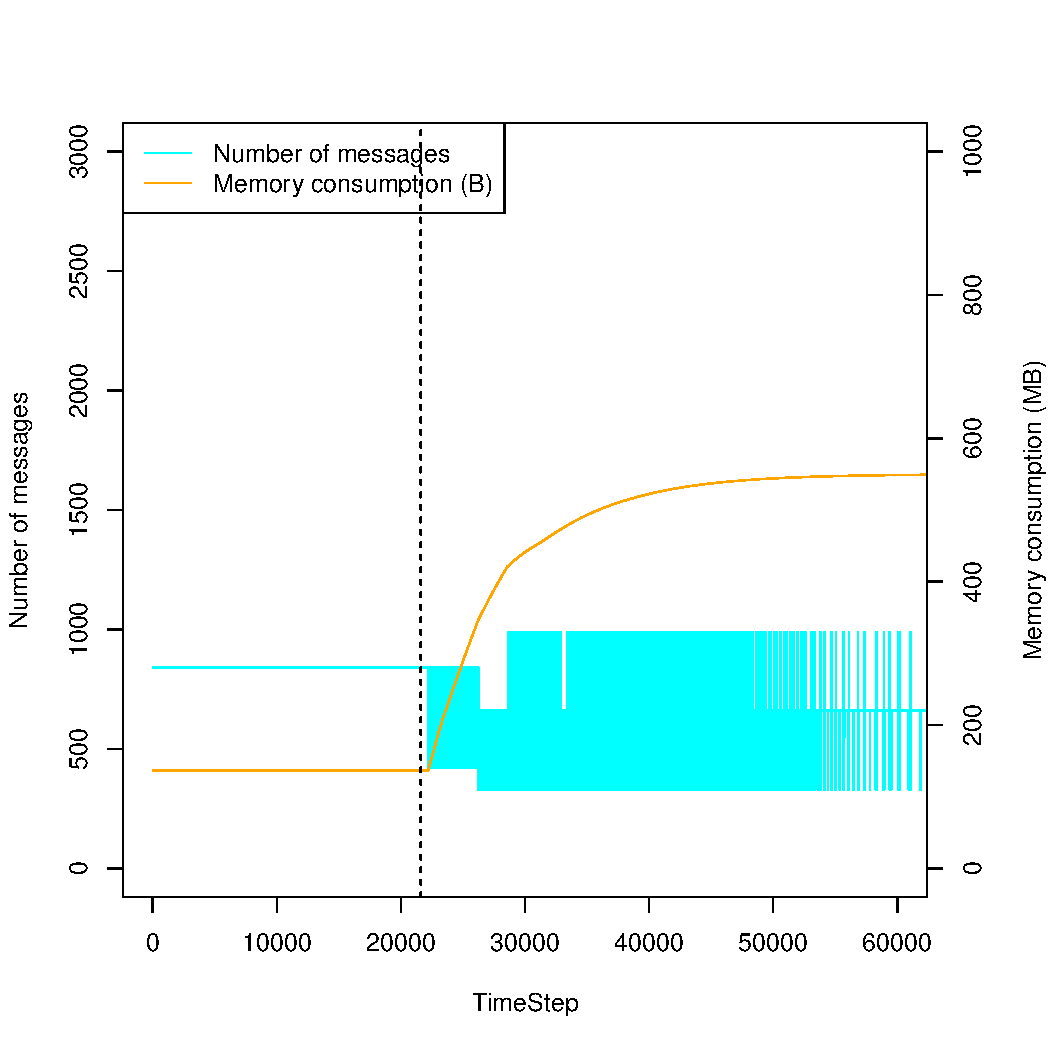
\includegraphics[width=1.0\hsize]{scenario_5_signaling_and_memoryload_vs_timeStep_86400_345600_1_0_0_0_ideal.pdf}
   \subcaption{CPU負荷とメモリ使用量の変化}
   \label{subfig:scenario_5_signaling_and_memoryload_vs_timeStep_86400_345600_1_0_0_0_ideal}
 \end{subfigure}
 \begin{subfigure}{0.49\hsize}
   \centering
   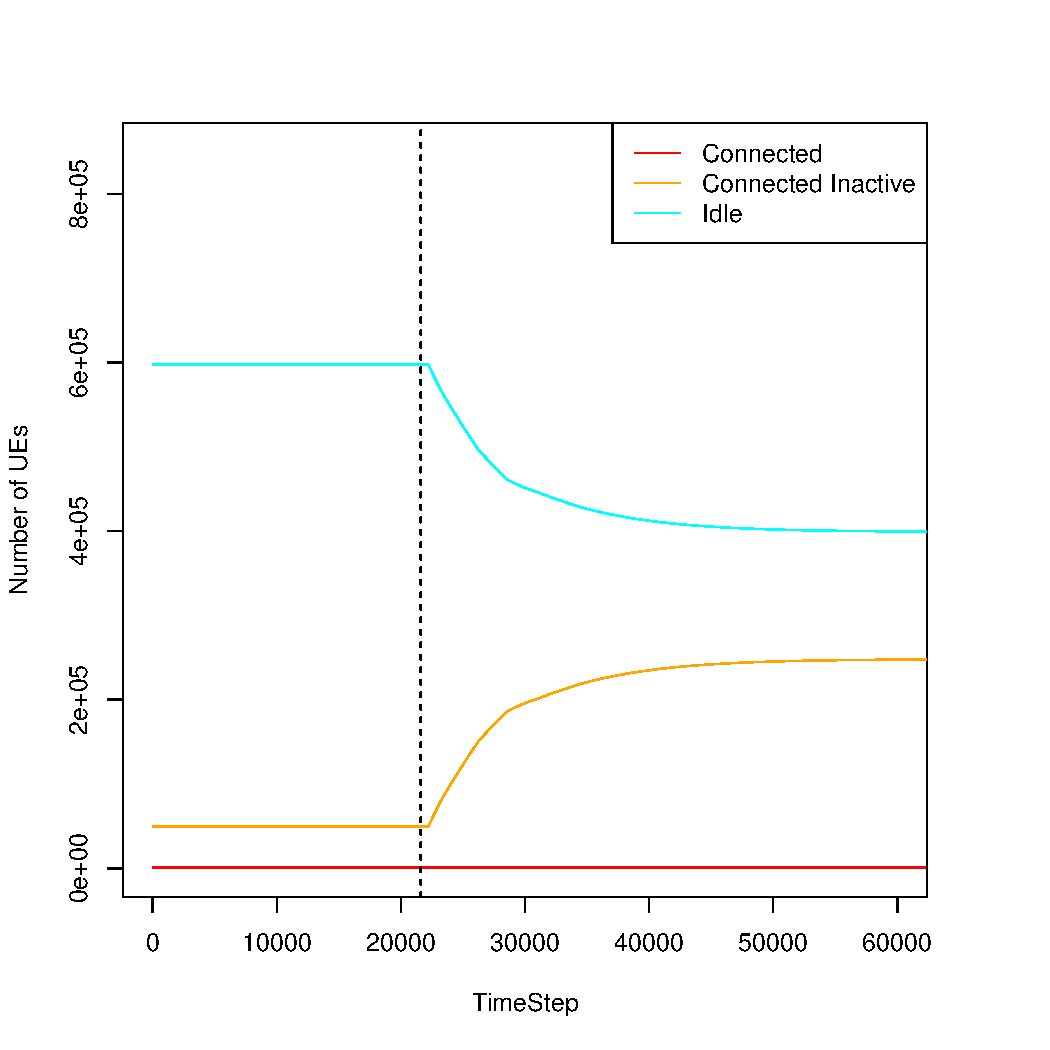
\includegraphics[width=1.0\hsize]{scenario_5_stateBreakdown_86400_345600_1_0_0_0_ideal.pdf}
   \subcaption{各状態にあるUE台数の変化}
   \label{subfig:scenario_5_stateBreakdown_86400_345600_1_0_0_0_ideal}
 \end{subfigure}
 \caption{理想PID($K_p = 1、K_i = 0、K_d = 0$)}
 \label{fig:result_1}
\end{figure}
\begin{figure}[htbp]
 \centering
 \begin{subfigure}{0.49\hsize}
   \centering
   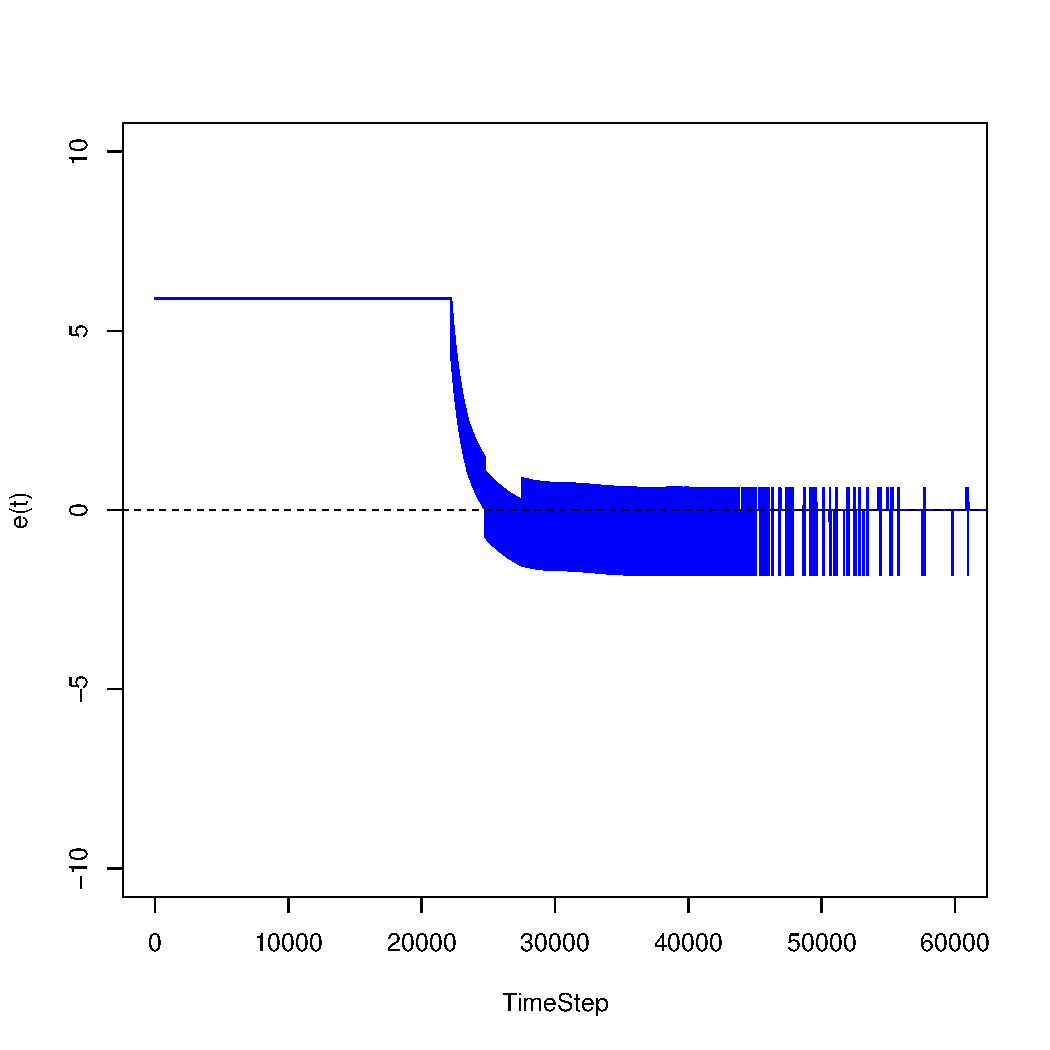
\includegraphics[width=1.0\hsize]{scenario_5_e_86400_345600_2_0_0_0_ideal.pdf}
   \subcaption{$e(t)$の変化}
   \label{subfig:scenario_5_e_86400_345600_0-318_2_0_0_0_ideal}
 \end{subfigure}
 \begin{subfigure}{0.49\hsize}
   \centering
   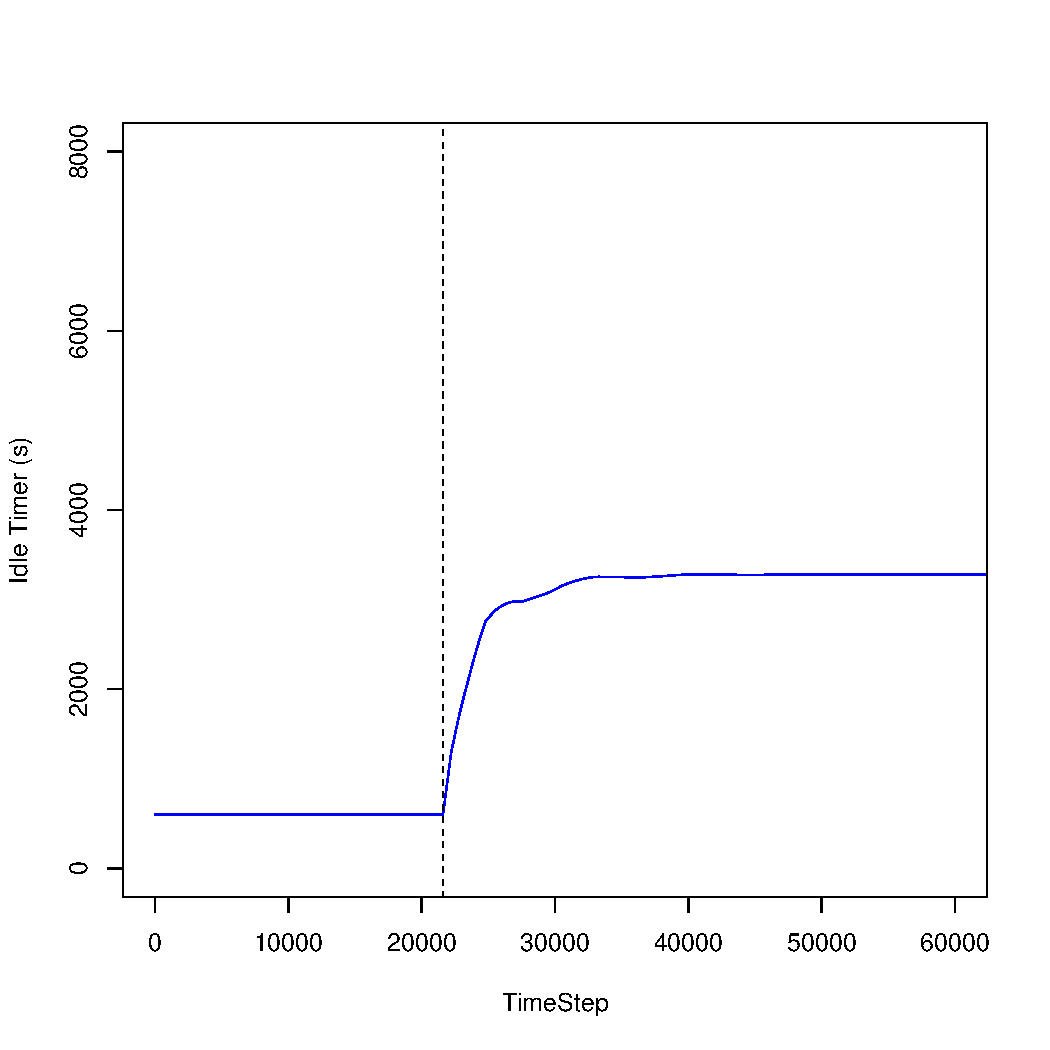
\includegraphics[width=1.0\hsize]{scenario_5_idleTimer_86400_345600_2_0_0_0_ideal.pdf}
   \subcaption{IdleTimerの変化}
   \label{subfig:scenario_5_idleTimer_86400_345600_2_0_0_0_ideal}
 \end{subfigure}
 \par\bigskip %改行
 \begin{subfigure}{0.49\hsize}
   \centering
   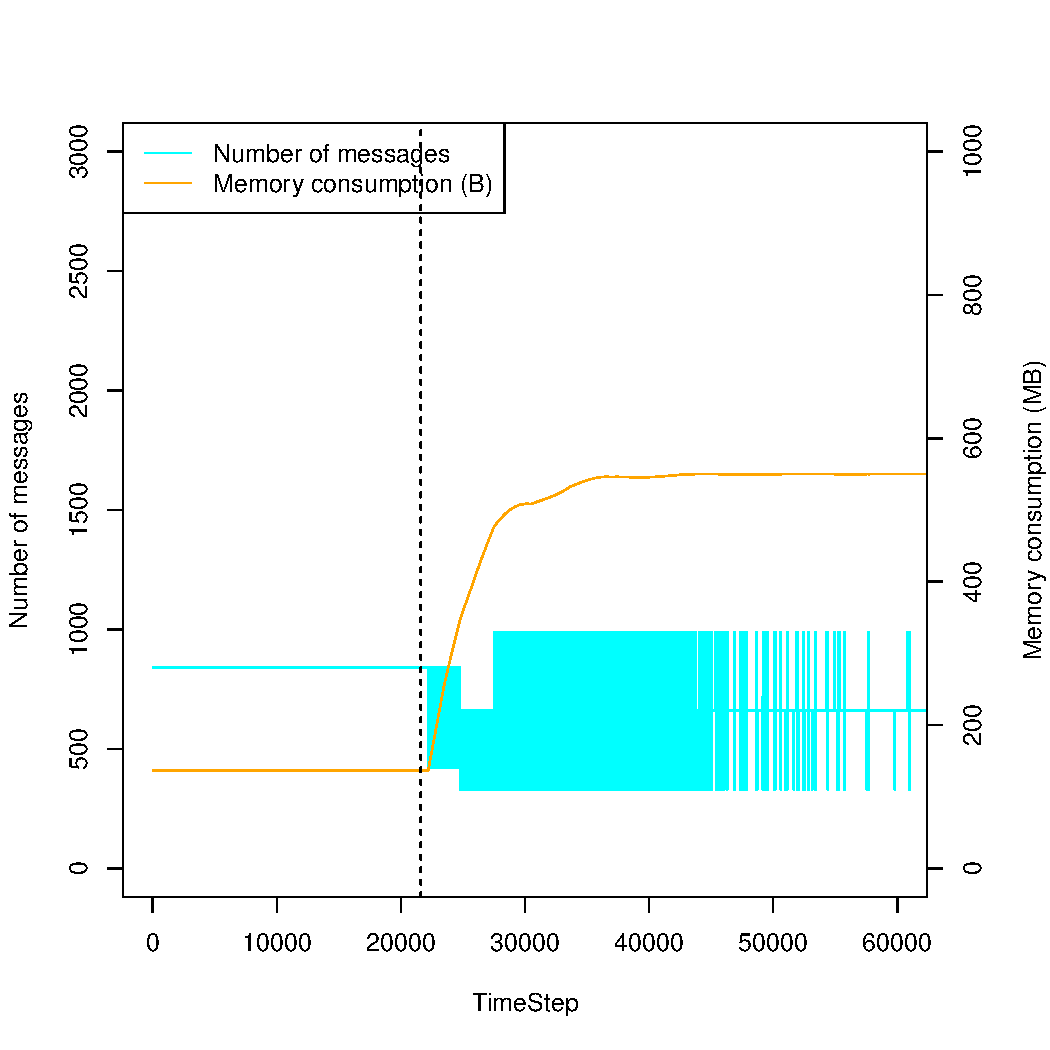
\includegraphics[width=1.0\hsize]{scenario_5_signaling_and_memoryload_vs_timeStep_86400_345600_2_0_0_0_ideal.pdf}
   \subcaption{CPU負荷とメモリ使用量の変化}
   \label{subfig:scenario_5_signaling_and_memoryload_vs_timeStep_86400_345600_2_0_0_0_ideal}
 \end{subfigure}
 \begin{subfigure}{0.49\hsize}
   \centering
   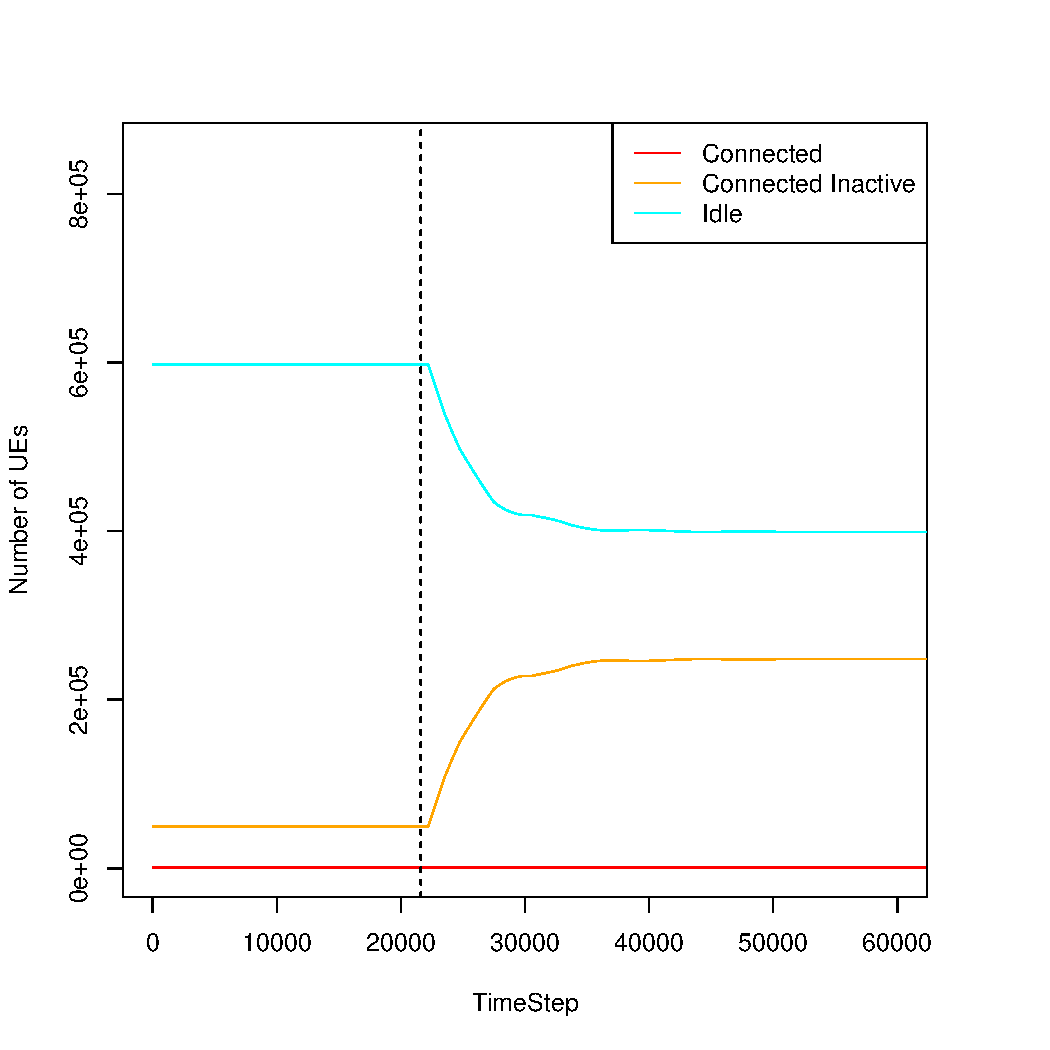
\includegraphics[width=1.0\hsize]{scenario_5_stateBreakdown_86400_345600_2_0_0_0_ideal.pdf}
   \subcaption{各状態にあるUE台数の変化}
   \label{subfig:scenario_5_stateBreakdown_86400_345600_2_0_0_0_ideal}
 \end{subfigure}
 \caption{理想PID($K_p = 2、K_i = 0、K_d = 0$)}
 \label{fig:result_2}
\end{figure}
\begin{figure}[htbp]
 \centering
 \begin{subfigure}{0.49\hsize}
   \centering
   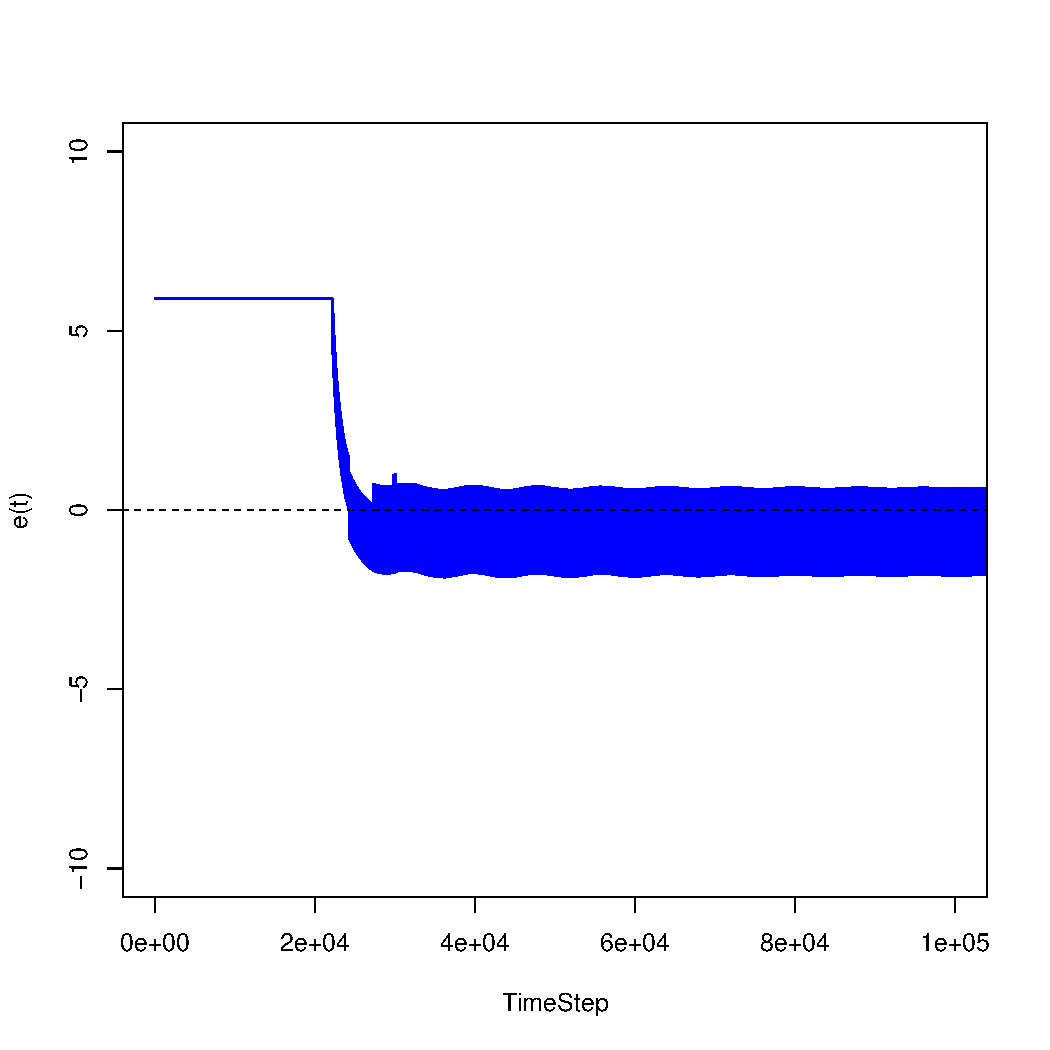
\includegraphics[width=1.0\hsize]{scenario_5_e_long_86400_345600_2-875_0_0_0_ideal.pdf}
   \subcaption{$e(t)$の変化}
   \label{subfig:scenario_5_e_86400_345600_0-318_2-875_0_0_0_ideal}
 \end{subfigure}
 \begin{subfigure}{0.49\hsize}
   \centering
   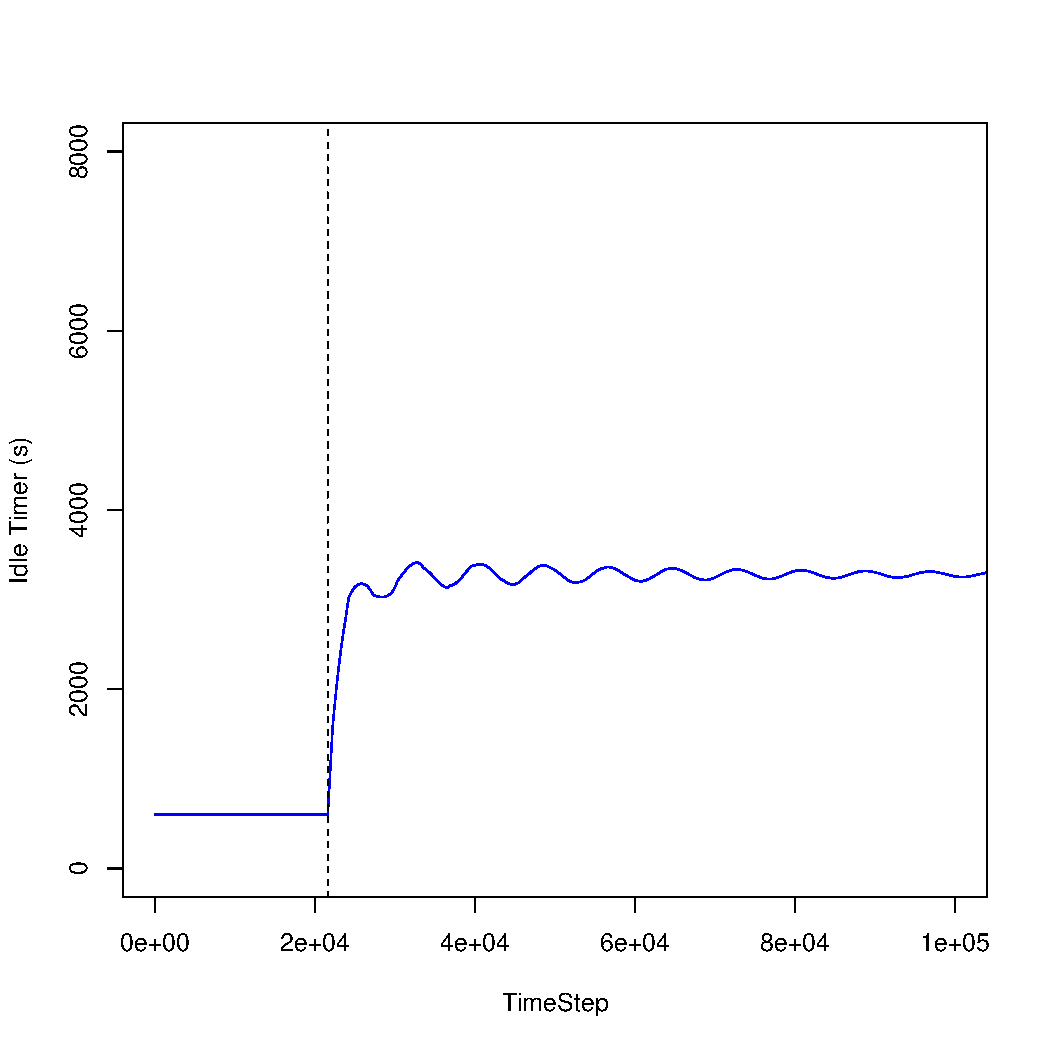
\includegraphics[width=1.0\hsize]{scenario_5_idleTimer_long_86400_345600_2-875_0_0_0_ideal.pdf}
   \subcaption{IdleTimerの変化}
   \label{subfig:scenario_5_idleTimer_86400_345600_2-875_0_0_0_ideal}
 \end{subfigure}
 \par\bigskip %改行
 \begin{subfigure}{0.49\hsize}
   \centering
   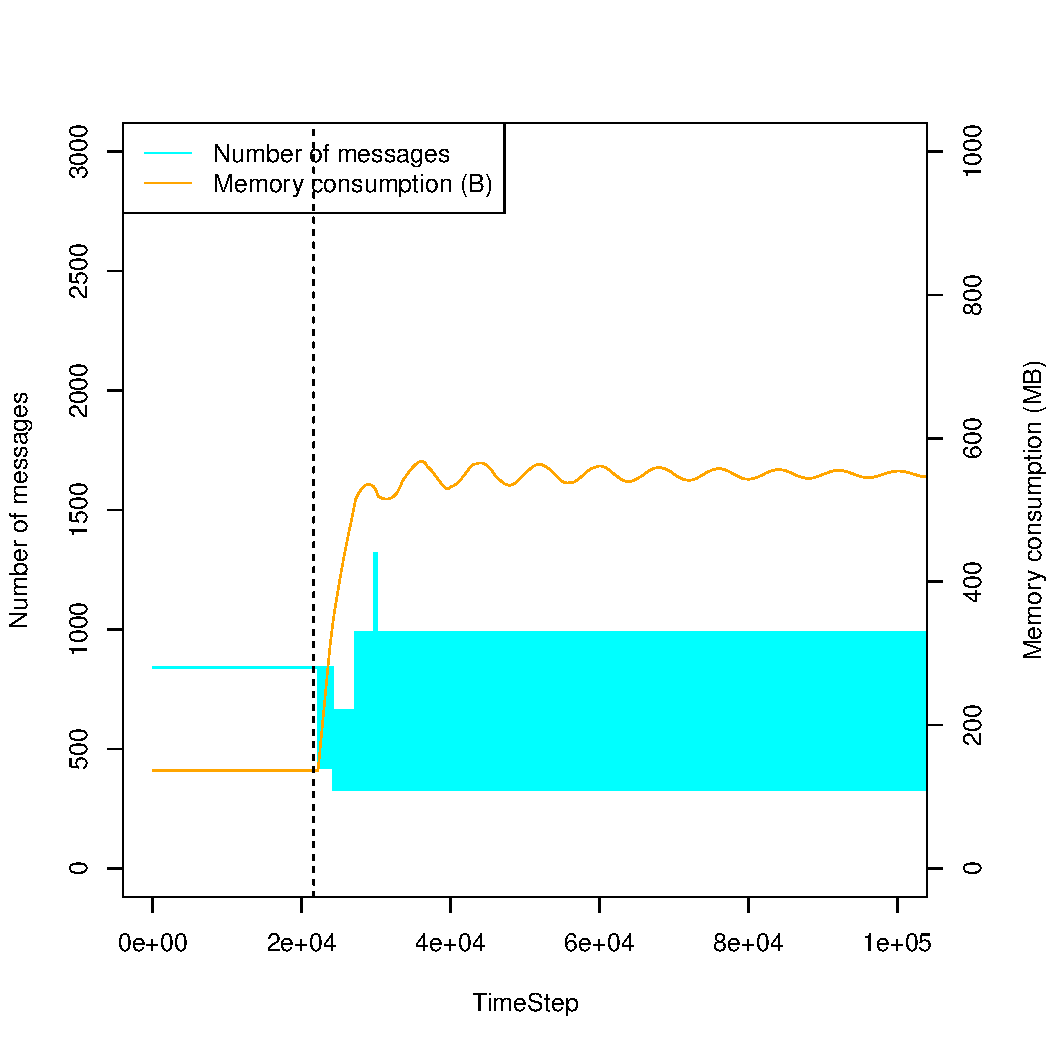
\includegraphics[width=1.0\hsize]{scenario_5_signaling_and_memoryload_vs_timeStep_long_86400_345600_2-875_0_0_0_ideal.pdf}
   \subcaption{CPU負荷とメモリ使用量の変化}
   \label{subfig:scenario_5_signaling_and_memoryload_vs_timeStep_86400_345600_2-875_0_0_0_ideal}
 \end{subfigure}
 \begin{subfigure}{0.49\hsize}
   \centering
   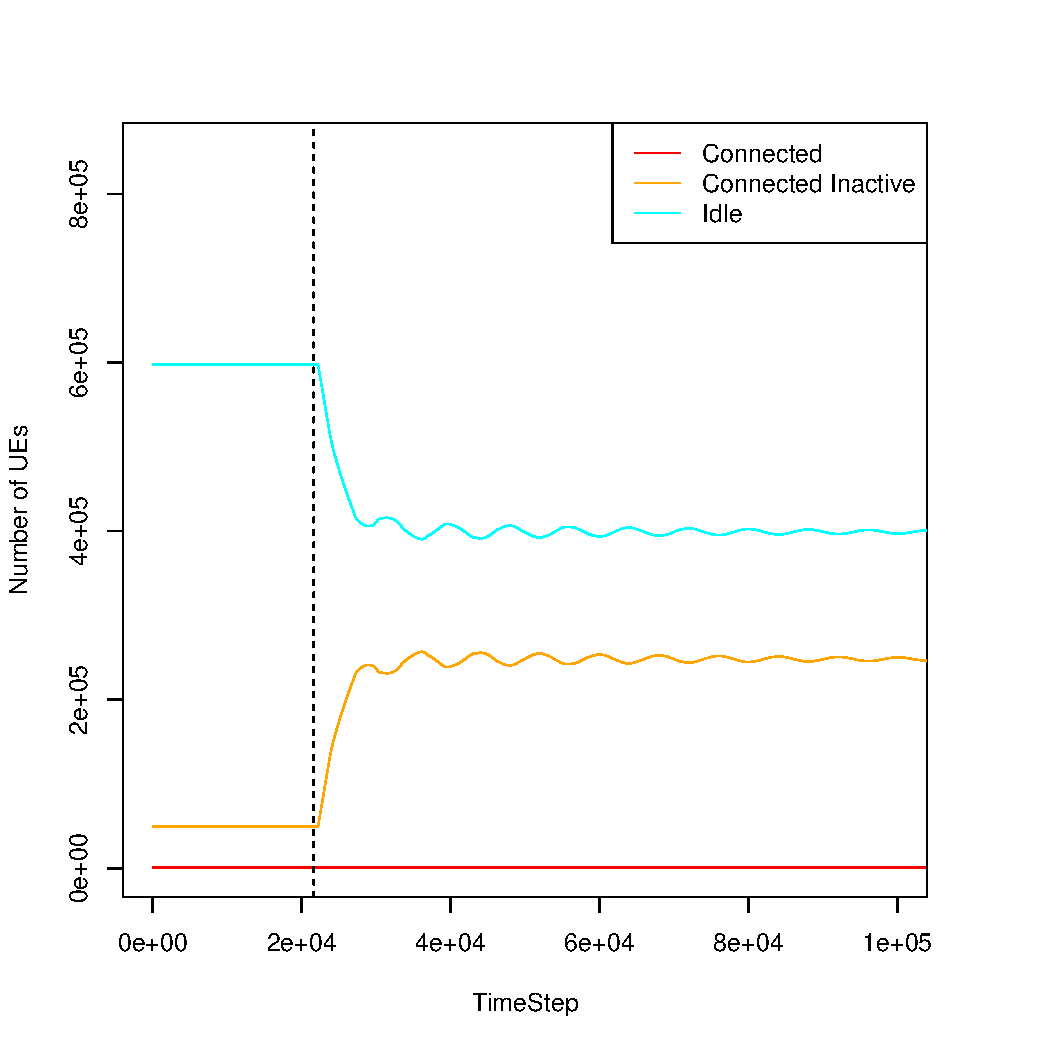
\includegraphics[width=1.0\hsize]{scenario_5_stateBreakdown_long_86400_345600_2-875_0_0_0_ideal.pdf}
   \subcaption{各状態にあるUE台数の変化}
   \label{subfig:scenario_5_stateBreakdown_86400_345600_2-875_0_0_0_ideal}
 \end{subfigure}
 \caption{理想PID($K_p = 2.875、K_i = 0、K_d = 0$)}
 \label{fig:result_3}
\end{figure}
\begin{figure}[htbp]
 \centering
 \begin{subfigure}{0.49\hsize}
   \centering
   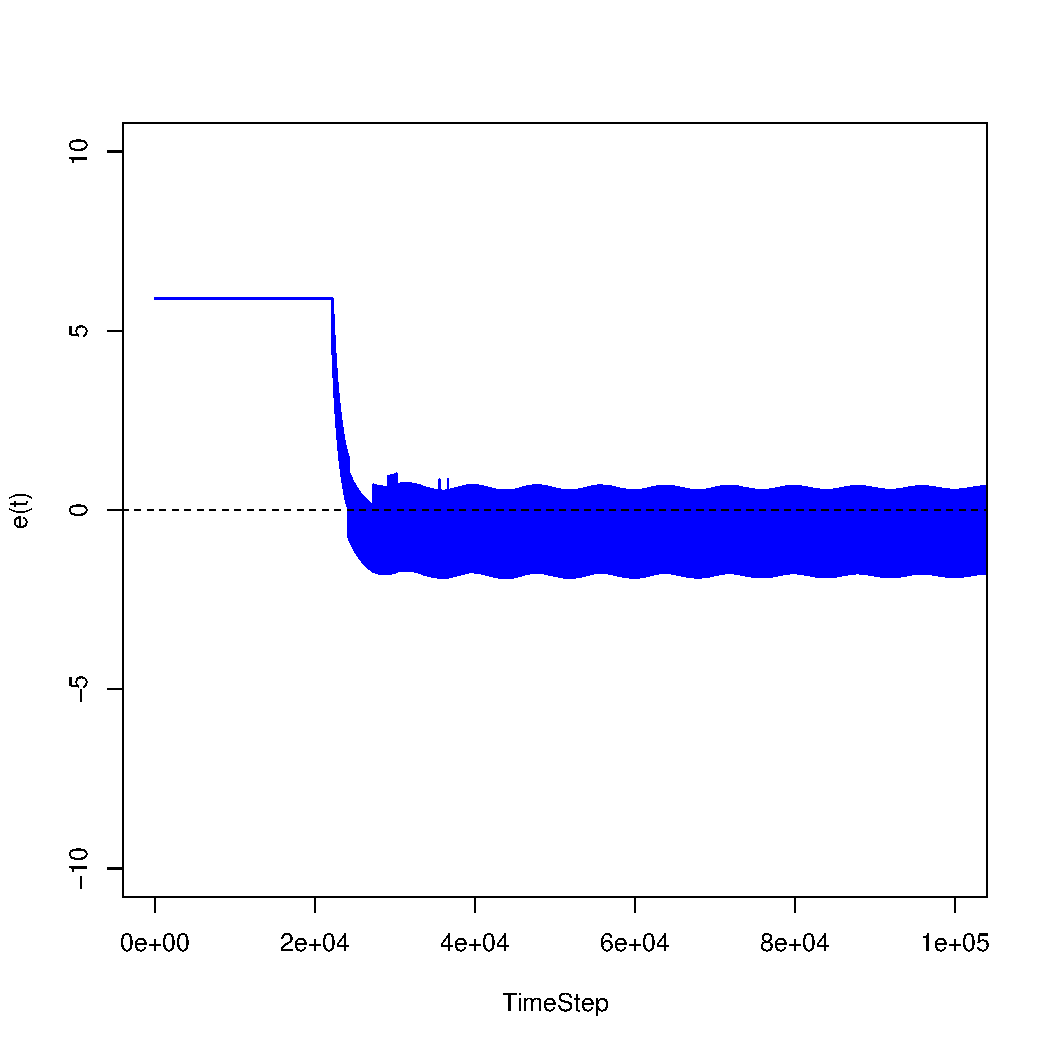
\includegraphics[width=1.0\hsize]{scenario_5_e_long_86400_345600_3_0_0_0_ideal.pdf}
   \subcaption{$e(t)$の変化}
   \label{subfig:scenario_5_e_86400_345600_0-318_3_0_0_0_ideal}
 \end{subfigure}
 \begin{subfigure}{0.49\hsize}
   \centering
   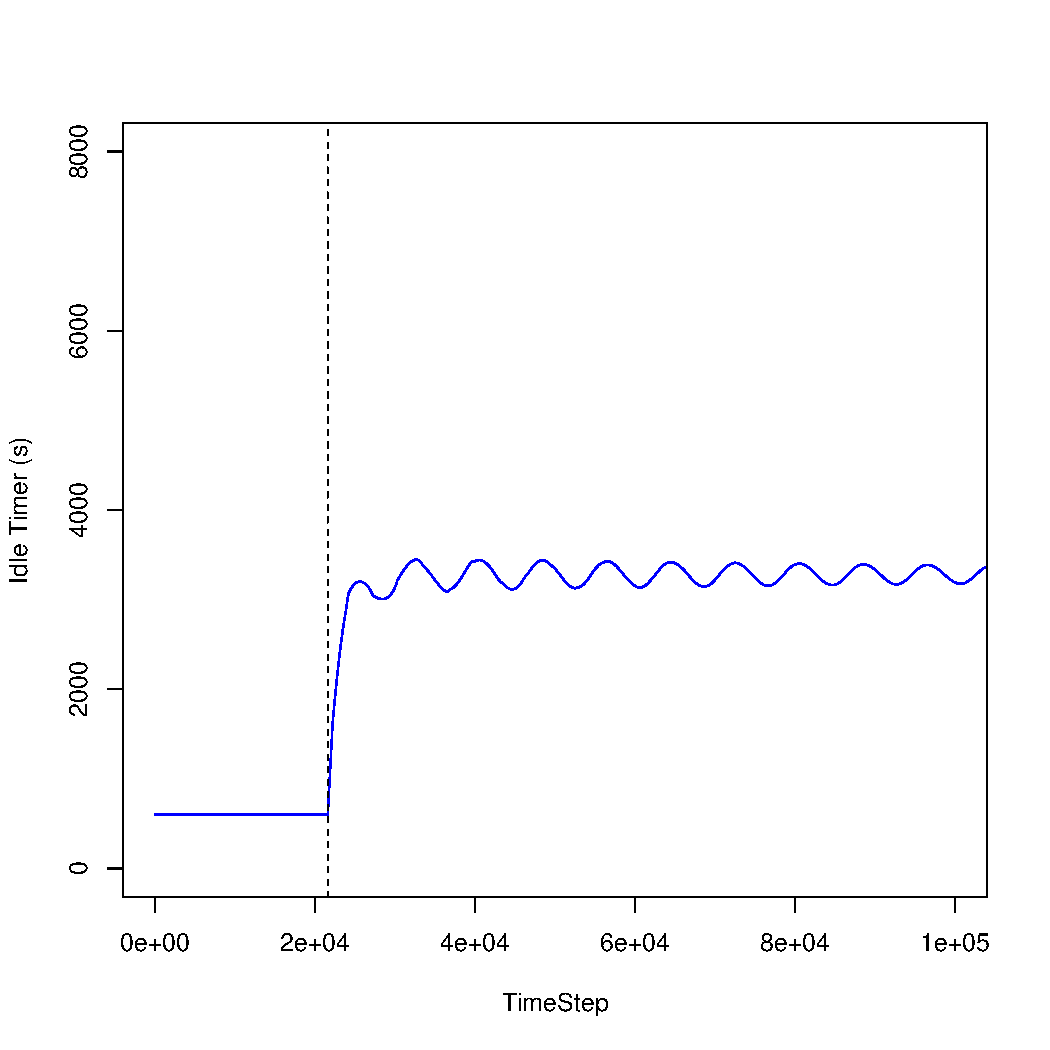
\includegraphics[width=1.0\hsize]{scenario_5_idleTimer_long_86400_345600_3_0_0_0_ideal.pdf}
   \subcaption{IdleTimerの変化}
   \label{subfig:scenario_5_idleTimer_86400_345600_3_0_0_0_ideal}
 \end{subfigure}
 \par\bigskip %改行
 \begin{subfigure}{0.49\hsize}
   \centering
   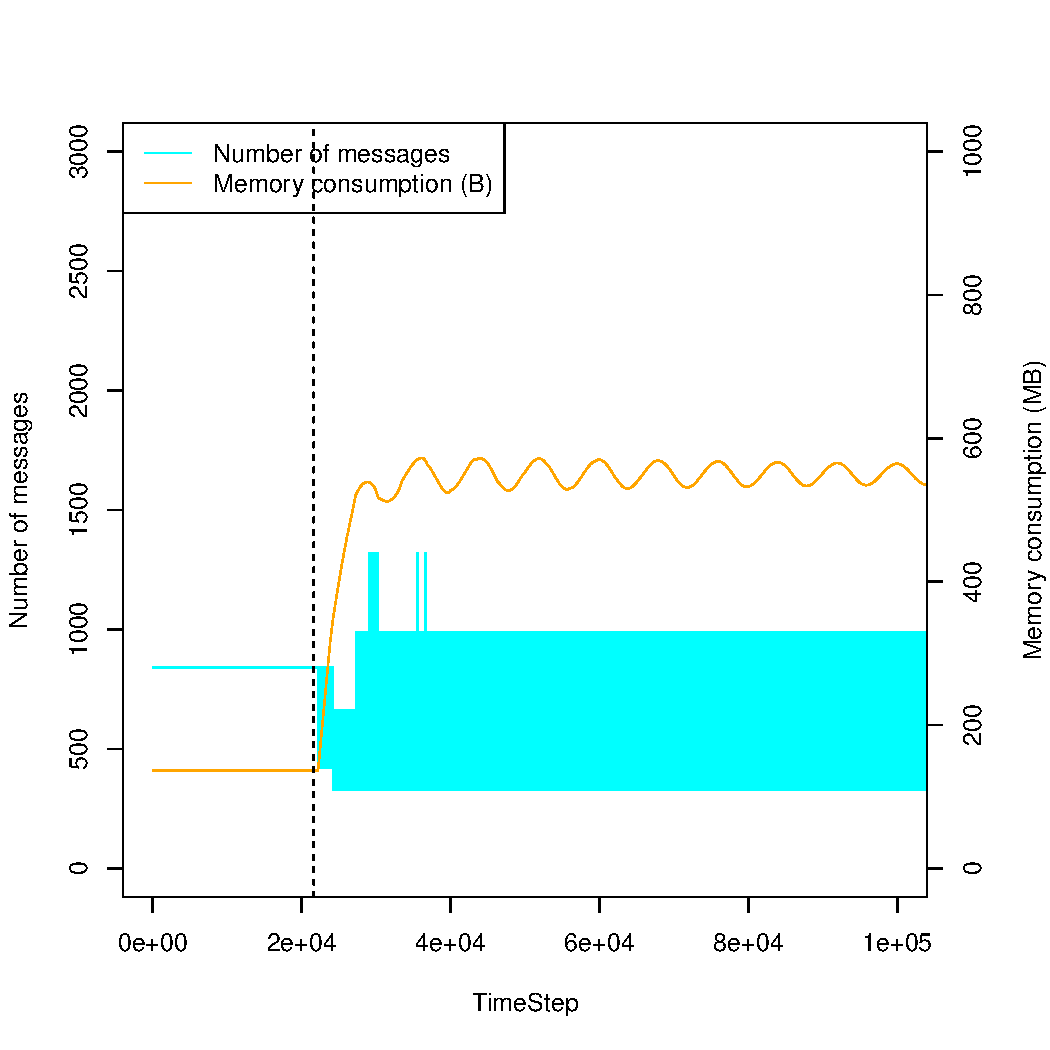
\includegraphics[width=1.0\hsize]{scenario_5_signaling_and_memoryload_vs_timeStep_long_86400_345600_3_0_0_0_ideal.pdf}
   \subcaption{CPU負荷とメモリ使用量の変化}
   \label{subfig:scenario_5_signaling_and_memoryload_vs_timeStep_86400_345600_3_0_0_0_ideal}
 \end{subfigure}
 \begin{subfigure}{0.49\hsize}
   \centering
   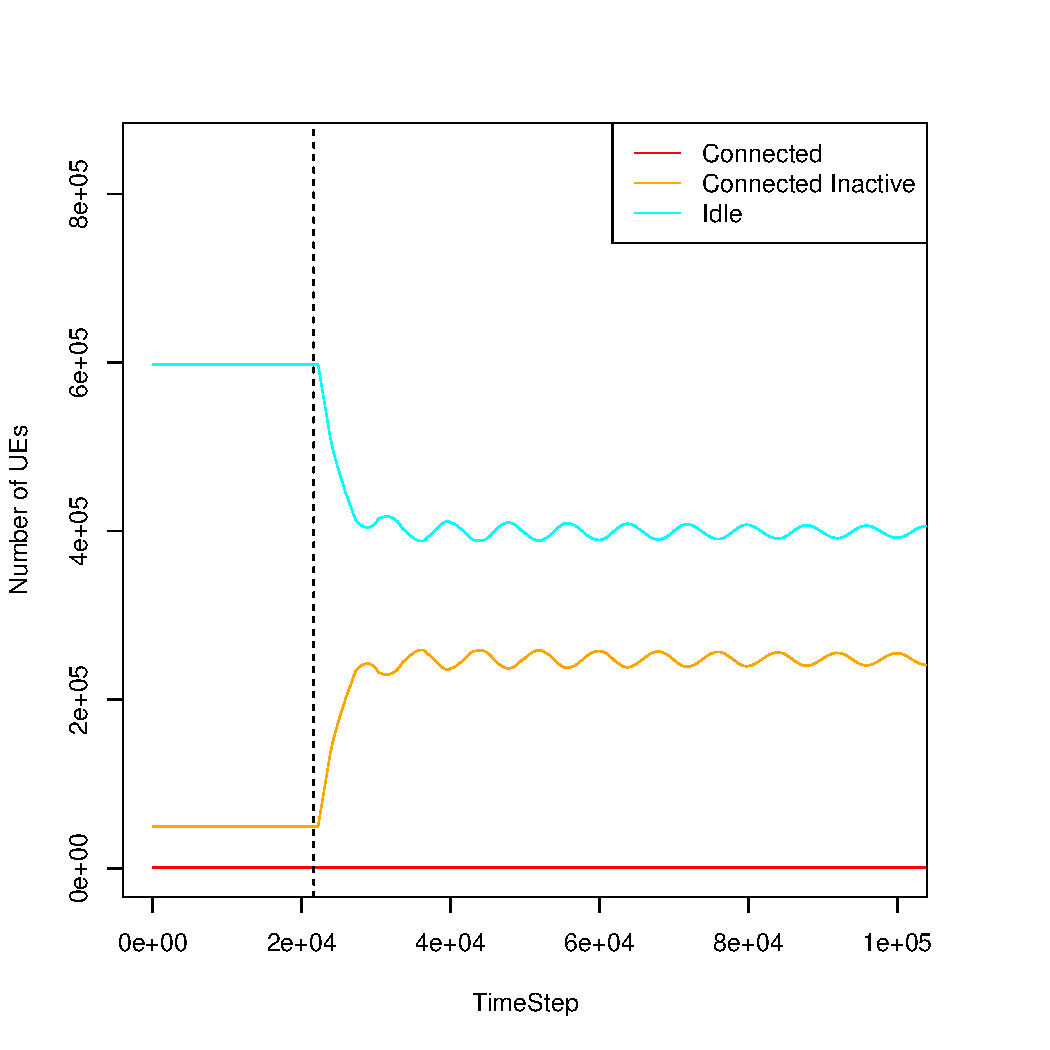
\includegraphics[width=1.0\hsize]{scenario_5_stateBreakdown_long_86400_345600_3_0_0_0_ideal.pdf}
   \subcaption{各状態にあるUE台数の変化}
   \label{subfig:scenario_5_stateBreakdown_86400_345600_3_0_0_0_ideal}
 \end{subfigure}
 \caption{理想PID($K_p = 3、K_i = 0、K_d = 0$)}
 \label{fig:result_4}
\end{figure}

\clearpage
以上の結果より、各ゲインの値は表\ref{table:Ziegler-Nichols_setting}のように求まる。
\begin{table}[]
  \centering
  \caption{ジーグラ・ニコルスの限界感度法に基づく設定}
  \label{table:Ziegler-Nichols_setting}
  \begin{tabular}{c|c|c|c|c|c}
    \hline
    制御の種類  & $K_p$ & $K_i$ & $K_d$ &$T_i$&$T_d$  \\\hline \hline
    P & 1.5 & 0 & 0 & - & - \\
    PI & 1.35 & 0.000203 & 0 & 6640 & -\\
    PID & 1.8 & 0.00045 & 1800 & 4000 & 1000 \\\hline
  \end{tabular}
\end{table}
% \begin{table}[]
%   \centering
%   \caption{ジーグラ・ニコルスの限界感度法に基づく設定}
%   \label{table:Ziegler-Nichols_setting}
%   \begin{tabular}{c|c|c|c}
%     \hline
%     制御の種類  & $K_p$ & $T_i$ & $T_d$ \\\hline \hline
%     P & 0.265 & - & - \\
%     PI & 0.2385 & 6183.5 & - \\
%     PID & 0.318 & 3725 & 931.25 \\\hline
%   \end{tabular}
% \end{table}


\clearpage
表\ref{table:Ziegler-Nichols_setting}に示したP制御の値を$K_p$、$K_i$および$K_d$にそれぞれ設定した場合の評価結果を図\ref{fig:result_p}に示す。
\begin{figure}[htbp]
 \centering
 \begin{subfigure}{0.49\hsize}
   \centering
   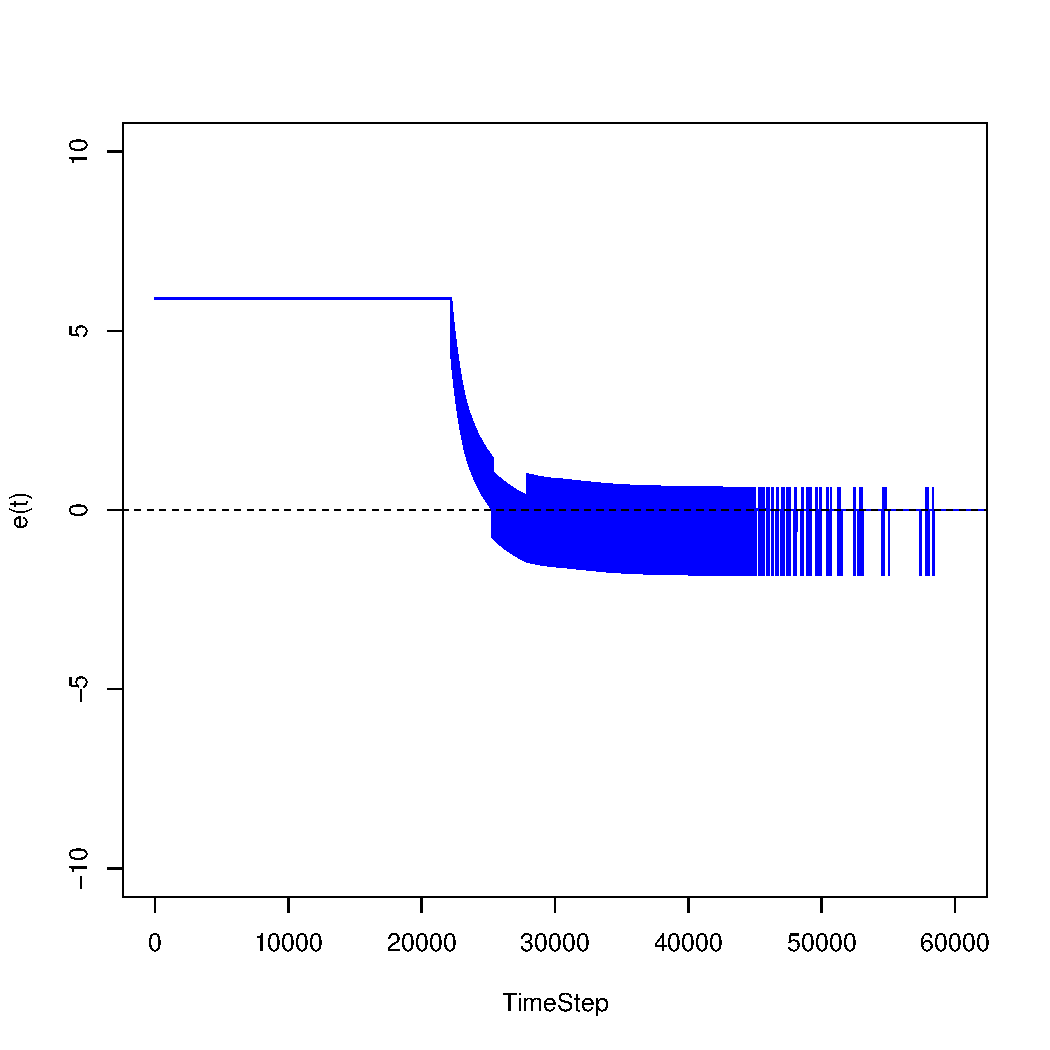
\includegraphics[width=1.0\hsize]{scenario_5_e_86400_345600_1-5_0_0_0_ideal.pdf}
   \subcaption{$e(t)$の変化}
   \label{subfig:scenario_5_e_86400_345600_0-318_1-5_0_0_0_ideal}
 \end{subfigure}
 \begin{subfigure}{0.49\hsize}
   \centering
   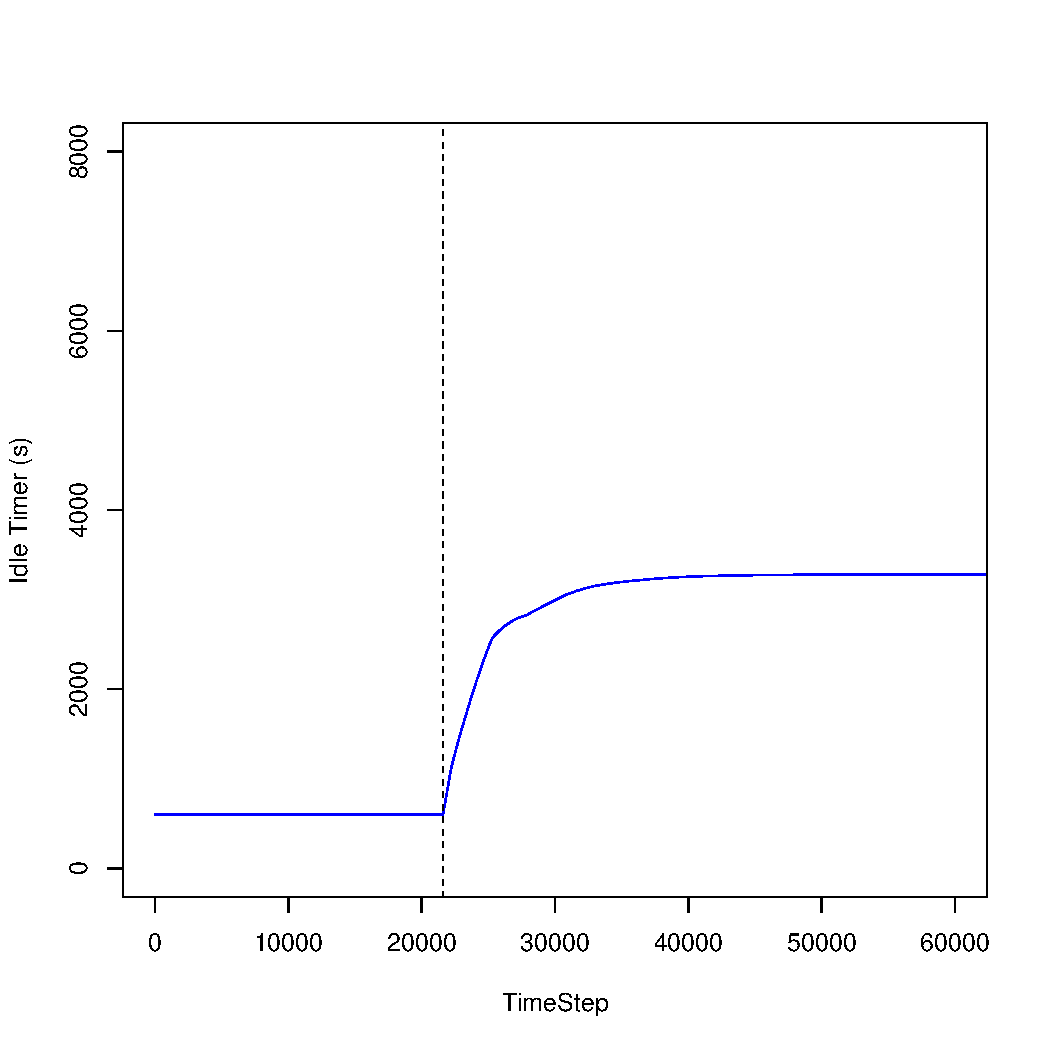
\includegraphics[width=1.0\hsize]{scenario_5_idleTimer_86400_345600_1-5_0_0_0_ideal.pdf}
   \subcaption{IdleTimerの変化}
   \label{subfig:scenario_5_idleTimer_86400_345600_1-5_0_0_0_ideal}
 \end{subfigure}
 \par\bigskip %改行
 \begin{subfigure}{0.49\hsize}
   \centering
   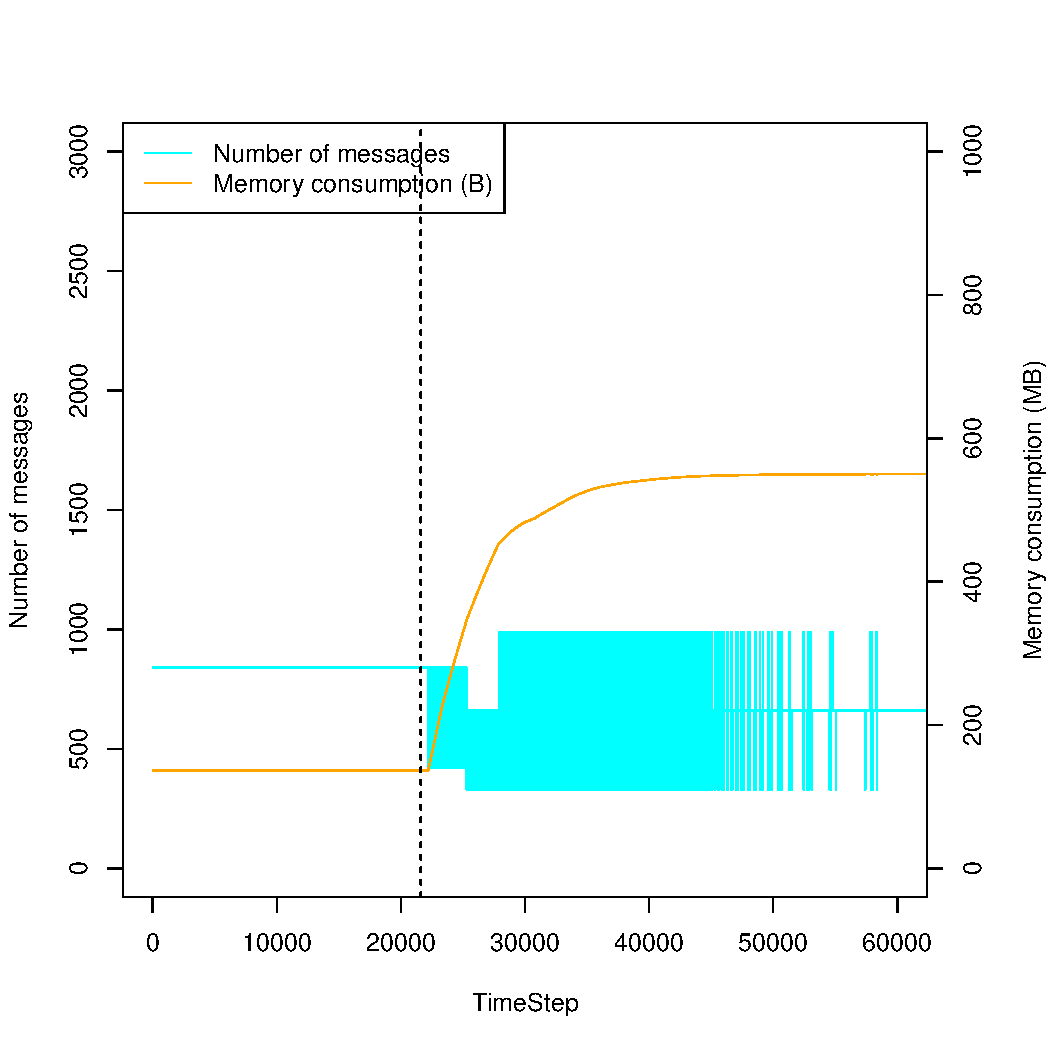
\includegraphics[width=1.0\hsize]{scenario_5_signaling_and_memoryload_vs_timeStep_86400_345600_1-5_0_0_0_ideal.pdf}
   \subcaption{CPU負荷とメモリ使用量の変化}
   \label{subfig:scenario_5_signaling_and_memoryload_vs_timeStep_86400_345600_1-5_0_0_0_ideal}
 \end{subfigure}
 \begin{subfigure}{0.49\hsize}
   \centering
   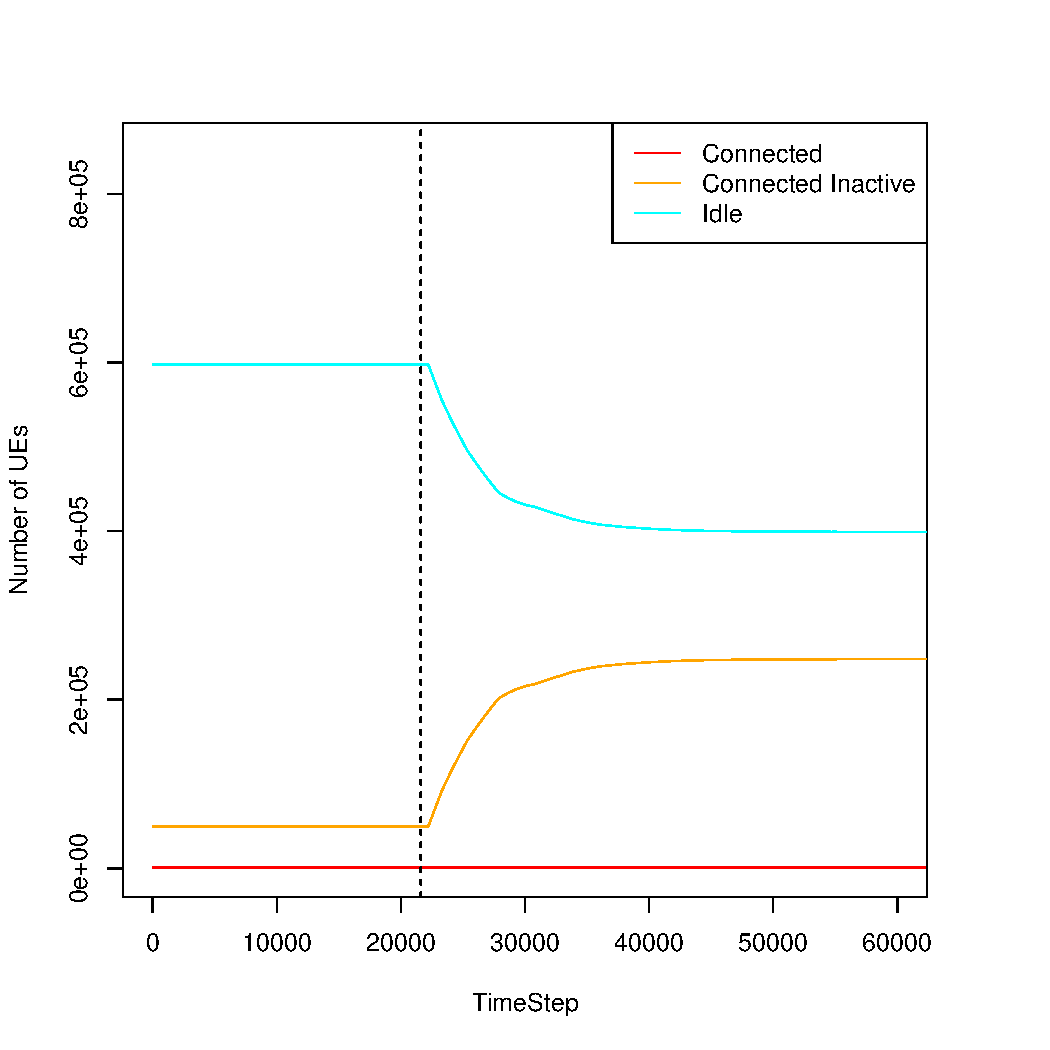
\includegraphics[width=1.0\hsize]{scenario_5_stateBreakdown_86400_345600_1-5_0_0_0_ideal.pdf}
   \subcaption{各状態にあるUE台数の変化}
   \label{subfig:scenario_5_stateBreakdown_86400_345600_1-5_0_0_0_ideal}
 \end{subfigure}
 \caption{理想PID($K_p = 1.5、K_i = 0、K_d = 0$)}
 \label{fig:result_p}
\end{figure}
\clearpage
表\ref{table:Ziegler-Nichols_setting}に示したPI制御の値を$K_p$、$K_i$および$K_d$にそれぞれ設定した場合の評価結果を図\ref{fig:result_pi}に示す。
\begin{figure}[htbp]
 \centering
 \begin{subfigure}{0.49\hsize}
   \centering
   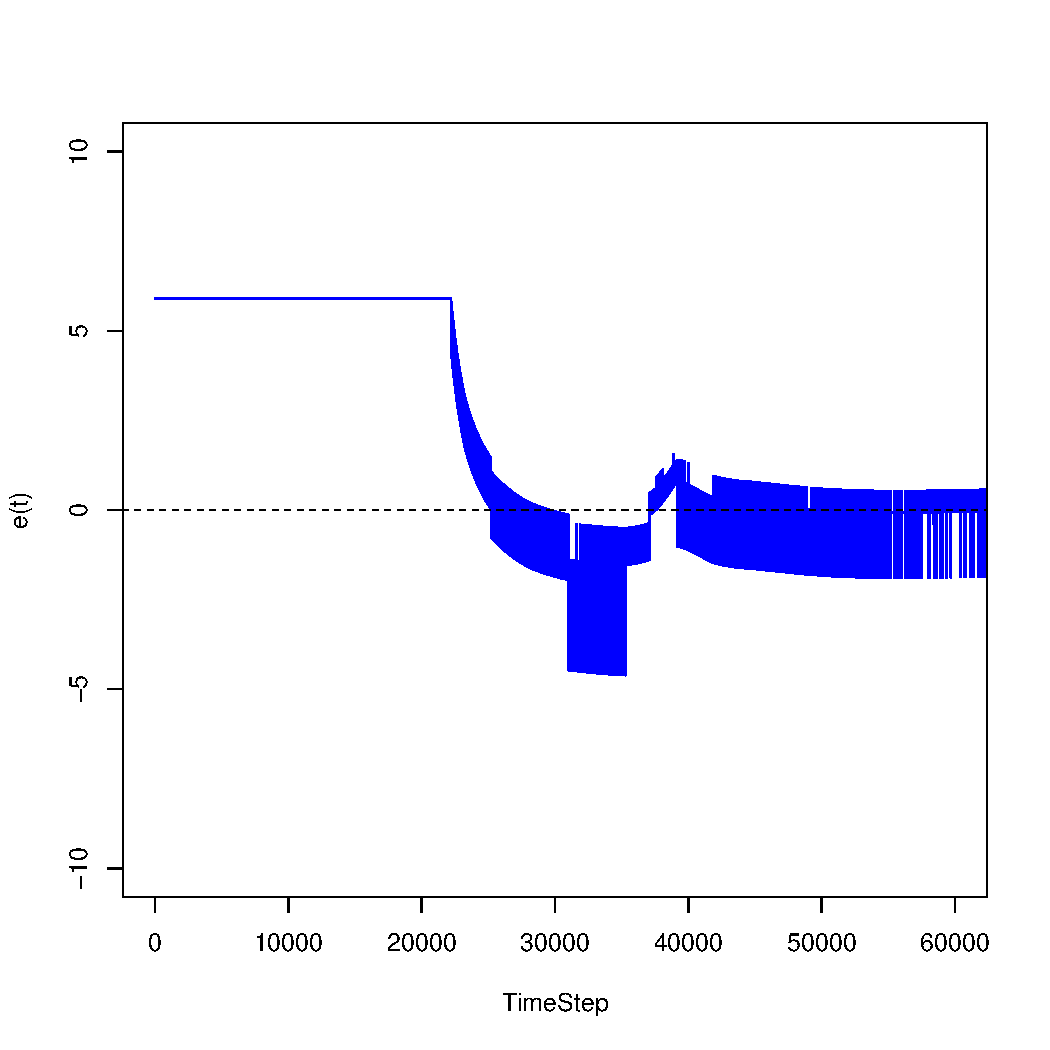
\includegraphics[width=1.0\hsize]{scenario_5_e_86400_345600_1-35_0-000203_0_0_ideal.pdf}
   \subcaption{$e(t)$の変化}
   \label{subfig:scenario_5_e_86400_345600_0-318_1-35_0-000203_0_0_ideal}
 \end{subfigure}
 \begin{subfigure}{0.49\hsize}
   \centering
   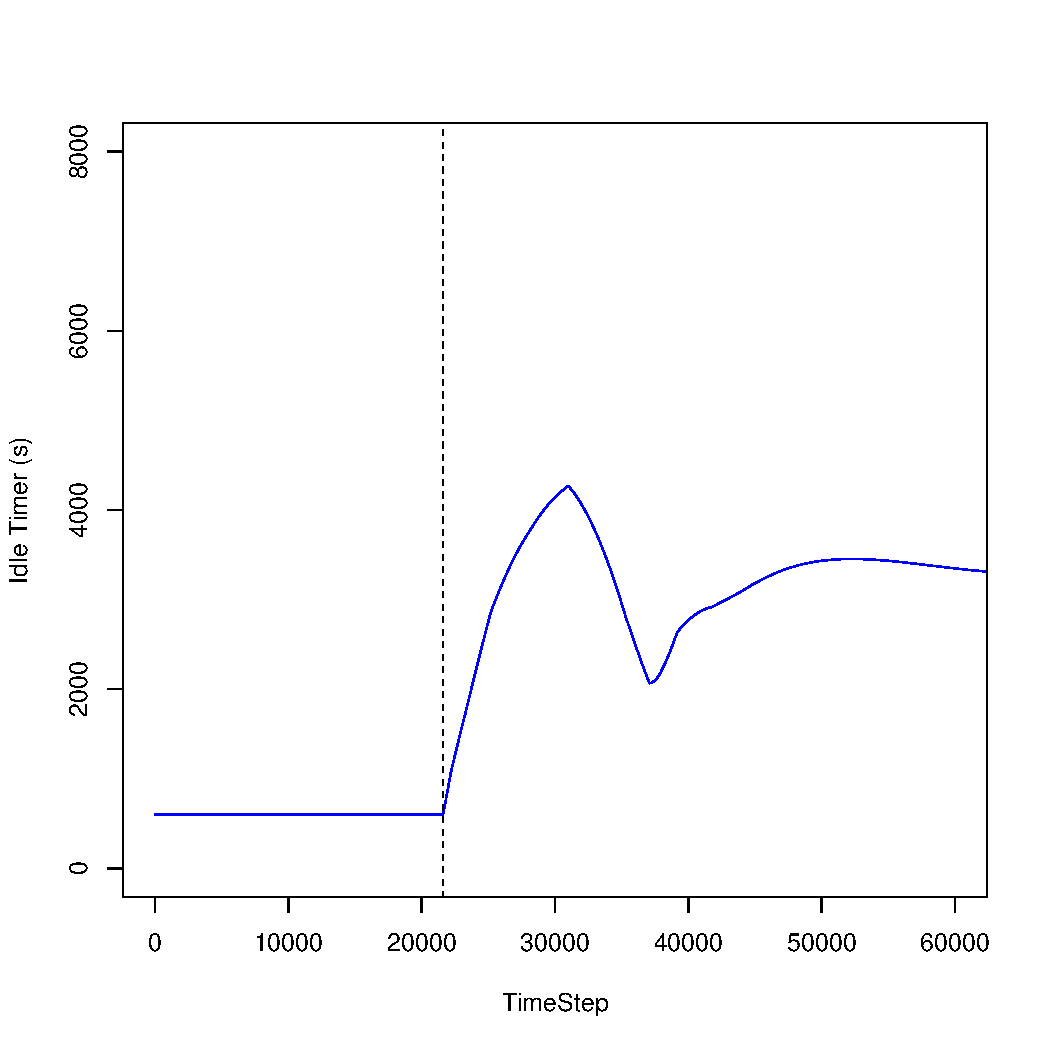
\includegraphics[width=1.0\hsize]{scenario_5_idleTimer_86400_345600_1-35_0-000203_0_0_ideal.pdf}
   \subcaption{IdleTimerの変化}
   \label{subfig:scenario_5_idleTimer_86400_345600_1-35_0-000203_0_0_ideal}
 \end{subfigure}
 \par\bigskip %改行
 \begin{subfigure}{0.49\hsize}
   \centering
   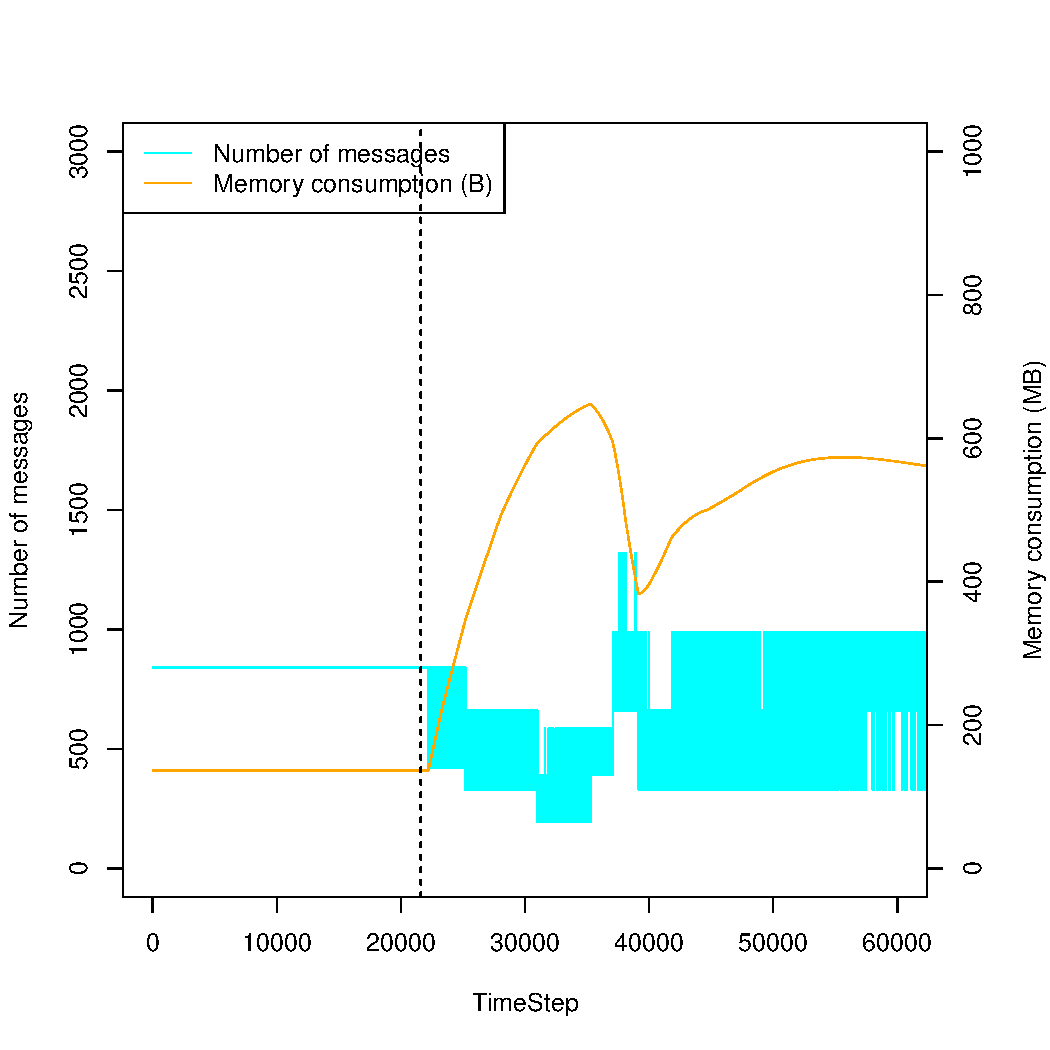
\includegraphics[width=1.0\hsize]{scenario_5_signaling_and_memoryload_vs_timeStep_86400_345600_1-35_0-000203_0_0_ideal.pdf}
   \subcaption{CPU負荷とメモリ使用量の変化}
   \label{subfig:scenario_5_signaling_and_memoryload_vs_timeStep_86400_345600_1-35_0-000203_0_0_ideal}
 \end{subfigure}
 \begin{subfigure}{0.49\hsize}
   \centering
   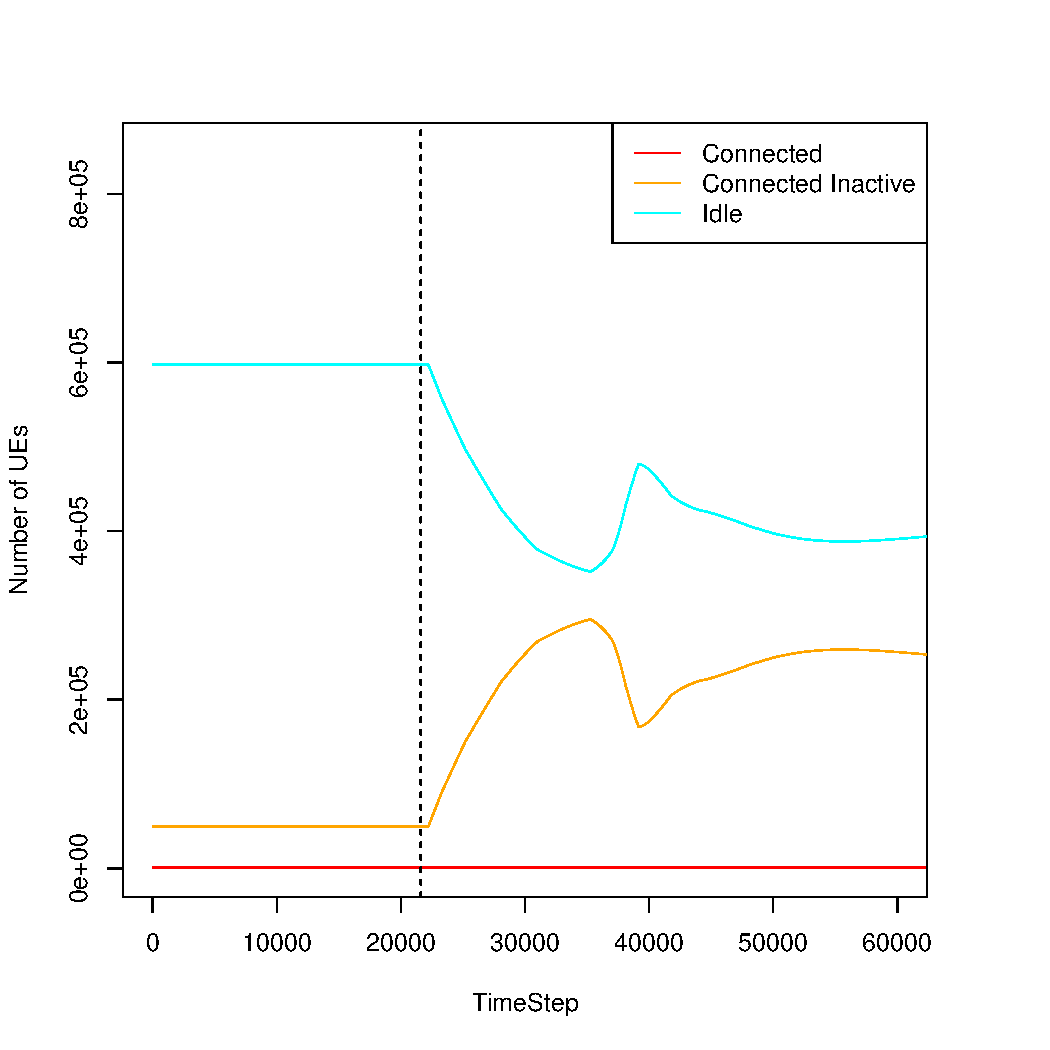
\includegraphics[width=1.0\hsize]{scenario_5_stateBreakdown_86400_345600_1-35_0-000203_0_0_ideal.pdf}
   \subcaption{各状態にあるUE台数の変化}
   \label{subfig:scenario_5_stateBreakdown_86400_345600_1-35_0-000203_0_0_ideal}
 \end{subfigure}
 \caption{理想PID($K_p = 1.35、K_i = 0.000203、K_d = 0$)}
 \label{fig:result_pi}
\end{figure}
\clearpage
表\ref{table:Ziegler-Nichols_setting}に示したPID制御の値を$K_p$、$K_i$および$K_d$にそれぞれ設定した場合の評価結果を図\ref{fig:result_pid}に示す。
\begin{figure}[htbp]
 \centering
 \begin{subfigure}{0.49\hsize}
   \centering
   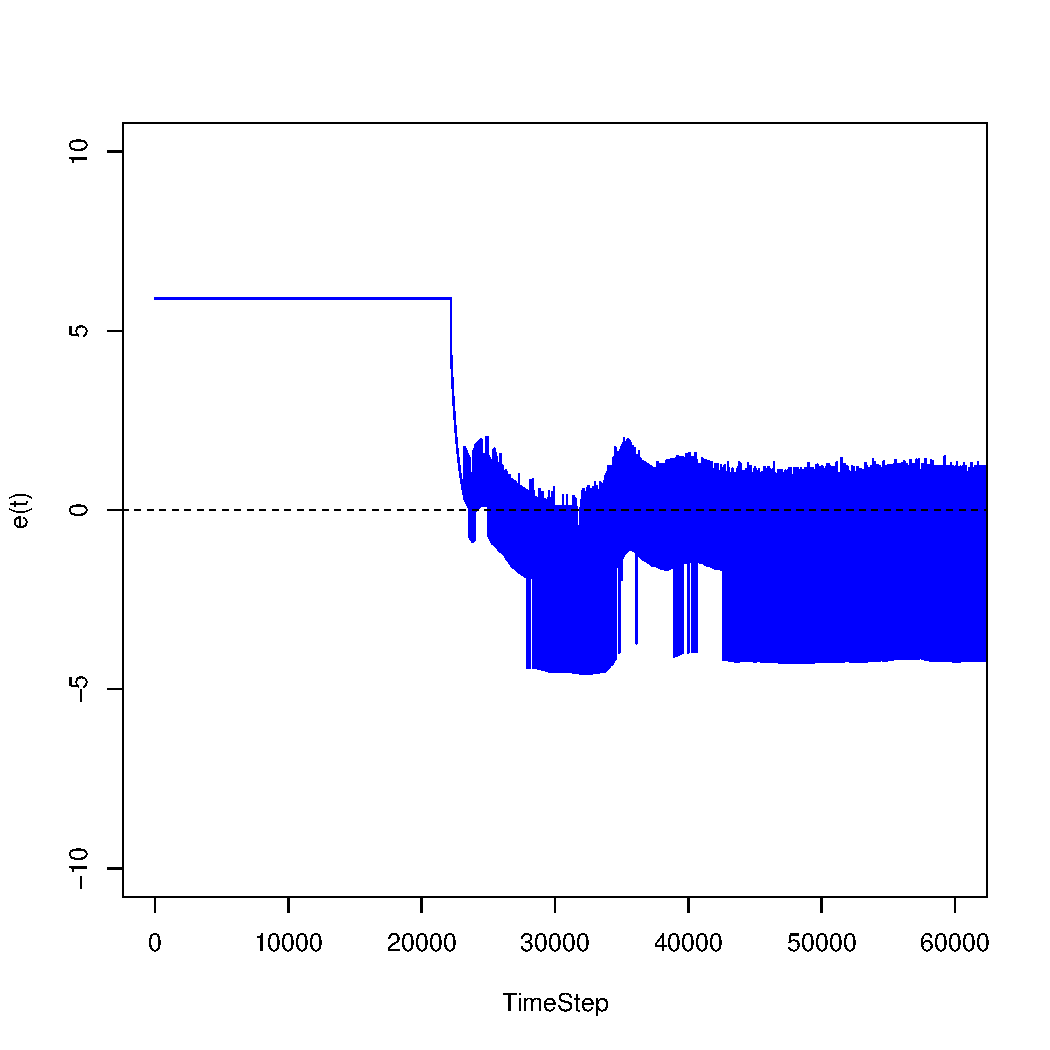
\includegraphics[width=1.0\hsize]{scenario_5_e_86400_345600_1-8_0-00045_1800_0_ideal.pdf}
   \subcaption{$e(t)$の変化}
   \label{subfig:scenario_5_e_86400_345600_0-318_1-8_0-00045_1800_0_ideal}
 \end{subfigure}
 \begin{subfigure}{0.49\hsize}
   \centering
   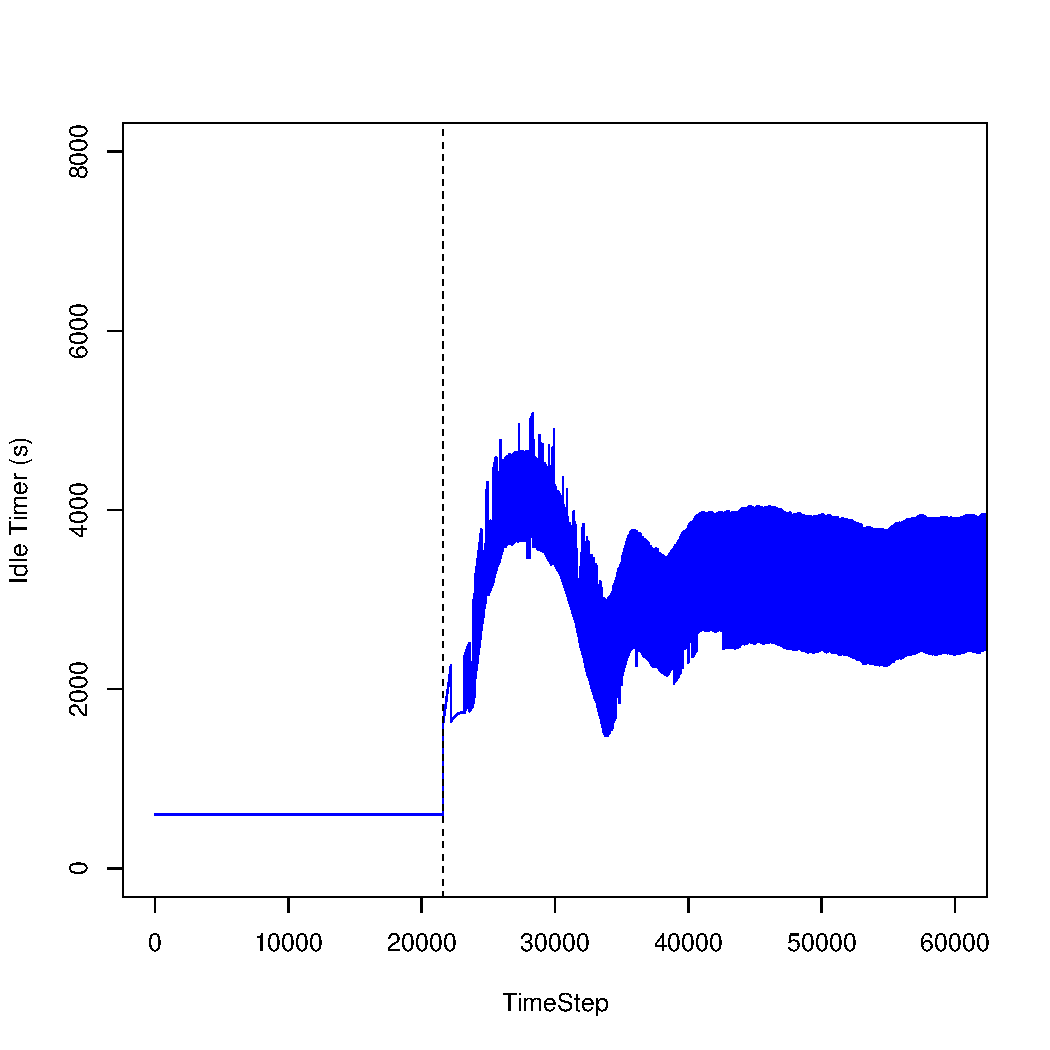
\includegraphics[width=1.0\hsize]{scenario_5_idleTimer_86400_345600_1-8_0-00045_1800_0_ideal.pdf}
   \subcaption{IdleTimerの変化}
   \label{subfig:scenario_5_idleTimer_86400_345600_1-8_0-00045_1800_0_ideal}
 \end{subfigure}
 \par\bigskip %改行
 \begin{subfigure}{0.49\hsize}
   \centering
   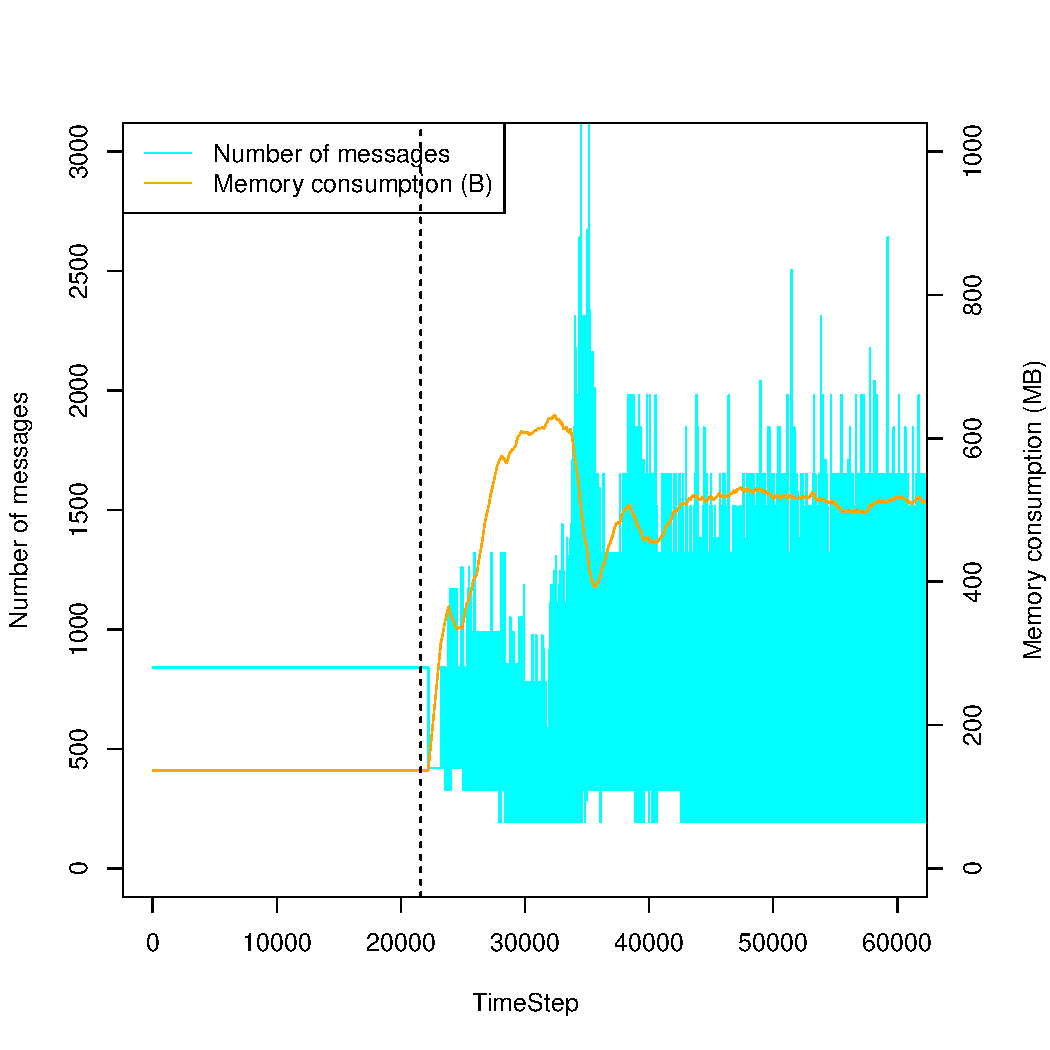
\includegraphics[width=1.0\hsize]{scenario_5_signaling_and_memoryload_vs_timeStep_86400_345600_1-8_0-00045_1800_0_ideal.pdf}
   \subcaption{CPU負荷とメモリ使用量の変化}
   \label{subfig:scenario_5_signaling_and_memoryload_vs_timeStep_86400_345600_1-8_0-00045_1800_0_ideal}
 \end{subfigure}
 \begin{subfigure}{0.49\hsize}
   \centering
   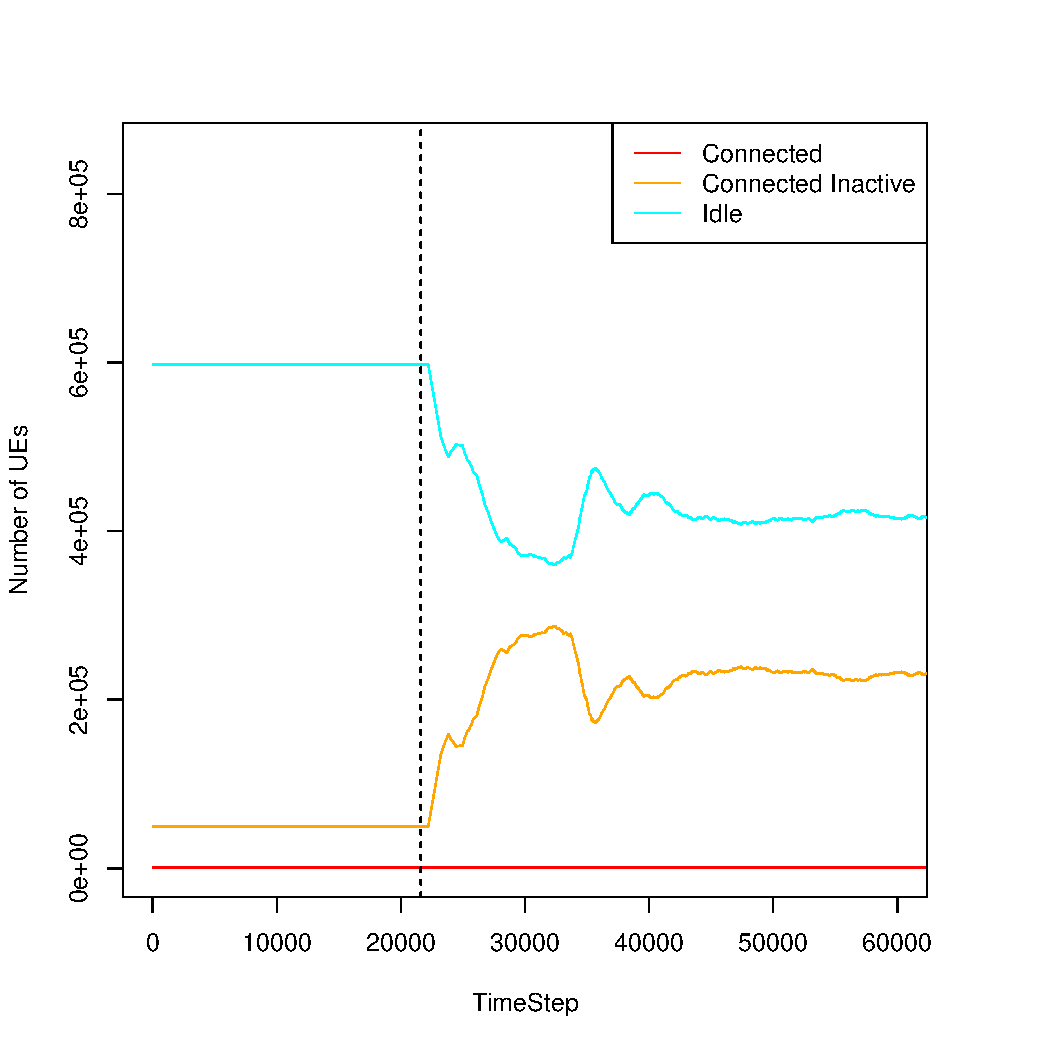
\includegraphics[width=1.0\hsize]{scenario_5_stateBreakdown_86400_345600_1-8_0-00045_1800_0_ideal.pdf}
   \subcaption{各状態にあるUE台数の変化}
   \label{subfig:scenario_5_stateBreakdown_86400_345600_1-8_0-00045_1800_0_ideal}
 \end{subfigure}
 \caption{理想PID($K_p = 1.8、K_i = 0.00045、K_d = 1800$)}
 \label{fig:result_pid}
\end{figure}



\clearpage
以上の図\ref{fig:result_p}、\ref{fig:result_pi}図\ref{fig:result_pid}を比較すると、図\ref{fig:result_p}に示したP制御が最も制御が安定していることがわかる。また、$E(t)$が0に収束するまでの時間も最も短くなっている。以上の結果より、比例ゲインに 1.5 を設定したP制御がIdleタイマの制御に最も適していると言える。

一方で、PI制御は、P制御と比較して良い結果が得られなかった。積分ゲインを利用しても制御が改善しなかった理由は、比例ゲインのみで制御した場合に発生するオフセット(定常偏差)が小さいことがあげられる。オフセットとは、定常状態の時に出力値と目標値の差である。一般的にオフセットを0に収束させるために積分制御が用いられるが、今回評価しているIdleタイマの制御では、元々オフセットが小さい。よって、積分制御を導入するのメリットが小さくなっている。

また、PID制御では、微分ゲインを利用することにより、偏差発生から定常状態に至るまでの過渡応答特性を改善することができた。これは一般的に微分ゲインを導入するメリットの一つである。しかし、一般的に、微分制御は、「対象の変化」ではなく、ノイズにより過敏に反応する危険性がある。本評価では、離散的な負荷の変動が発生しているため、Idleタイマの制御が不安的になっている。

\clearpage
\section{実用PID制御についての調査}
第\ref{gigura}章の評価において、PID制御の微分動作が離散的な負荷の変動の影響を受けやすいため、今回の評価においては制御が不安定になることがわかった。通常の微分(完全微分)を用いて動作するPID制御のことを``理想PID制御"とよび、以下の式(\ref{eq:PID_ideal1})で表せる。以下の図\ref{pid_ideal_block}に、理想PID制御のブロック図を示す。
\begin{eqnarray}
  u(t) &=& K_p \cdot e(t) + K_i \cdot \int_0^t e(\tau) d\tau + K_d \cdot \frac{de(t)}{dt}
  \label{eq:PID_ideal1}
\end{eqnarray}
ここで、積分ゲイン$K_i = K_p / T_i$、微分ゲイン$K_d = K_p \cdot T_d$と表し、式(\ref{eq:PID_ideal1})に代入すると、式(\ref{eq:PID_ideal2})になる。
\begin{eqnarray}
  u(t) &=& K_p \cdot (e(t) + \frac{1}{T_i} \cdot \int_0^t e(\tau) d\tau +  T_d \cdot \frac{de(t)}{dt})
  \label{eq:PID_ideal2}
\end{eqnarray}
式(\ref{eq:PID_ideal2})をラプラス変換すると式(\ref{eq:PID_ideal3})になり、伝達関数$C(s)$は式(\ref{eq:PID_ideal4})となる。
\begin{eqnarray}
  \mathcal{L}[u(t)] &=& \mathcal{L}[K_p \cdot (e(t) + \frac{1}{T_i} \cdot \int_0^t e(\tau) d\tau +  T_d \cdot \frac{de(t)}{dt})] \nonumber\\
  U(s) &=& K_p \cdot (1 + \frac{1}{T_i \cdot s}  +  T_d \cdot s) \cdot E(s)
  \label{eq:PID_ideal3}
\end{eqnarray}
\begin{eqnarray}
  C(s) &=& \frac{U(s)}{E(s)} = K_p \cdot (1 + \frac{1}{T_i \cdot s}  +  T_d \cdot s)
  \label{eq:PID_ideal4}
\end{eqnarray}

\begin{figure}[htbp]
  \centering
  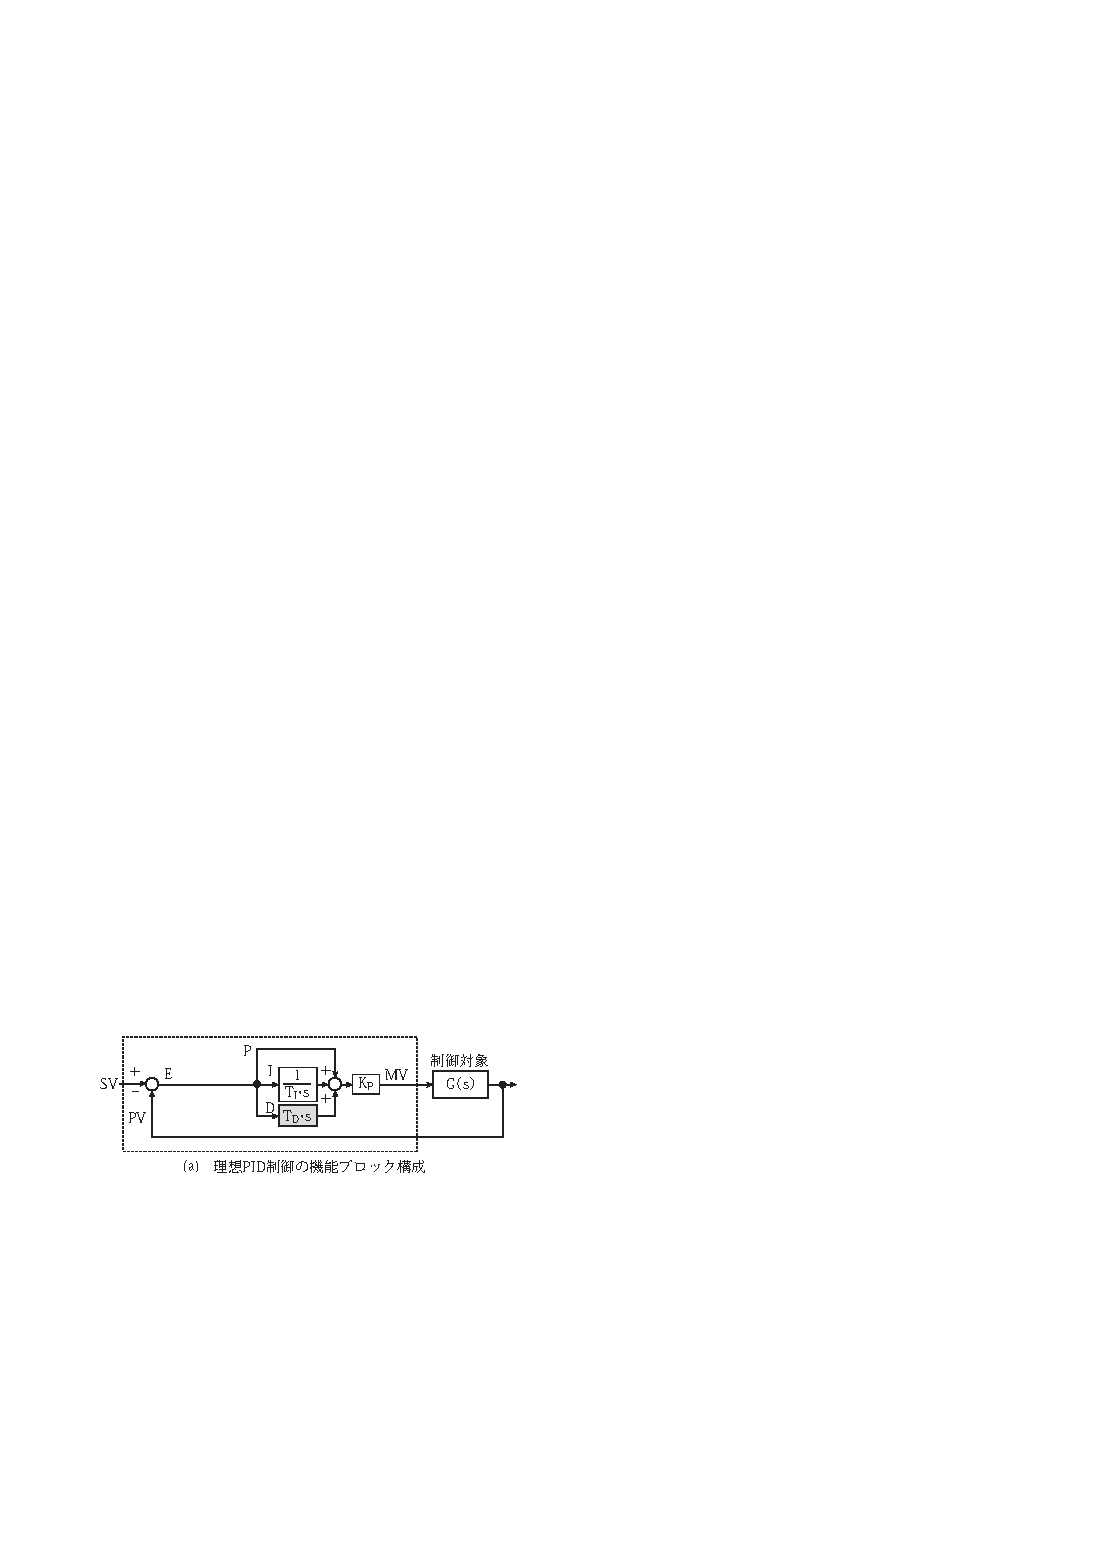
\includegraphics[width=0.8\hsize]{pid_ideal_block.pdf}
  \caption{理想PID制御のブロック図}
  \label{pid_ideal_block}
\end{figure}

\clearpage
理想PID制御の持つ、ノイズに弱いという欠点を解決するために、ノイズを抑制するローパスフィルタ(一次遅れフィルタ)を組み込んだ制御を実用PID制御という。実用PID制御のブロック図を以下の図\ref{pid_practice_block}に示す。
\begin{figure}[htbp]
  \centering
  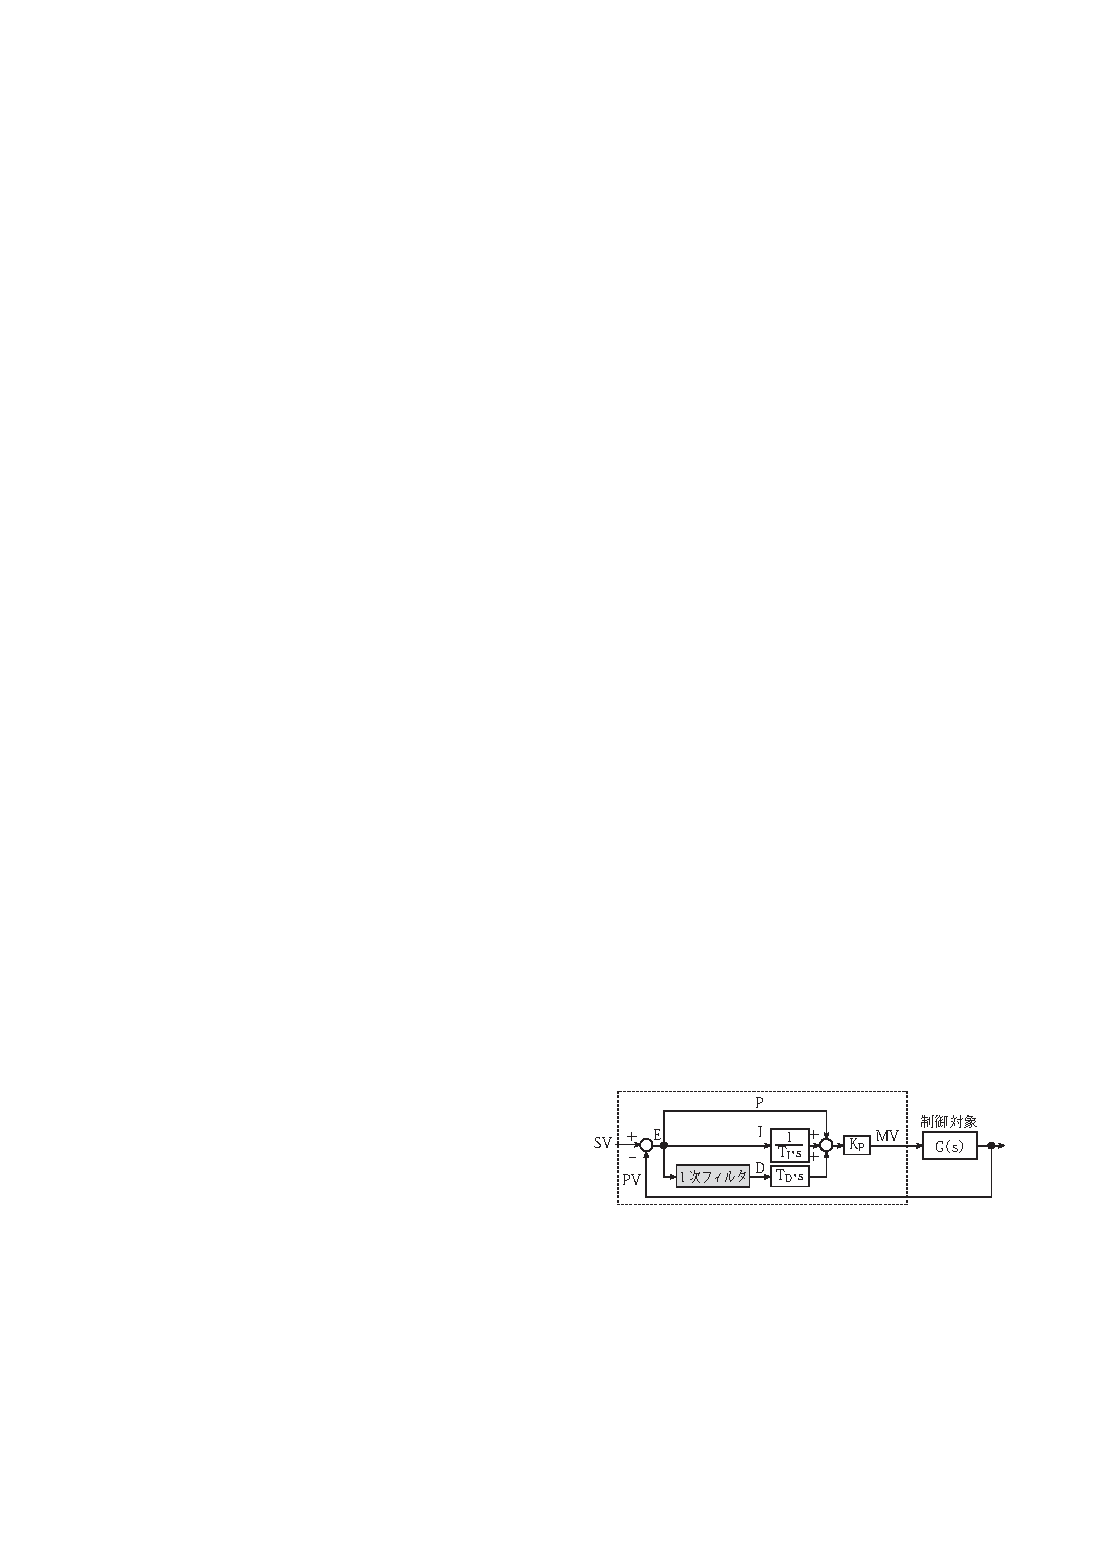
\includegraphics[width=0.8\hsize]{pid_practice_block.pdf}
  \caption{実用PID制御のブロック図}
  \label{pid_practice_block}
\end{figure}
実用PID制御を伝達関数で表現すると、以下の式(\ref{eq:PID_practice4})になり、ブロック図は図\ref{pid_practice_block2}のようになる。このように、フィルタを導入した微分制御のことを不完全微分という。ここで$\eta$は微分係数という定数であり、通常0.1から0.125の値を設定する\cite{実用PIDに向けての工夫その1}
\begin{eqnarray}
  C(t) &=& \frac{U(s)}{E(s)} = K_p \cdot \{1 + \frac{1}{T_i \cdot s}  +  \frac{T_d \cdot s}{1 + \eta \cdot T_d \cdot s}\}
  \label{eq:PID_practice4}
\end{eqnarray}
\begin{figure}[htbp]
  \centering
  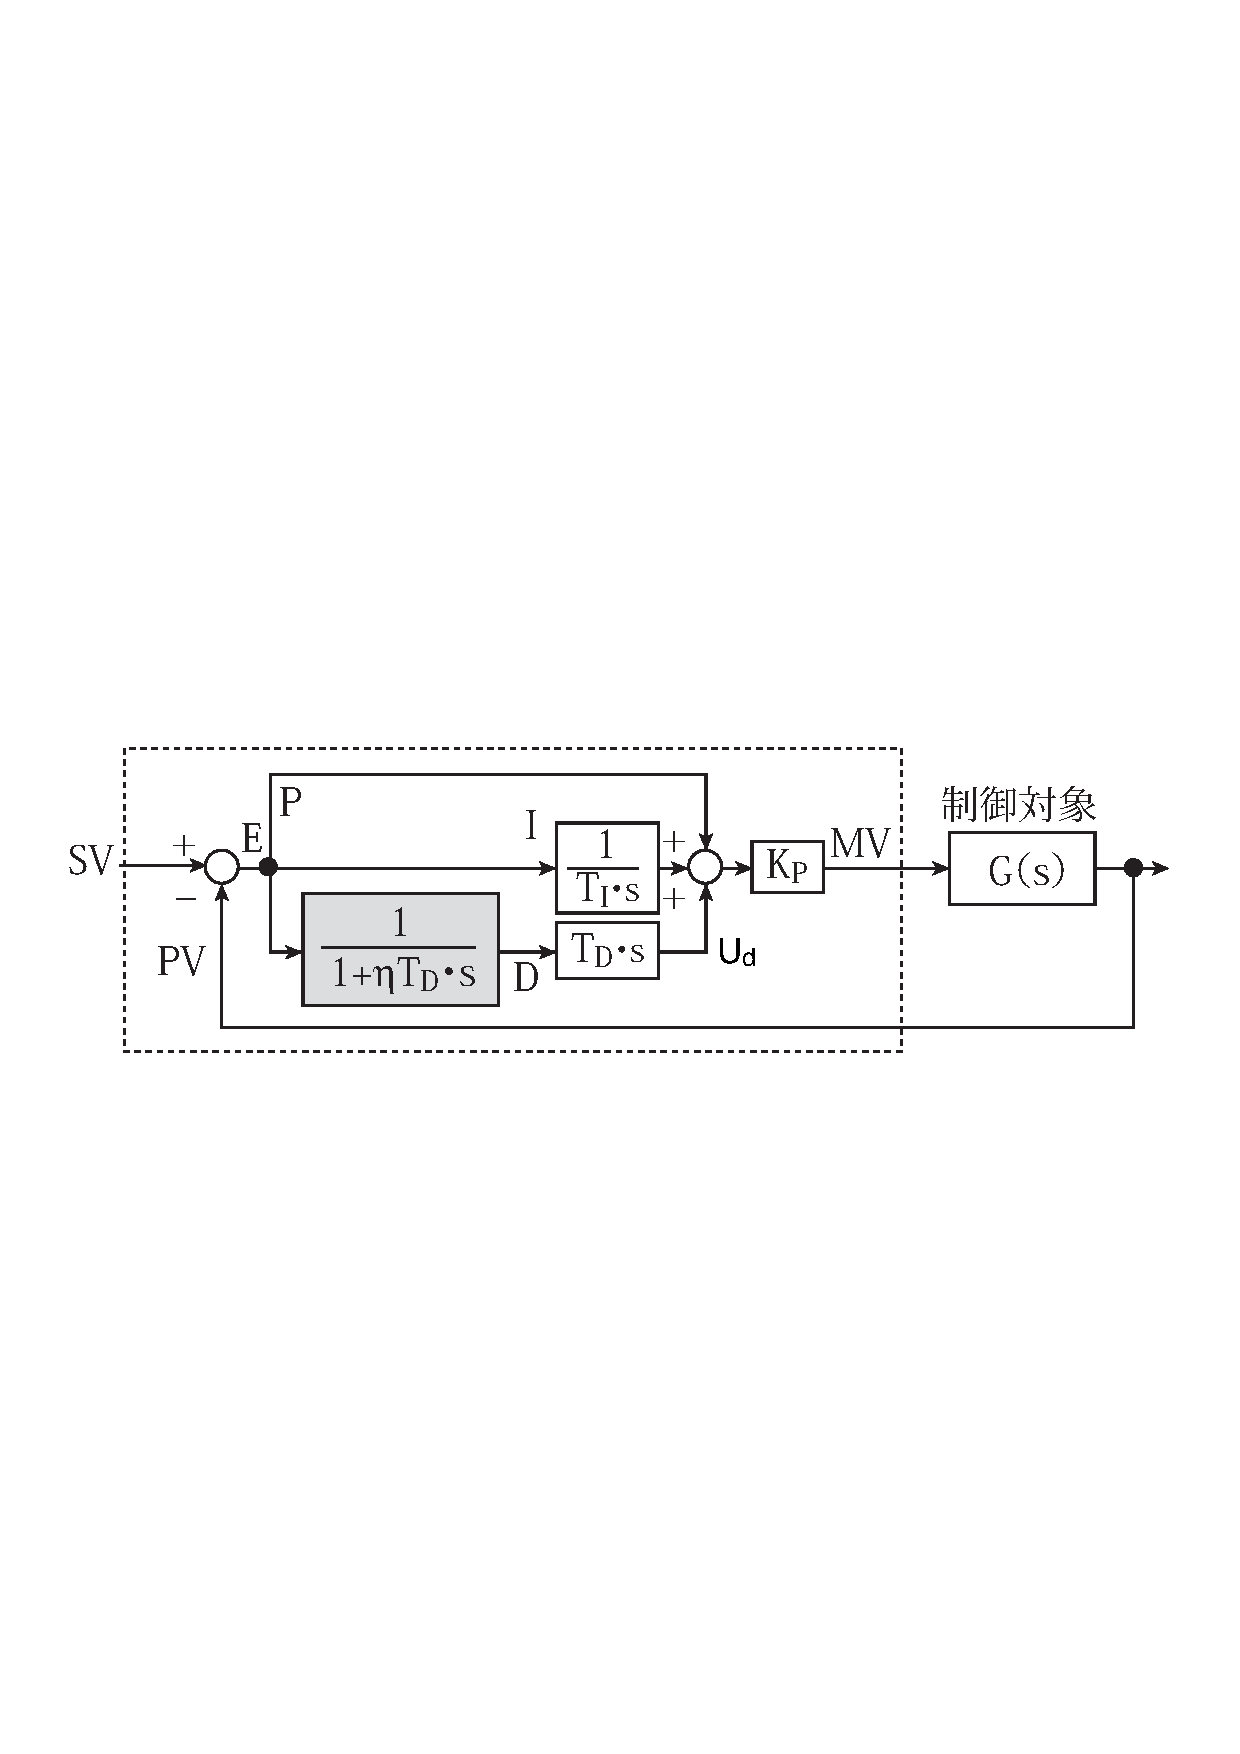
\includegraphics[width=0.8\hsize]{pid_practice_block2.pdf}
  \caption{実用PID制御のブロック図(伝達関数での表現)}
  \label{pid_practice_block2}
\end{figure}


式(\ref{eq:PID_practice4})に示した伝達関数のうち、微分制御に関する部分を抽出した式を以下の式(\ref{eq:D_practice})に示す。
\begin{eqnarray}
  U_d(s) &=& \frac{T_d \cdot s}{1 + \eta \cdot T_d \cdot s} \cdot E(s)
  \label{eq:D_practice}
\end{eqnarray}
式(\ref{eq:D_practice})を式(\ref{eq:D_practice1})のように式変形する。
\begin{eqnarray}
  U_d(s) \cdot (1 + \eta \cdot T_d \cdot s) &=& T_d \cdot s \cdot E(s)\nonumber\\
  U_d(s) + \eta \cdot T_d \cdot s \cdot U_d(s) &=& T_d \cdot s \cdot E(s)
  \label{eq:D_practice1}
\end{eqnarray}
そして、逆ラプラス変換を行うことにより、通常の微分方程式になる(\ref{eq:D_practice2})。
\begin{eqnarray}
  \mathcal{L}^{-1}[U_d(s) + \eta \cdot T_d \cdot s \cdot U_d(s)] &=& \mathcal{L}^{-1}[T_d \cdot s \cdot E(s)]\nonumber\\
  u_d(t) + \eta \cdot T_d \cdot \frac{d}{dt}u_d(t) &=& T_d \cdot \frac{d}{dt}e(t)\nonumber\\
  u_d(t) &=& T_d (\frac{d}{dt}e(t) - \eta \cdot \frac{d}{dt}u_d(t))
  \label{eq:D_practice2}
\end{eqnarray}

以上の議論より、実用PID制御は以下の式で表すことができる。
\begin{eqnarray}
  u(t) &=& K_p \cdot \{e(t) + \frac{1}{T_i} \cdot \int_0^t e(\tau) d\tau +  T_d (\frac{d}{dt}e(t) - \eta \cdot \frac{d}{dt}u_d(t))\}
  \label{eq:PID_practice5}
\end{eqnarray}
\clearpage



\section{移動平均、実用PID制御}
表\ref{table:Ziegler-Nichols_setting}に示したPID制御の値を$K_p$、$K_i$および$K_d$にそれぞれ設定し、シグナリング頻度($s(t)$)を指数移動平均で平滑化した値($\overline{s(t)}$)をPID制御への入力とした場合の評価結果を図\ref{fig:result_pid_average_0-8}、図\ref{fig:result_pid_average_0-1}および図\ref{fig:result_pid_average_0-01}に示す。
\begin{eqnarray}
  \overline{s(t)} &=& \alpha  \cdot s(t) + (1 - \alpha) \cdot \overline{s(t-1)}
  \label{eq:PID_average}
\end{eqnarray}

\begin{figure}[htbp]
 \centering
 \begin{subfigure}{0.49\hsize}
   \centering
   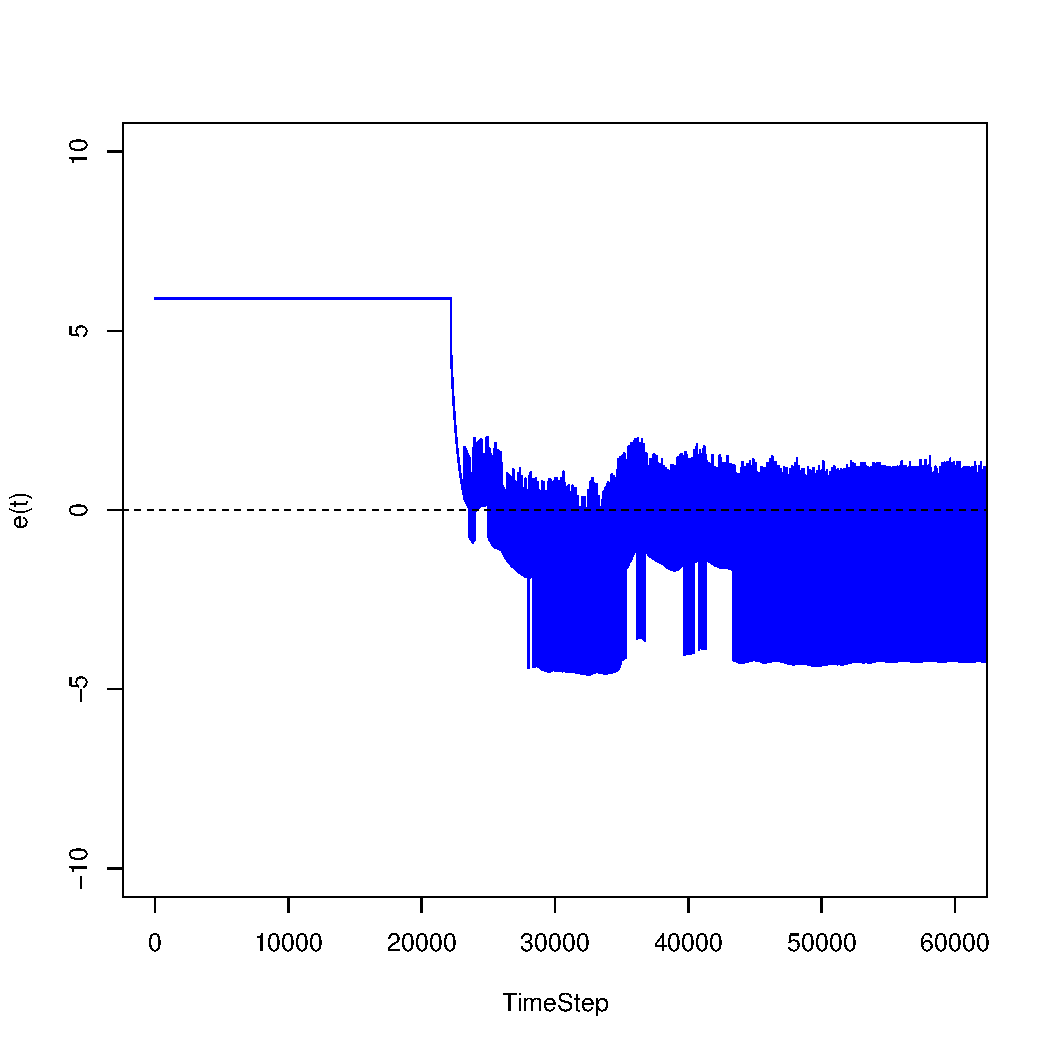
\includegraphics[width=1.0\hsize]{scenario_5_e_86400_345600_1-8_0-00045_1800_0-8_average.pdf}
   \subcaption{$e(t)$の変化}
   \label{subfig:scenario_5_e_86400_345600_0-318_1-8_0-00045_1800_0-8_average}
 \end{subfigure}
 \begin{subfigure}{0.49\hsize}
   \centering
   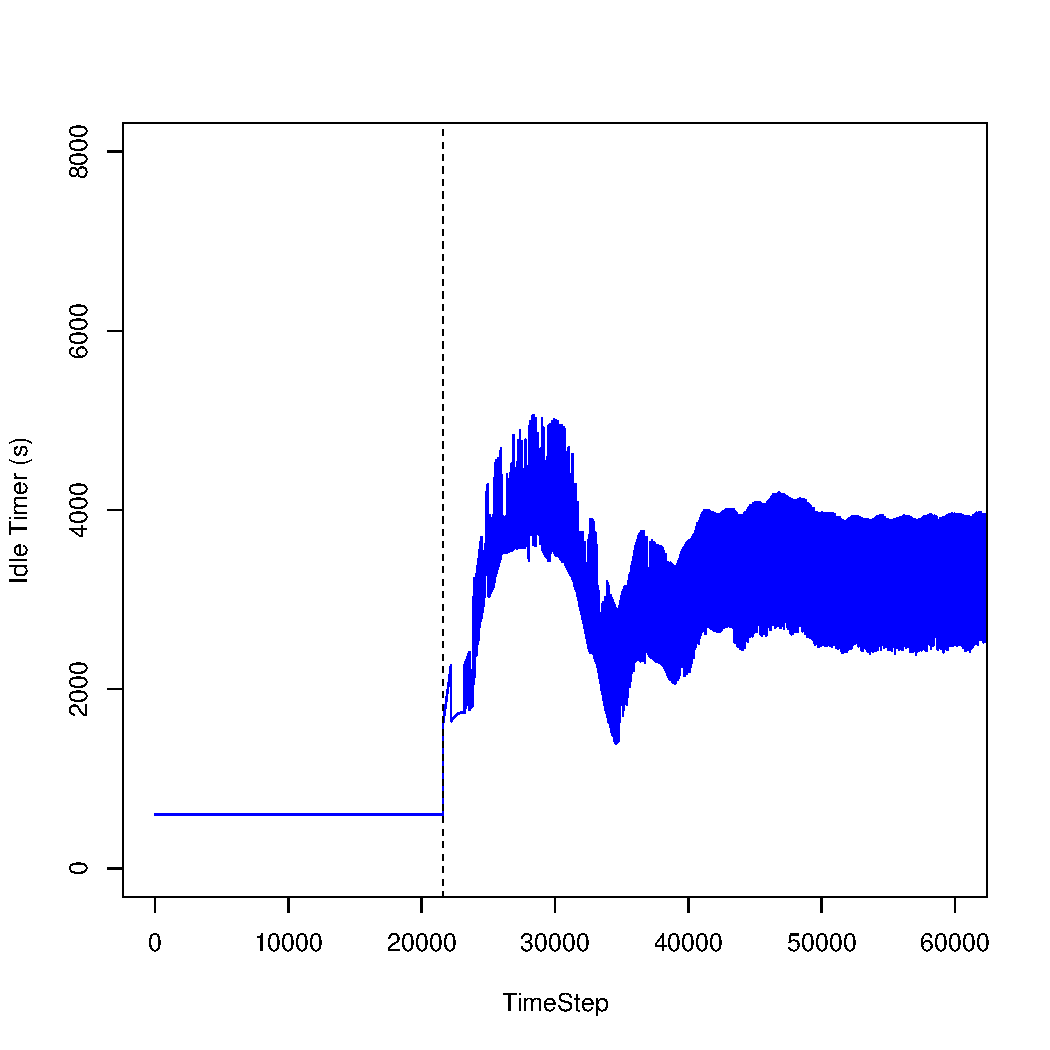
\includegraphics[width=1.0\hsize]{scenario_5_idleTimer_86400_345600_1-8_0-00045_1800_0-8_average.pdf}
   \subcaption{IdleTimerの変化}
   \label{subfig:scenario_5_idleTimer_86400_345600_1-8_0-00045_1800_0-8_average}
 \end{subfigure}
 \par\bigskip %改行
 \begin{subfigure}{0.49\hsize}
   \centering
   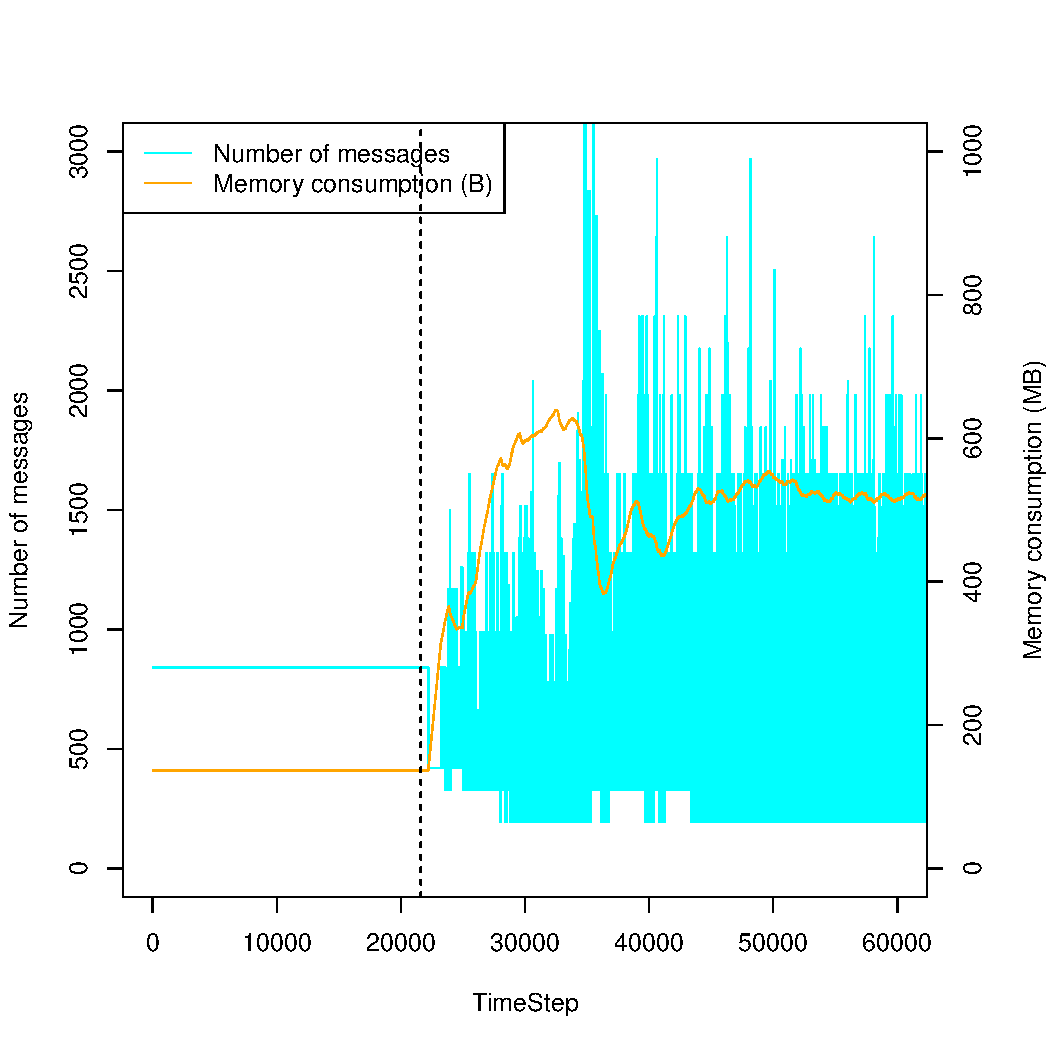
\includegraphics[width=1.0\hsize]{scenario_5_signaling_and_memoryload_vs_timeStep_86400_345600_1-8_0-00045_1800_0-8_average.pdf}
   \subcaption{CPU負荷とメモリ使用量の変化}
   \label{subfig:scenario_5_signaling_and_memoryload_vs_timeStep_86400_345600_1-8_0-00045_1800_0-8_average}
 \end{subfigure}
 \begin{subfigure}{0.49\hsize}
   \centering
   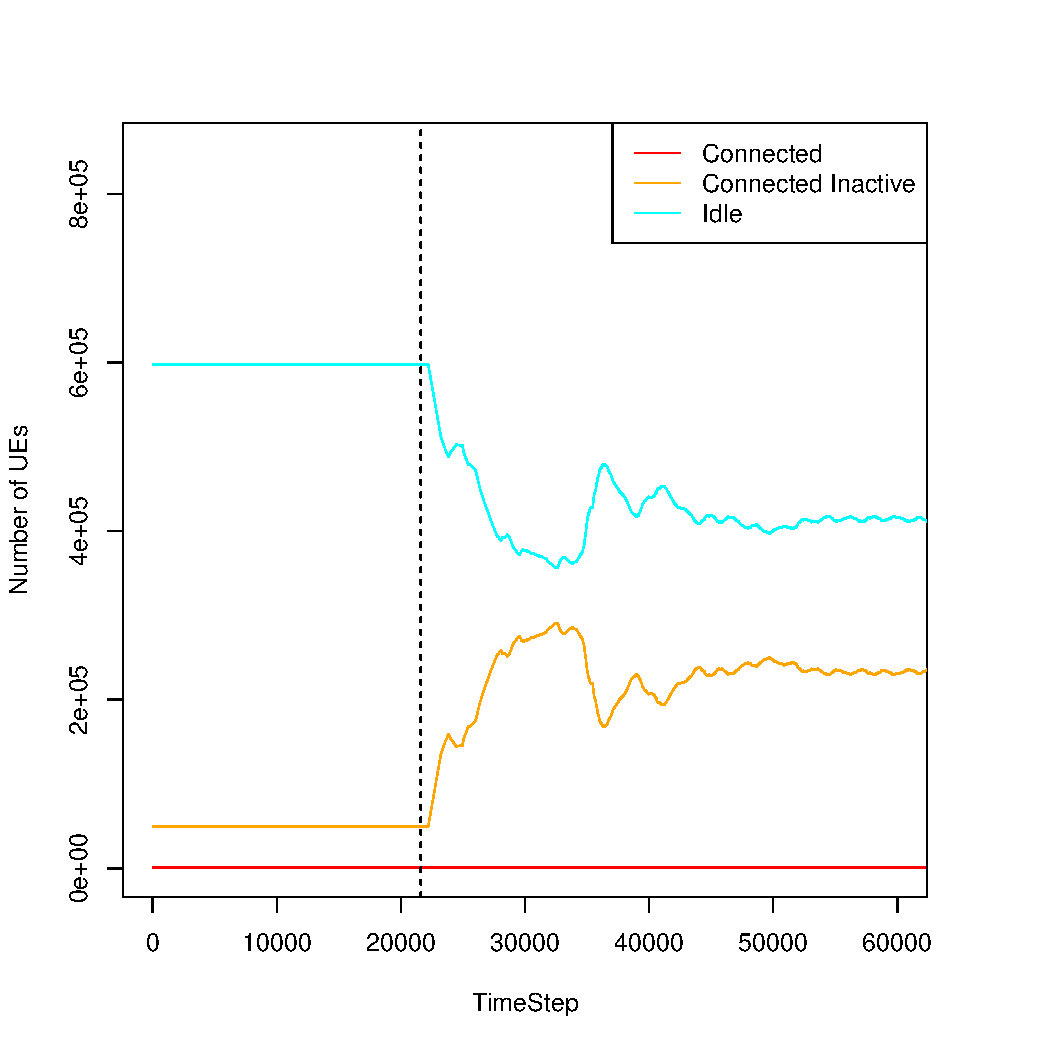
\includegraphics[width=1.0\hsize]{scenario_5_stateBreakdown_86400_345600_1-8_0-00045_1800_0-8_average.pdf}
   \subcaption{各状態にあるUE台数の変化}
   \label{subfig:scenario_5_stateBreakdown_86400_345600_1-8_0-00045_1800_0-8_average}
 \end{subfigure}
 \caption{理想PID($K_p = 1.8、K_i = 0.00045、K_d = 1800、\alpha = 0.8$)}
 \label{fig:result_pid_average_0-8}
\end{figure}
\begin{figure}[htbp]
 \centering
 \begin{subfigure}{0.49\hsize}
   \centering
   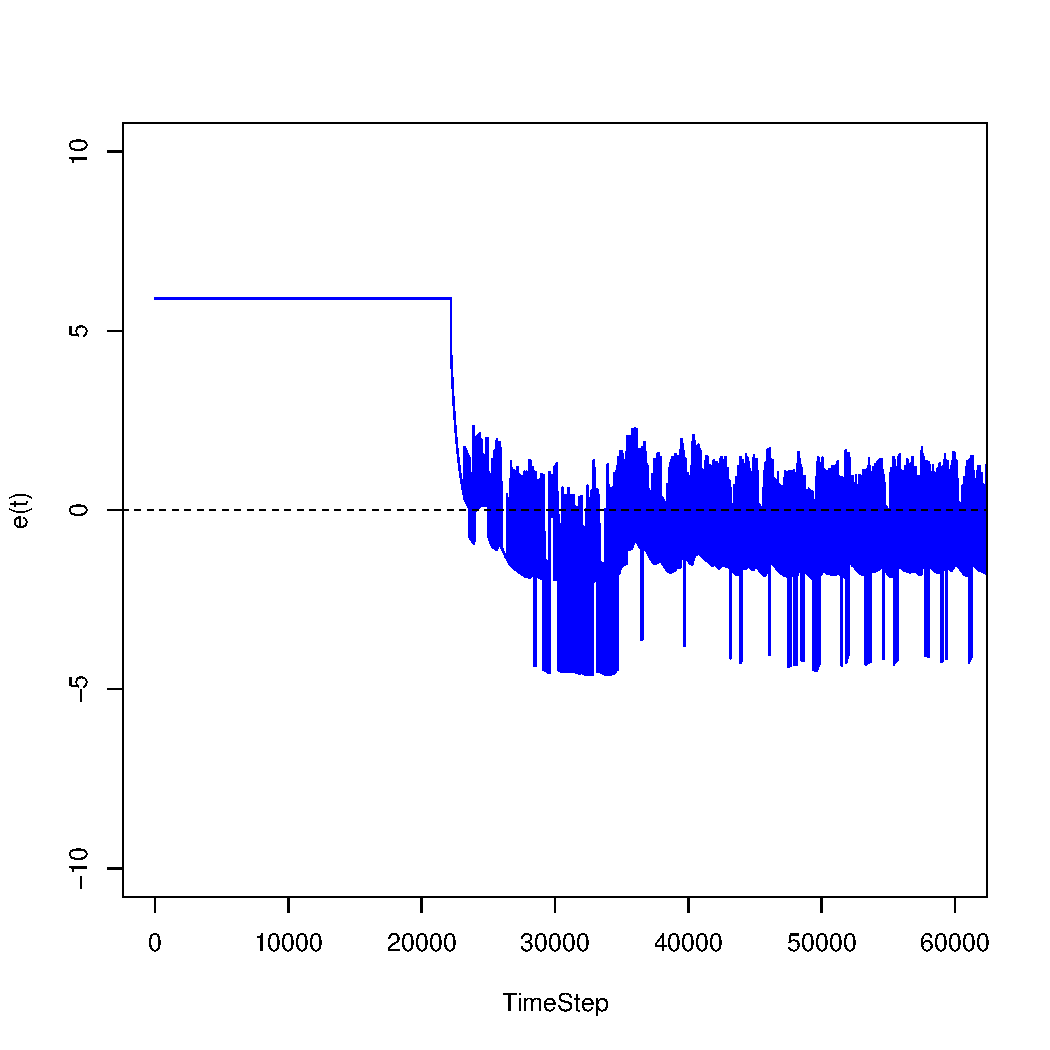
\includegraphics[width=1.0\hsize]{scenario_5_e_86400_345600_1-8_0-00045_1800_0-1_average.pdf}
   \subcaption{$e(t)$の変化}
   \label{subfig:scenario_5_e_86400_345600_0-318_1-8_0-00045_1800_0-1_average}
 \end{subfigure}
 \begin{subfigure}{0.49\hsize}
   \centering
   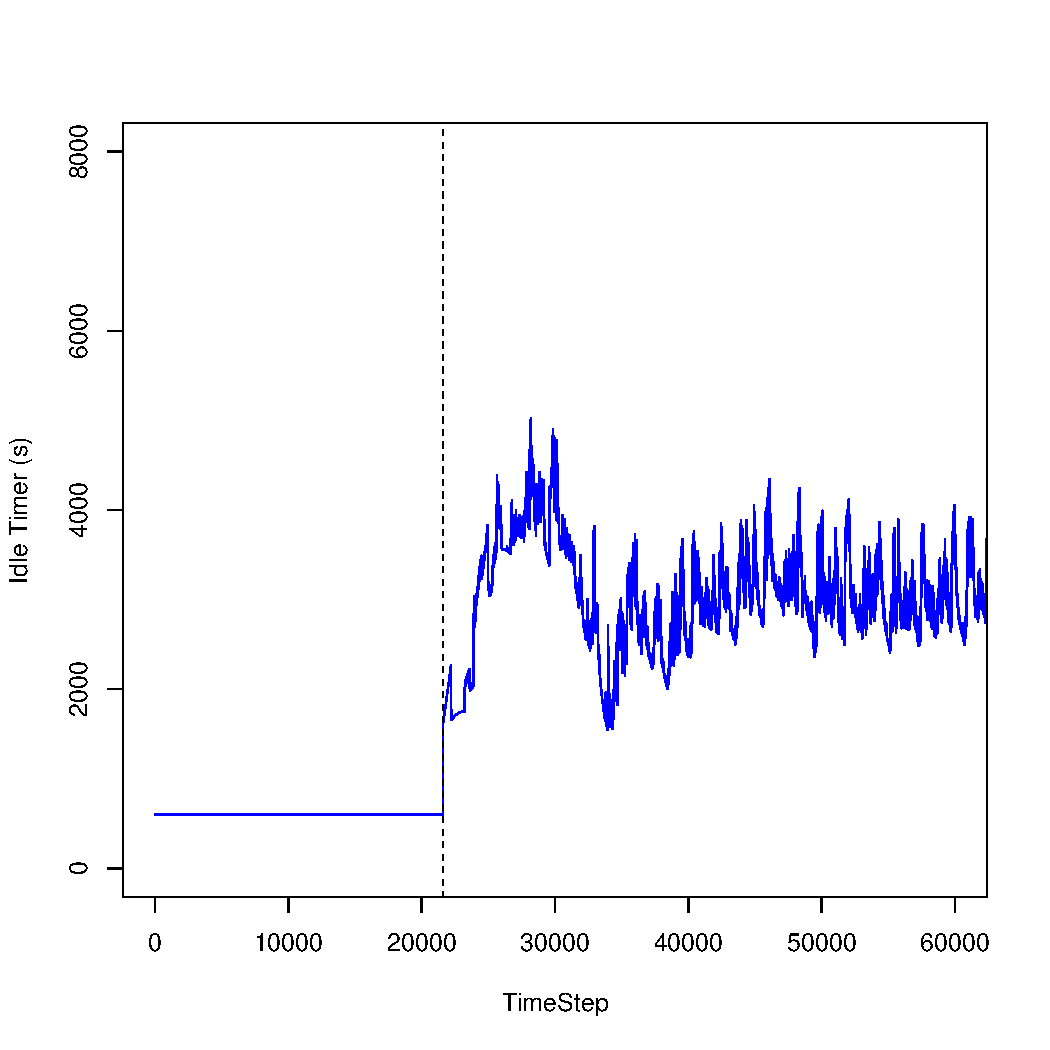
\includegraphics[width=1.0\hsize]{scenario_5_idleTimer_86400_345600_1-8_0-00045_1800_0-1_average.pdf}
   \subcaption{IdleTimerの変化}
   \label{subfig:scenario_5_idleTimer_86400_345600_1-8_0-00045_1800_0-1_average}
 \end{subfigure}
 \par\bigskip %改行
 \begin{subfigure}{0.49\hsize}
   \centering
   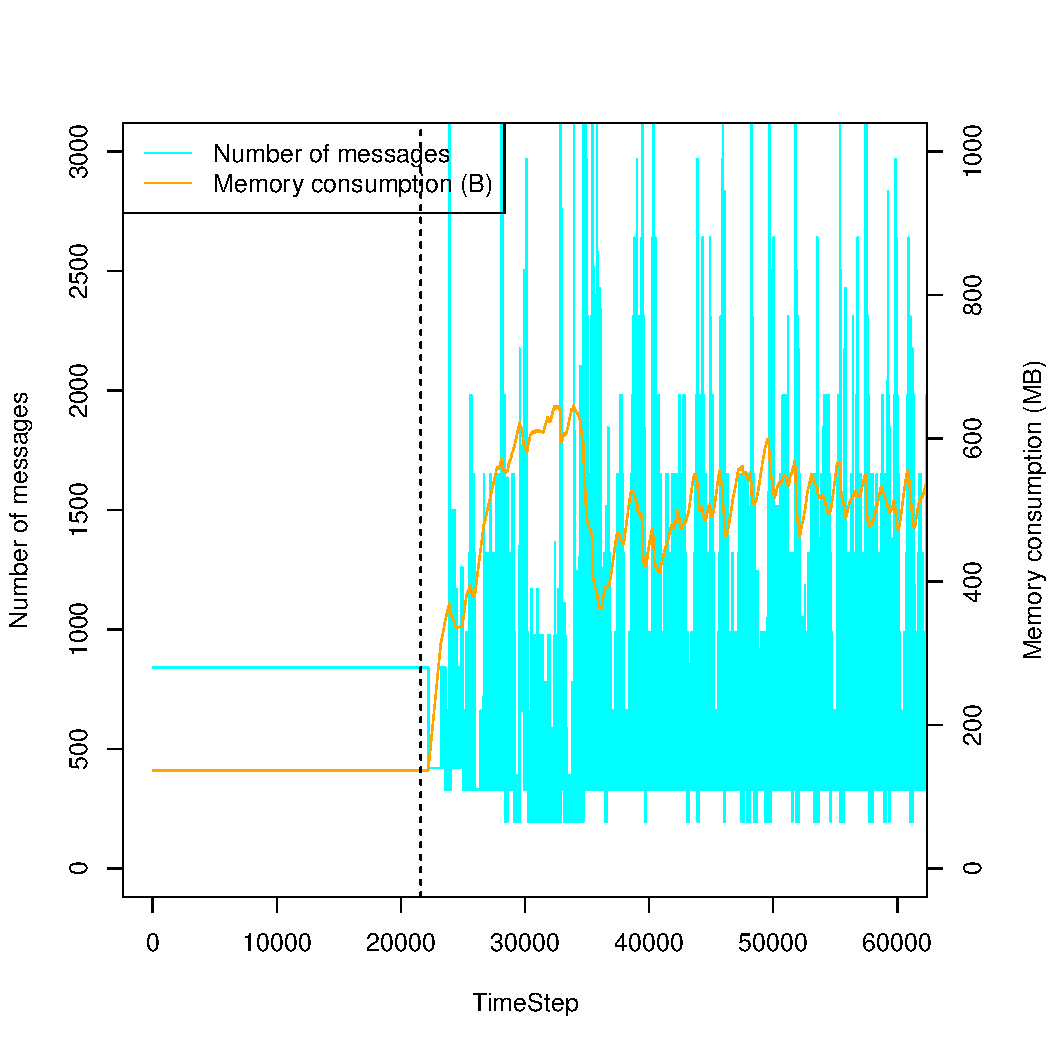
\includegraphics[width=1.0\hsize]{scenario_5_signaling_and_memoryload_vs_timeStep_86400_345600_1-8_0-00045_1800_0-1_average.pdf}
   \subcaption{CPU負荷とメモリ使用量の変化}
   \label{subfig:scenario_5_signaling_and_memoryload_vs_timeStep_86400_345600_1-8_0-00045_1800_0-1_average}
 \end{subfigure}
 \begin{subfigure}{0.49\hsize}
   \centering
   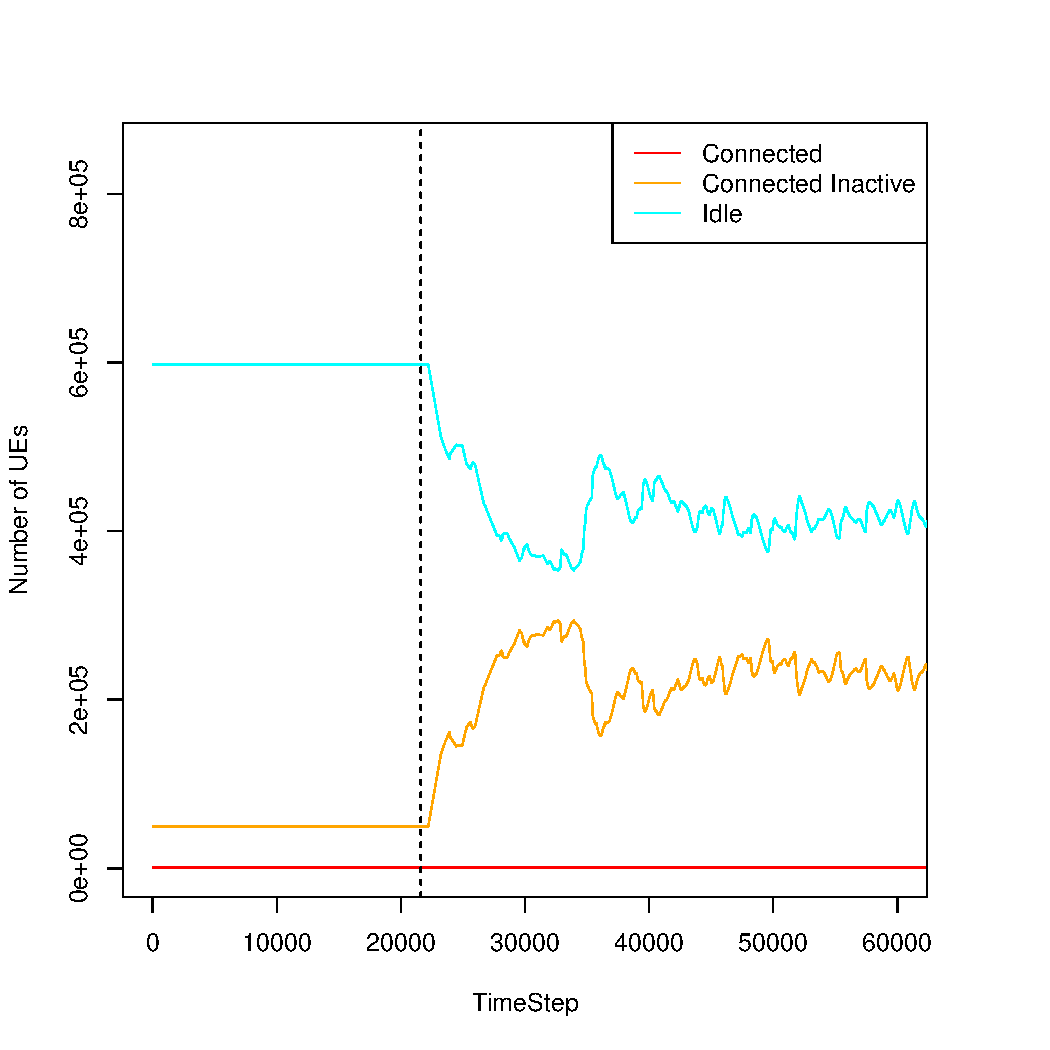
\includegraphics[width=1.0\hsize]{scenario_5_stateBreakdown_86400_345600_1-8_0-00045_1800_0-1_average.pdf}
   \subcaption{各状態にあるUE台数の変化}
   \label{subfig:scenario_5_stateBreakdown_86400_345600_1-8_0-00045_1800_0-1_average}
 \end{subfigure}
 \caption{理想PID($K_p = 1.8、K_i = 0.00045、K_d = 1800、\alpha = 0.1$)}
 \label{fig:result_pid_average_0-1}
\end{figure}
\begin{figure}[htbp]
 \centering
 \begin{subfigure}{0.49\hsize}
   \centering
   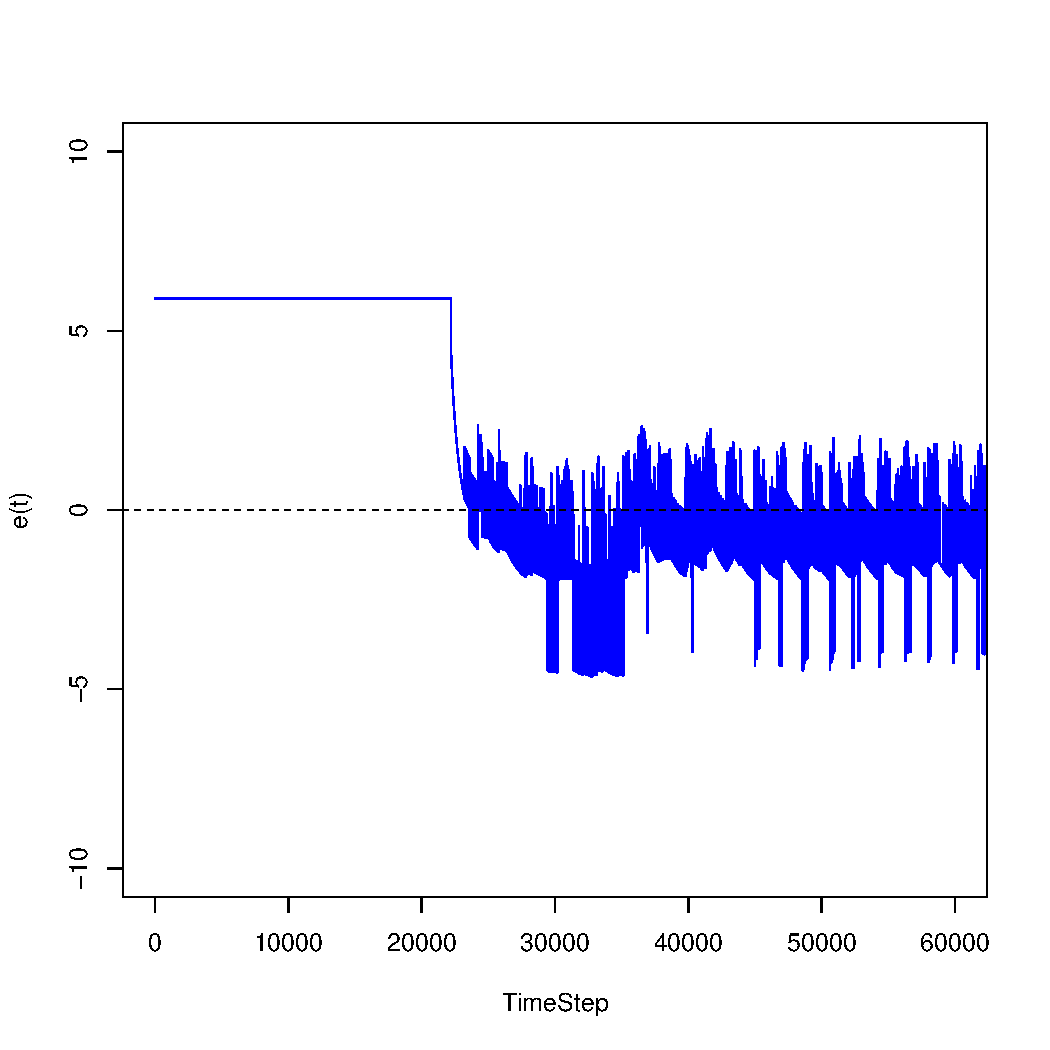
\includegraphics[width=1.0\hsize]{scenario_5_e_86400_345600_1-8_0-00045_1800_0-01_average.pdf}
   \subcaption{$e(t)$の変化}
   \label{subfig:scenario_5_e_86400_345600_0-318_1-8_0-00045_1800_0-01_average}
 \end{subfigure}
 \begin{subfigure}{0.49\hsize}
   \centering
   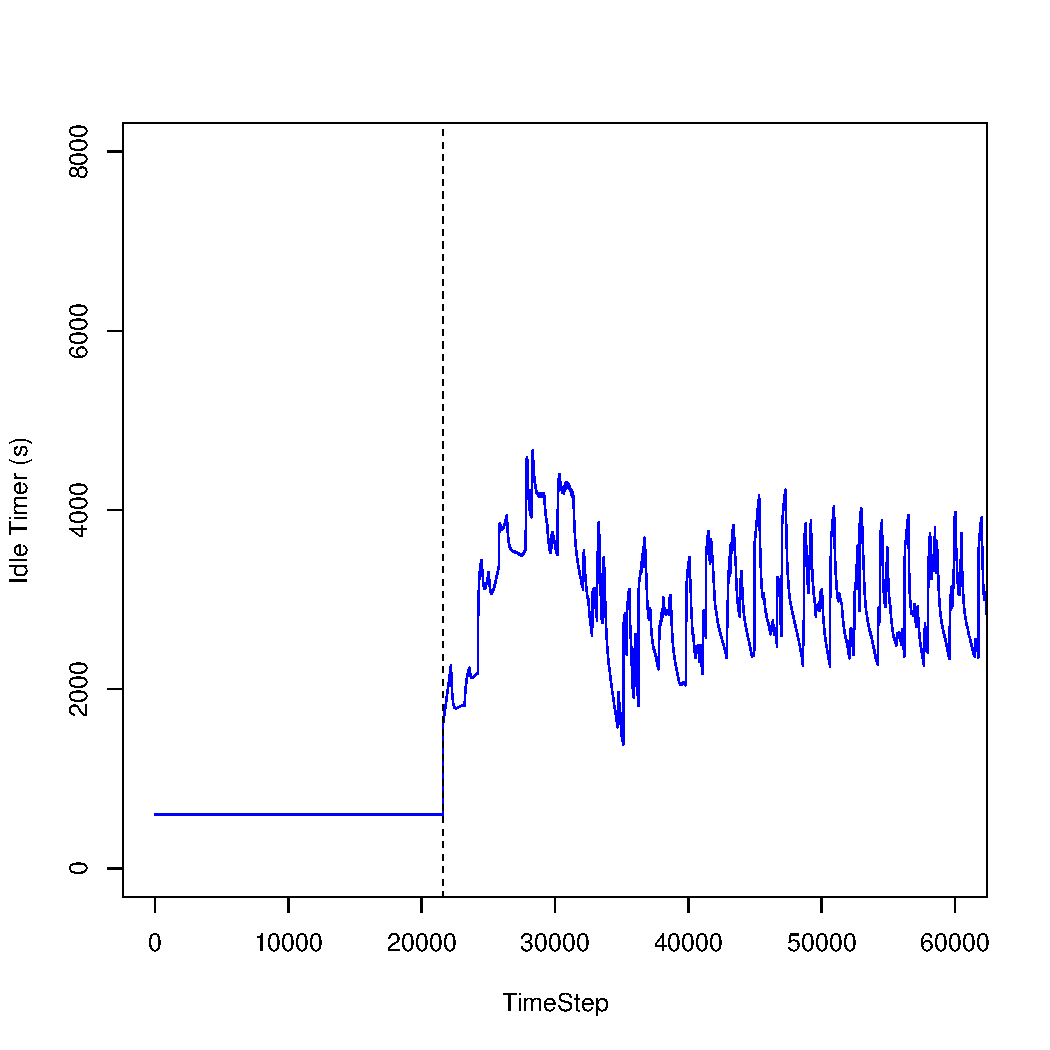
\includegraphics[width=1.0\hsize]{scenario_5_idleTimer_86400_345600_1-8_0-00045_1800_0-01_average.pdf}
   \subcaption{IdleTimerの変化}
   \label{subfig:scenario_5_idleTimer_86400_345600_1-8_0-00045_1800_0-01_average}
 \end{subfigure}
 \par\bigskip %改行
 \begin{subfigure}{0.49\hsize}
   \centering
   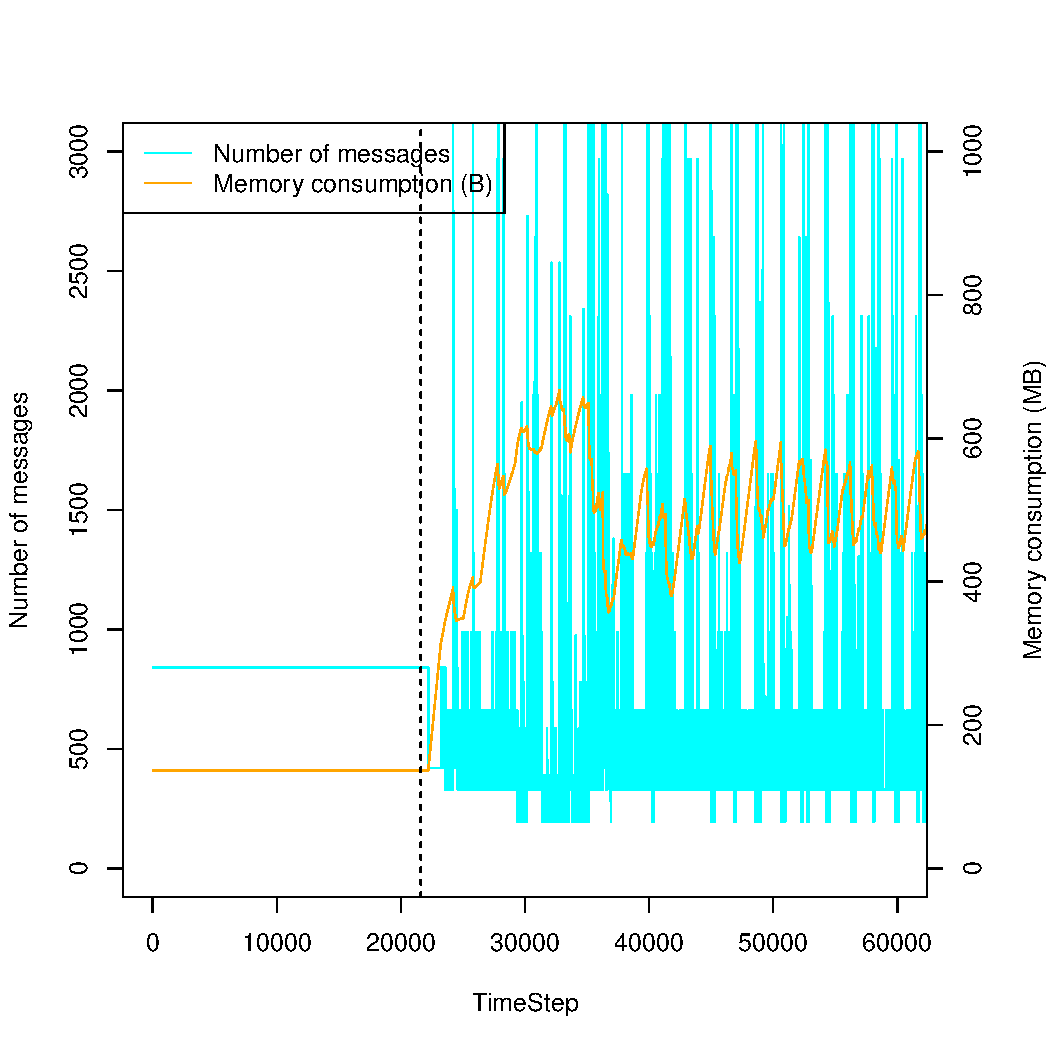
\includegraphics[width=1.0\hsize]{scenario_5_signaling_and_memoryload_vs_timeStep_86400_345600_1-8_0-00045_1800_0-01_average.pdf}
   \subcaption{CPU負荷とメモリ使用量の変化}
   \label{subfig:scenario_5_signaling_and_memoryload_vs_timeStep_86400_345600_1-8_0-00045_1800_0-01_average}
 \end{subfigure}
 \begin{subfigure}{0.49\hsize}
   \centering
   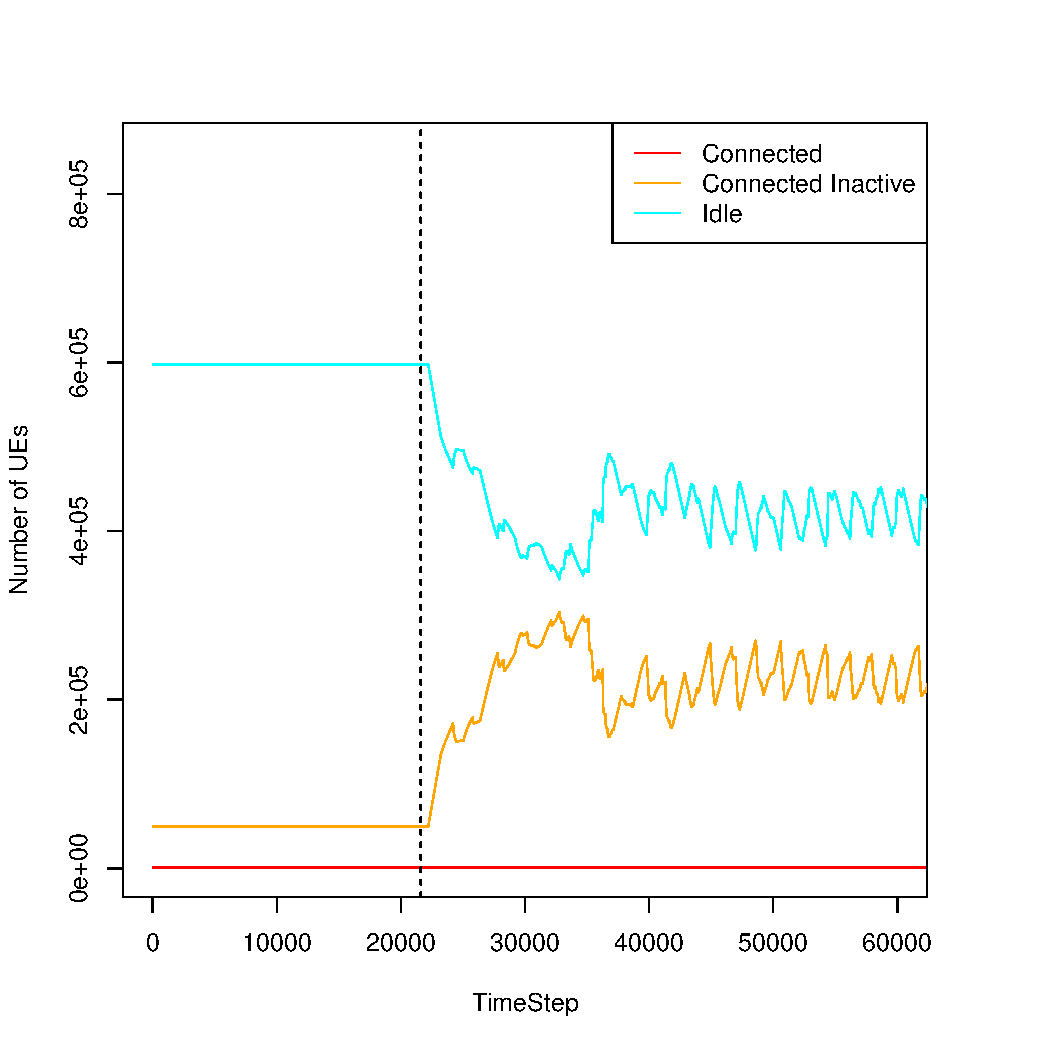
\includegraphics[width=1.0\hsize]{scenario_5_stateBreakdown_86400_345600_1-8_0-00045_1800_0-01_average.pdf}
   \subcaption{各状態にあるUE台数の変化}
   \label{subfig:scenario_5_stateBreakdown_86400_345600_1-8_0-00045_1800_0-01_average}
 \end{subfigure}
 \caption{理想PID($K_p = 1.8、K_i = 0.00045、K_d = 1800、\alpha = 0.01$)}
 \label{fig:result_pid_average_0-01}
\end{figure}


\clearpage
表\ref{table:Ziegler-Nichols_setting}に示したPID制御の値を$K_p$、$K_i$および$K_d$にそれぞれ設定し、不完全微分を用いた実用PID制御を行った場合の評価結果を図\ref{fig:result_pid_practice_0-125}、図\ref{fig:result_pid_practice_0-5}および図\ref{fig:result_pid_practice_0-8}に示す。
\begin{figure}[htbp]
  \begin{center}
    \begin{tabular}{c}
      \begin{minipage}{0.45\hsize}
        \begin{center}
        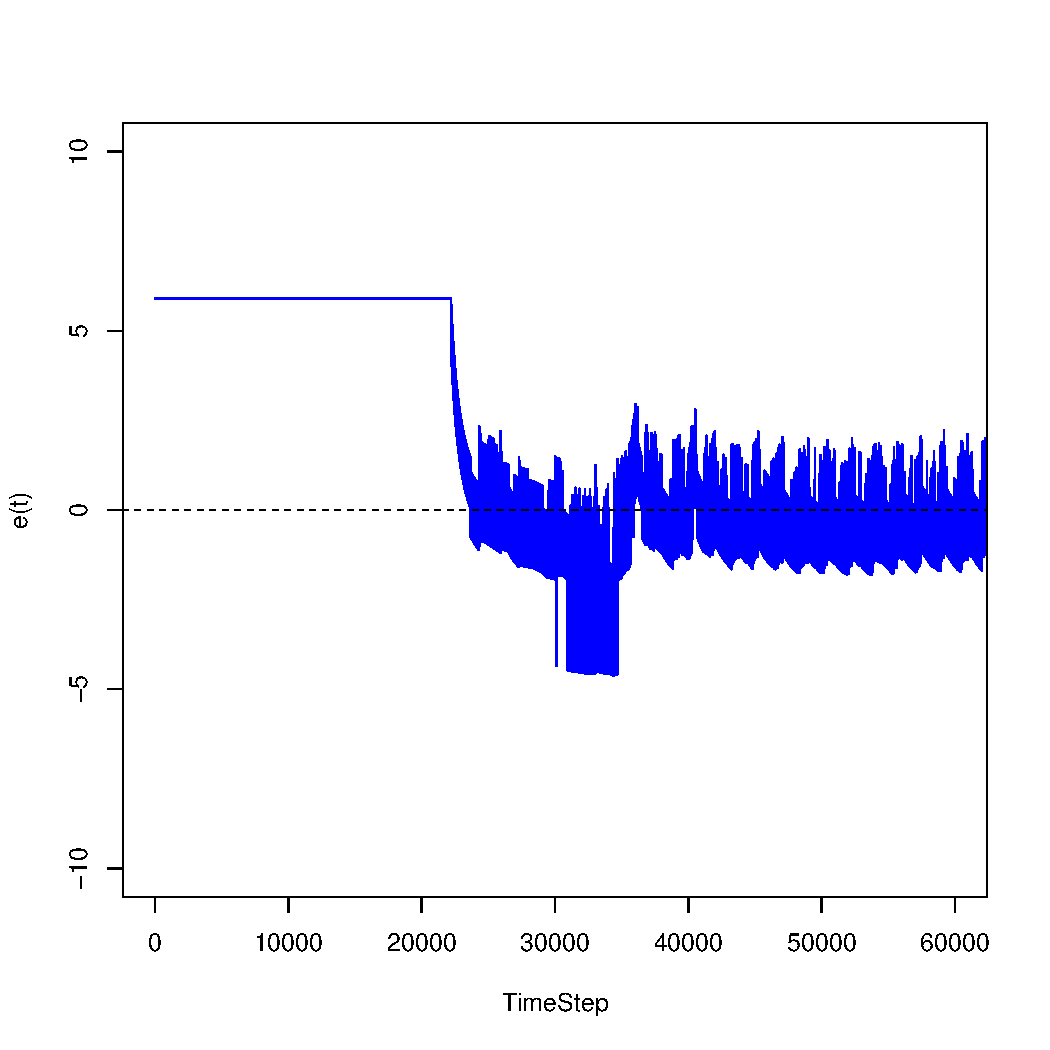
\includegraphics[width=1\hsize]{scenario_5_e_86400_345600_1-8_0-00045_1800_0-125_practice.pdf}
        \subcaption{$e(t)$の変化}
        \label{scenario_5_e_86400_345600_0-318_1-8_0-00045_1800_0-125_practice}
        \end{center}
      \end{minipage}
      \begin{minipage}{0.45\hsize}
        \begin{center}
        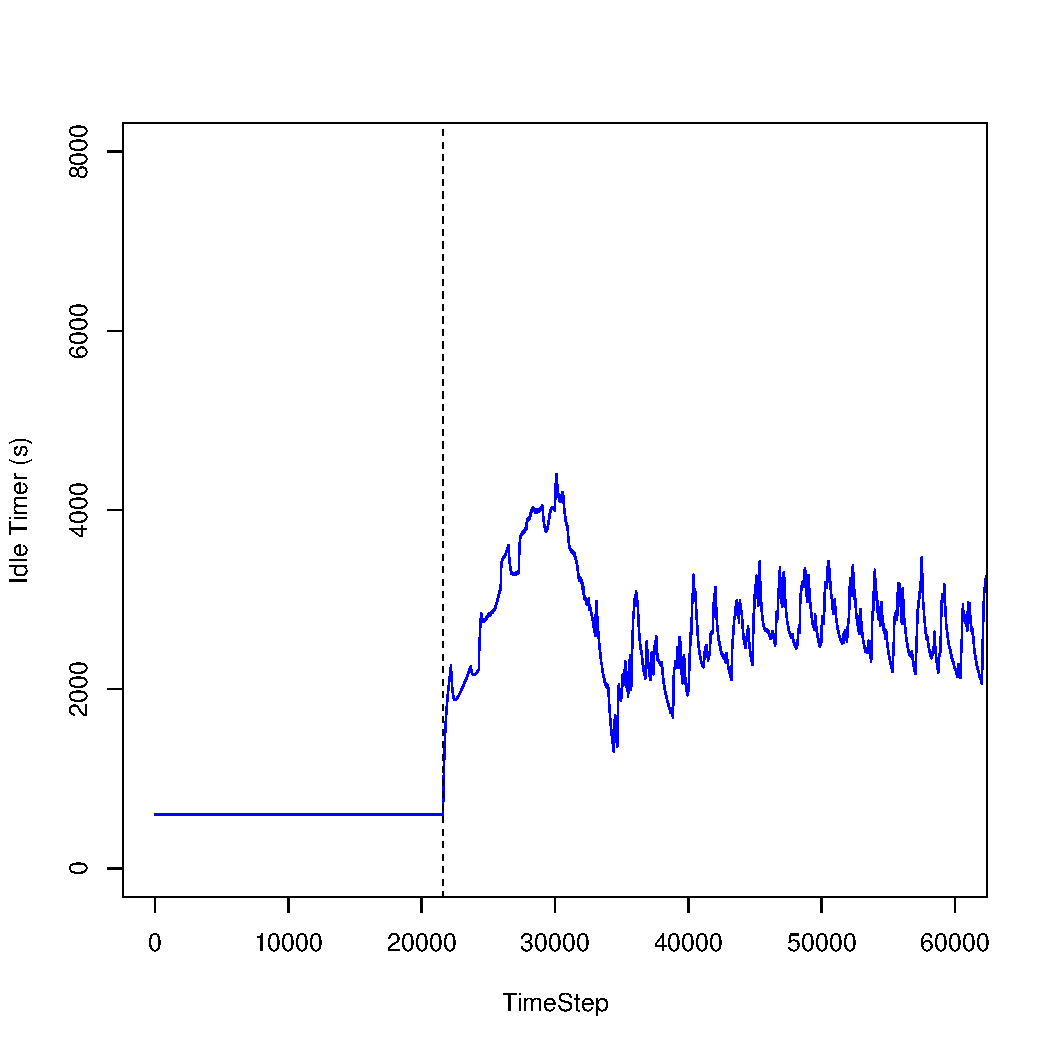
\includegraphics[width=1\hsize]{scenario_5_idleTimer_86400_345600_1-8_0-00045_1800_0-125_practice.pdf}
        \subcaption{IdleTimerの変化}
        \label{scenario_5_idleTimer_86400_345600_1-8_0-00045_1800_0-125_practice}
        \end{center}
      \end{minipage}\\
      \begin{minipage}{0.45\hsize}
        \begin{center}
        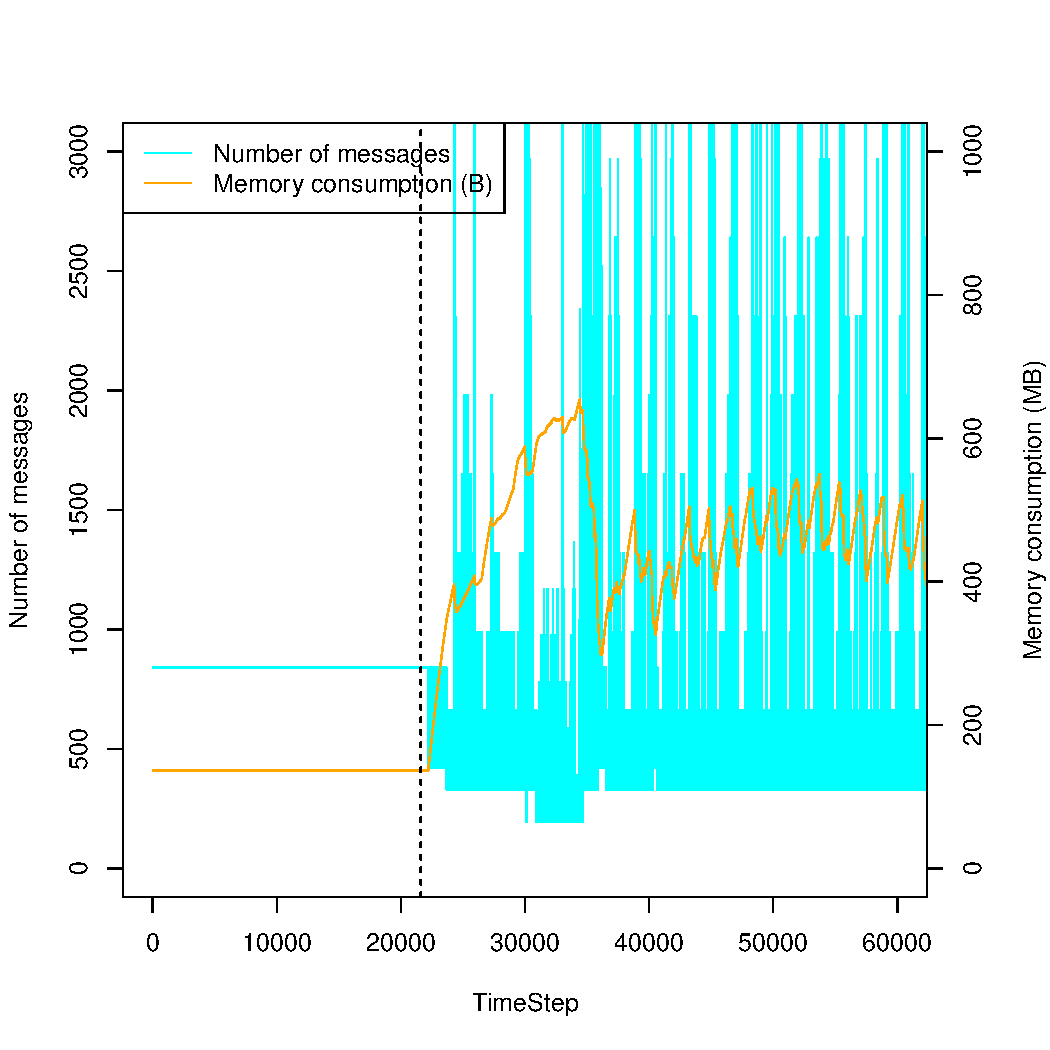
\includegraphics[width=1\hsize]{scenario_5_signaling_and_memoryload_vs_timeStep_86400_345600_1-8_0-00045_1800_0-125_practice.pdf}
        \subcaption{CPU負荷とメモリ使用量の変化}
        \label{scenario_5_signaling_and_memoryload_vs_timeStep_86400_345600_1-8_0-00045_1800_0-125_practice}
        \end{center}
      \end{minipage}
      \begin{minipage}{0.45\hsize}
        \begin{center}
        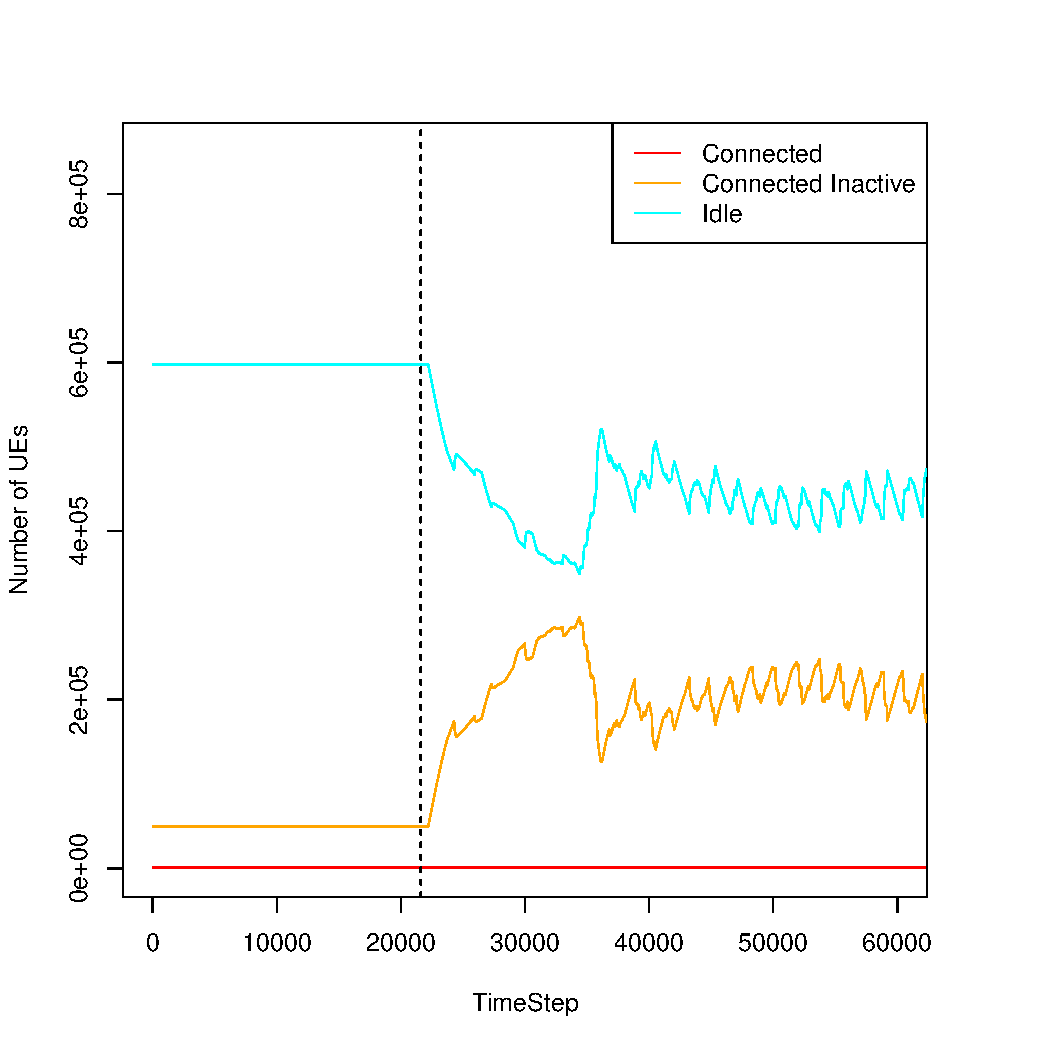
\includegraphics[width=1\hsize]{scenario_5_stateBreakdown_86400_345600_1-8_0-00045_1800_0-125_practice.pdf}
        \subcaption{各状態にあるUE台数の変化}
        \label{scenario_5_stateBreakdown_86400_345600_1-8_0-00045_1800_0-125_practice}
        \end{center}
      \end{minipage}
    \end{tabular}
    \caption{実用PID($K_p = 1.8、K_i = 0.00045、K_d = 1800、\eta = 0.125$)}
    \label{fig:result_pid_practice_0-125}
  \end{center}
\end{figure}
\begin{figure}[htbp]
  \begin{center}
    \begin{tabular}{c}
      \begin{minipage}{0.45\hsize}
        \begin{center}
        \includegraphics[width=1\hsize]{scenario_5_e_86400_345600_1-8_0-00045_1800_0-5_practice.pdf}
        \subcaption{$e(t)$の変化}
        \label{scenario_5_e_86400_345600_0-318_1-8_0-00045_1800_0-5_practice}
        \end{center}
      \end{minipage}
      \begin{minipage}{0.45\hsize}
        \begin{center}
        \includegraphics[width=1\hsize]{scenario_5_idleTimer_86400_345600_1-8_0-00045_1800_0-5_practice.pdf}
        \subcaption{IdleTimerの変化}
        \label{scenario_5_idleTimer_86400_345600_1-8_0-00045_1800_0-5_practice}
        \end{center}
      \end{minipage}\\
      \begin{minipage}{0.45\hsize}
        \begin{center}
        \includegraphics[width=1\hsize]{scenario_5_signaling_and_memoryload_vs_timeStep_86400_345600_1-8_0-00045_1800_0-5_practice.pdf}
        \subcaption{CPU負荷とメモリ使用量の変化}
        \label{scenario_5_signaling_and_memoryload_vs_timeStep_86400_345600_1-8_0-00045_1800_0-5_practice}
        \end{center}
      \end{minipage}
      \begin{minipage}{0.45\hsize}
        \begin{center}
        \includegraphics[width=1\hsize]{scenario_5_stateBreakdown_86400_345600_1-8_0-00045_1800_0-5_practice.pdf}
        \subcaption{各状態にあるUE台数の変化}
        \label{scenario_5_stateBreakdown_86400_345600_1-8_0-00045_1800_0-5_practice}
        \end{center}
      \end{minipage}
    \end{tabular}
    \caption{実用PID($K_p = 1.8、K_i = 0.00045、K_d = 1800、\eta = 0.5$)}
    \label{fig:result_pid_practice_0-5}
  \end{center}
\end{figure}
\begin{figure}[htbp]
  \begin{center}
    \begin{tabular}{c}
      \begin{minipage}{0.45\hsize}
        \begin{center}
        \includegraphics[width=1\hsize]{scenario_5_e_86400_345600_1-8_0-00045_1800_0-8_practice.pdf}
        \subcaption{$e(t)$の変化}
        \label{scenario_5_e_86400_345600_0-318_1-8_0-00045_1800_0-8_practice}
        \end{center}
      \end{minipage}
      \begin{minipage}{0.45\hsize}
        \begin{center}
        \includegraphics[width=1\hsize]{scenario_5_idleTimer_86400_345600_1-8_0-00045_1800_0-8_practice.pdf}
        \subcaption{IdleTimerの変化}
        \label{scenario_5_idleTimer_86400_345600_1-8_0-00045_1800_0-8_practice}
        \end{center}
      \end{minipage}\\
      \begin{minipage}{0.45\hsize}
        \begin{center}
        \includegraphics[width=1\hsize]{scenario_5_signaling_and_memoryload_vs_timeStep_86400_345600_1-8_0-00045_1800_0-8_practice.pdf}
        \subcaption{CPU負荷とメモリ使用量の変化}
        \label{scenario_5_signaling_and_memoryload_vs_timeStep_86400_345600_1-8_0-00045_1800_0-8_practice}
        \end{center}
      \end{minipage}
      \begin{minipage}{0.45\hsize}
        \begin{center}
        \includegraphics[width=1\hsize]{scenario_5_stateBreakdown_86400_345600_1-8_0-00045_1800_0-8_practice.pdf}
        \subcaption{各状態にあるUE台数の変化}
        \label{scenario_5_stateBreakdown_86400_345600_1-8_0-00045_1800_0-8_practice}
        \end{center}
      \end{minipage}
    \end{tabular}
    \caption{実用PID($K_p = 1.8、K_i = 0.00045、K_d = 1800、\eta = 0.8$)}
    \label{fig:result_pid_practice_0-8}
  \end{center}
\end{figure}


\clearpage
以上の結果より、指数移動平均や実用PID制御を用いて入力の離散的な変動を平滑化することによって、そのような制御を行わない場合(図\ref{fig:result_pid})と比較して制御が安定することがわかる。
しかし、依然としてIdleタイマの制御が十分安定しているとは言えない。

指数移動平均を用いた結果を見ると、$\alpha$の値が小さい場合、短い周期でのIdleタイマが変動が安定することがわかる。
一方で、オーバシュートの発生により、周期の大きな変動が発生していることがわかる。

同様に、実用PID制御を用いた結果を見ると、微分係数$\eta$の値が大きい場合、短い周期でのIdleタイマの変動を抑制できることがわかる。
一方で、オーバシュートの発生により、周期の大きな変動が発生していることがわかる。


% \begin{comment}
図\ref{result_pid_average}に示したIdleタイマの変化とシグナリング頻度の変化をタイムステップ50,000から55,000の範囲でプロットしたグラフを図\ref{scenario_5_analyze_86400_345600_0-318_3725_931-25_0-125_average}に示す。
この図を見ると、Idleタイマおよびシグナリング頻度は周期的に変動していることがわかる。
また、それぞれの変動のタイミングおよび周期が一致していることもわかる。
これは、シグナリング頻度の変化にIdleタイマを追従させるようにPID制御が機能しているためである。
シグナリング頻度が周期的に変化している理由は、Idleタイマの変化によって、UEの状態遷移が集中する期間が周期的に発生するためである。
図中の左側に2本の破線と2本の直線を引いた。2本の破線に囲まれた期間はシグナリング頻度が大きく、Idleタイマが約3,500~sに設定されている。
一方、2本の直線に囲まれた期間はシグナリング頻度が小さく、Idleタイマは約3,100~sに設定されている。
すると、破線で示した期間にデータ送信を行ったUEは、約3,500~s後にConnected Inactive 状態からアイドル状態への状態遷移を発生させる。
同様に、直線で示した期間にデータ送信を行ったUEは、約3,100~s後に状態遷移を発生させる。このタイミングを図中の右側の破線および直線に示す。
右側の破線および直線は左側の破線および直線のそれぞれ3,500~s、3,100~s後を示している。
これを見ると、UEの状態遷移のタイミングが重なっていることがわかる。
また、それが原因となり、シグナリング頻度が大きくなっている。
上述のように、シグナリング頻度の変動が、一定期間後に同様のシグナリング頻度の変動を引き起こす場合がある。
\begin{figure}[htbp]
  \centering
    \includegraphics[width=1\hsize]{scenario_5_analyze_86400_345600_0-318_3725_931-25_0-125_average.pdf}
    \caption{IdleタイマとCPU負荷の変化($K_p = 0.318、K_i = 0.0000854、K_d = 296.14$、移動平均)}
    \label{scenario_5_analyze_86400_345600_0-318_3725_931-25_0-125_average}
\end{figure}
% \end{comment}


\clearpage
\section{制御の性質}
\begin{description}
  \item[比例制御] 比例ゲインが小さい場合は制御が収束するまでにかかる時間が増加し、比例ゲインが大きい場合はオーバーシュートやハンチング等が発生して制御が不安定になる(一般的な性質)。
  \item[積分制御] 一般的に積分ゲインは定常偏差を抑制するために有効であるが、本評価では定常偏差が発生しないため、積分制御の効果は限定的であると言える。
  \item[微分制御] 微分制御により、過渡応答特性を改善することが可能である(一般的な性質)。一方で、本評価では、離散的な負荷の変動が発生しているため、制御が不安的になる。
  \item[指数移動平均を用いた制御] 指数移動平均を用いることで離散的な負荷の変動を平滑化して、制御を安定させることが可能である。制御の安定性と、変動に対する応答性はトレードオフの関係がある。平滑化係数の値を小さくすると離散的な負荷の変動を平滑化できるが、オーバーシュートやハンチングが発生しやすくなる。
  \item[実用PID制御] 不完全微分を用いることで、一時的な負荷の変動を平滑化して制御を安定させることが可能である。制御の安定性と、変動に対する応答性はトレードオフの関係がある。微分係数の値を大きくすると、一時的な負荷の変動を平滑化できるが、過渡応答特性が低下する。
\end{description}

\section{異なるシナリオでの評価}
UE台数は480,000台であり、UEの持つ通信周期とそれぞれの通信周期を持つUEの割合は表\ref{table:scenario6}の通りである。
また、各パラメータは表\ref{table:parameter}と同じである。
\begin{table}[htbp]
  \centering
  \caption{UEの通信周期の分布}
  \label{table:scenario6}
  \begin{tabular}{c|ccccc|c}
    \hline
    &\multicolumn{4}{c}{通信周期}& \\
    & 100~s & 200~s & 300~s & $\cdots$ & 6000~s & 合計\\\hline \hline
    UE台数の割合 & $\frac{1}{60}\%$ & $\frac{1}{60}\%$ & $\frac{1}{60}\%$ & $\cdots$ &$\frac{1}{60}\%$ & $100\%$ \\
    UE台数 & 8000 & 8000 & 8000 & $\cdots$ & 8000 & 480,000 \\\hline
  \end{tabular}
\end{table}
このシナリオにおいて、Idleタイマを10~s から6,000~sまで変化させた場合における、メッセージ処理頻度とメモリ使用量の関係を図\ref{18_signaling_vs_memoryload_all}に示す。
\begin{figure}[htbp]
  \centering
  \includegraphics[width=0.8\hsize]{18_signaling_vs_memoryload_all.pdf}
  \caption{Idleタイマに対する、メッセージ処理頻度とメモリ使用量の関係}
  \label{18_signaling_vs_memoryload_all}
\end{figure}


\clearpage
Idleタイマを1,500~sに固定した時の評価結果を図\ref{fig:result_p_scenario6}に示す。
シミュレーションの初期状態では、ネットワークに接続しているUEは0台である。
その後、1タイムステップ毎に通信周期の異なるUEがそれぞれ1台ずつ(合計60台ずつ)ネットワークに接続しデータ送信を行う。

図\ref{subfig:scenario_6_signaling_and_memoryload_vs_timeStep_0_86400}を見るとCPUおよびメモリの負荷が変動していることがわかる。
Idleタイマの制御を行っていない状態において負荷が変動する理由は、UEの通信周期が異なるため、データ送信のタイミングの同期することがあるためである。
また、最初の8000~s間は過渡的な状況であるが、その後は安定している。

\begin{figure}[htbp]
 \centering
 \begin{subfigure}{0.49\hsize}
   \centering
   \includegraphics[width=1.0\hsize]{scenario_6_e_0_86400.pdf}
   \subcaption{$e(t)$の変化}
   \label{subfig:scenario_6_e_0_86400}
 \end{subfigure}
 \begin{subfigure}{0.49\hsize}
   \centering
   \includegraphics[width=1.0\hsize]{scenario_6_idleTimer_0_86400.pdf}
   \subcaption{IdleTimerの変化}
   \label{subfig:scenario_6_idleTimer_0_86400}
 \end{subfigure}
 \par\bigskip %改行
 \begin{subfigure}{0.49\hsize}
   \centering
   \includegraphics[width=1.0\hsize]{scenario_6_signaling_and_memoryload_vs_timeStep_0_86400.pdf}
   \subcaption{CPU負荷とメモリ使用量の変化}
   \label{subfig:scenario_6_signaling_and_memoryload_vs_timeStep_0_86400}
 \end{subfigure}
 \begin{subfigure}{0.49\hsize}
   \centering
   \includegraphics[width=1.0\hsize]{scenario_6_stateBreakdown_0_86400.pdf}
   \subcaption{各状態にあるUE台数の変化}
   \label{subfig:scenario_6_stateBreakdown_0_86400}
 \end{subfigure}
 \caption{Idleタイマを固定した場合}
 \label{fig:result_p_scenario6}
\end{figure}

\clearpage
% 1991s ~ 2014s がIdleタイマの最適値
計算より、Idleタイマの最適値は1991~sから2014~sの間である。
図\ref{fig:result_p_scenario6}および図\ref{fig:result_pi_scenario6}を見ると、Idleタイマの値に若干の変動がみられるが、2000~s近くに収束しているしていることがわかる。
一方、図\ref{fig:result_pid_scenario6}では、変動の幅が大きく、最適値に収束しているとは言えない。

表\ref{table:Ziegler-Nichols_setting}に示したP制御の値を$K_p$、$K_i$および$K_d$にそれぞれ設定した場合の評価結果を図\ref{fig:result_p_scenario6}に示す。
\begin{figure}[htbp]
 \centering
 \begin{subfigure}{0.49\hsize}
   \centering
   \includegraphics[width=1.0\hsize]{scenario_6_e_86400_345600_1-5_0_0_0_ideal.pdf}
   \subcaption{$e(t)$の変化}
   \label{subfig:scenario_6_e_86400_345600_1-5_0_0_0_ideal}
 \end{subfigure}
 \begin{subfigure}{0.49\hsize}
   \centering
   \includegraphics[width=1.0\hsize]{scenario_6_idleTimer_86400_345600_1-5_0_0_0_ideal.pdf}
   \subcaption{IdleTimerの変化}
   \label{subfig:scenario_6_idleTimer_86400_345600_1-5_0_0_0_ideal}
 \end{subfigure}
 \par\bigskip %改行
 \begin{subfigure}{0.49\hsize}
   \centering
   \includegraphics[width=1.0\hsize]{scenario_6_signaling_and_memoryload_vs_timeStep_86400_345600_1-5_0_0_0_ideal.pdf}
   \subcaption{CPU負荷とメモリ使用量の変化}
   \label{subfig:scenario_6_signaling_and_memoryload_vs_timeStep_86400_345600_1-5_0_0_0_ideal}
 \end{subfigure}
 \begin{subfigure}{0.49\hsize}
   \centering
   \includegraphics[width=1.0\hsize]{scenario_6_stateBreakdown_86400_345600_1-5_0_0_0_ideal.pdf}
   \subcaption{各状態にあるUE台数の変化}
   \label{subfig:scenario_6_stateBreakdown_86400_345600_1-5_0_0_0_ideal}
 \end{subfigure}
 \caption{理想PID($K_p = 1.5、K_i = 0、K_d = 0$)}
 \label{fig:result_p_scenario6}
\end{figure}
\clearpage
表\ref{table:Ziegler-Nichols_setting}に示したPI制御の値を$K_p$、$K_i$および$K_d$にそれぞれ設定した場合の評価結果を図\ref{fig:result_pi_scenario6}に示す。
\begin{figure}[htbp]
 \centering
 \begin{subfigure}{0.49\hsize}
   \centering
   \includegraphics[width=1.0\hsize]{scenario_6_e_86400_345600_1-35_0-000203_0_0_ideal.pdf}
   \subcaption{$e(t)$の変化}
   \label{subfig:scenario_6_e_86400_345600_1-35_0-000203_0_0_ideal}
 \end{subfigure}
 \begin{subfigure}{0.49\hsize}
   \centering
   \includegraphics[width=1.0\hsize]{scenario_6_idleTimer_86400_345600_1-35_0-000203_0_0_ideal.pdf}
   \subcaption{IdleTimerの変化}
   \label{subfig:scenario_6_idleTimer_86400_345600_1-35_0-000203_0_0_ideal}
 \end{subfigure}
 \par\bigskip %改行
 \begin{subfigure}{0.49\hsize}
   \centering
   \includegraphics[width=1.0\hsize]{scenario_6_signaling_and_memoryload_vs_timeStep_86400_345600_1-35_0-000203_0_0_ideal.pdf}
   \subcaption{CPU負荷とメモリ使用量の変化}
   \label{subfig:scenario_6_signaling_and_memoryload_vs_timeStep_86400_345600_1-35_0-000203_0_0_ideal}
 \end{subfigure}
 \begin{subfigure}{0.49\hsize}
   \centering
   \includegraphics[width=1.0\hsize]{scenario_6_stateBreakdown_86400_345600_1-35_0-000203_0_0_ideal.pdf}
   \subcaption{各状態にあるUE台数の変化}
   \label{subfig:scenario_6_stateBreakdown_86400_345600_1-35_0-000203_0_0_ideal}
 \end{subfigure}
 \caption{理想PID($K_p = 1.35、K_i = 0.000203、K_d = 0$)}
 \label{fig:result_pi_scenario6}
\end{figure}
\clearpage
表\ref{table:Ziegler-Nichols_setting}に示したPID制御の値を$K_p$、$K_i$および$K_d$にそれぞれ設定した場合の評価結果を図\ref{fig:result_pid_scenario6}に示す。
\begin{figure}[htbp]
 \centering
 \begin{subfigure}{0.49\hsize}
   \centering
   \includegraphics[width=1.0\hsize]{scenario_6_e_86400_345600_1-8_0-00045_1800_0_ideal.pdf}
   \subcaption{$e(t)$の変化}
   \label{subfig:scenario_6_e_86400_345600_1-8_0-00045_1800_0_ideal}
 \end{subfigure}
 \begin{subfigure}{0.49\hsize}
   \centering
   \includegraphics[width=1.0\hsize]{scenario_6_idleTimer_86400_345600_1-8_0-00045_1800_0_ideal.pdf}
   \subcaption{IdleTimerの変化}
   \label{subfig:scenario_6_idleTimer_86400_345600_1-8_0-00045_1800_0_ideal}
 \end{subfigure}
 \par\bigskip %改行
 \begin{subfigure}{0.49\hsize}
   \centering
   \includegraphics[width=1.0\hsize]{scenario_6_signaling_and_memoryload_vs_timeStep_86400_345600_1-8_0-00045_1800_0_ideal.pdf}
   \subcaption{CPU負荷とメモリ使用量の変化}
   \label{subfig:scenario_6_signaling_and_memoryload_vs_timeStep_86400_345600_1-8_0-00045_1800_0_ideal}
 \end{subfigure}
 \begin{subfigure}{0.49\hsize}
   \centering
   \includegraphics[width=1.0\hsize]{scenario_6_stateBreakdown_86400_345600_1-8_0-00045_1800_0_ideal.pdf}
   \subcaption{各状態にあるUE台数の変化}
   \label{subfig:scenario_6_stateBreakdown_86400_345600_1-8_0-00045_1800_0_ideal}
 \end{subfigure}
 \caption{理想PID($K_p = 1.8、K_i = 0.00045、K_d = 1800$)}
 \label{fig:result_pid_scenario6}
\end{figure}



\clearpage
% 2091s ~ 2108s がIdleタイマの最適値
\subsection{UEの増加シナリオ1}
UE台数が途中で増加した場合の評価結果を以下に示す。
変化前のUE台数は480,000台であり、UEの持つ通信周期とそれぞれの通信周期を持つUEの割合は表\ref{table:scenario6}の通りである。
この状態で、十分な時間経過させIdleタイマが収束している状態において、新規に通信周期が6,000~sのUEが80,000台増加する場合の評価を行う。

計算より、UEが増加した後における、Idleタイマの最適値は2091~sから2108~sの間である。
図\ref{fig:result_p_scenario6}および図\ref{fig:result_pi_scenario6}を見ると、UEの増加に伴い、Idleタイマが増加していることが確認できる。
また、若干の変動がみられるが、2100~s近くに収束しているしていることがわかる。
一方で、図\ref{fig:result_pid_scenario6}では、微分制御を用いているため、Idleタイマの変動の幅が大きい。
そのため、最適値に収束しているとは言えない。

\clearpage
表\ref{table:Ziegler-Nichols_setting}に示したP制御の値を$K_p$、$K_i$および$K_d$にそれぞれ設定した場合の評価結果を図\ref{fig:result_p_scenario6_add_80000}に示す。
図中に破線で示したタイムステップから8000~s間の間に新しく80,000UEが追加される。
\begin{figure}[htbp]
 \centering
 \begin{subfigure}{0.49\hsize}
   \centering
   \includegraphics[width=1.0\hsize]{scenario_6_e_345600_691200_1-5_0_0_0_ideal_add_80000.pdf}
   \subcaption{$e(t)$の変化}
   \label{subfig:scenario_6_e_345600_691200_1-5_0_0_0_ideal_add_80000}
 \end{subfigure}
 \begin{subfigure}{0.49\hsize}
   \centering
   \includegraphics[width=1.0\hsize]{scenario_6_idleTimer_345600_691200_1-5_0_0_0_ideal_add_80000.pdf}
   \subcaption{IdleTimerの変化}
   \label{subfig:scenario_6_idleTimer_345600_691200_1-5_0_0_0_ideal_add_80000}
 \end{subfigure}
 \par\bigskip %改行
 \begin{subfigure}{0.49\hsize}
   \centering
   \includegraphics[width=1.0\hsize]{scenario_6_signaling_and_memoryload_vs_timeStep_345600_691200_1-5_0_0_0_ideal_add_80000.pdf}
   \subcaption{CPU負荷とメモリ使用量の変化}
   \label{subfig:scenario_6_signaling_and_memoryload_vs_timeStep_345600_691200_1-5_0_0_0_ideal_add_80000}
 \end{subfigure}
 \begin{subfigure}{0.49\hsize}
   \centering
   \includegraphics[width=1.0\hsize]{scenario_6_stateBreakdown_345600_691200_1-5_0_0_0_ideal_add_80000.pdf}
   \subcaption{各状態にあるUE台数の変化}
   \label{subfig:scenario_6_stateBreakdown_345600_691200_1-5_0_0_0_ideal_add_80000}
 \end{subfigure}
 \caption{理想PID($K_p = 1.5、K_i = 0、K_d = 0$)}
 \label{fig:result_p_scenario6_add_80000}
\end{figure}
\clearpage
表\ref{table:Ziegler-Nichols_setting}に示したPI制御の値を$K_p$、$K_i$および$K_d$にそれぞれ設定した場合の評価結果を図\ref{fig:result_pi_scenario6_add_80000}に示す。
\begin{figure}[htbp]
 \centering
 \begin{subfigure}{0.49\hsize}
   \centering
   \includegraphics[width=1.0\hsize]{scenario_6_e_345600_691200_1-35_0-000203_0_0_ideal_add_80000.pdf}
   \subcaption{$e(t)$の変化}
   \label{subfig:scenario_6_e_345600_691200_1-35_0-000203_0_0_ideal_add_80000}
 \end{subfigure}
 \begin{subfigure}{0.49\hsize}
   \centering
   \includegraphics[width=1.0\hsize]{scenario_6_idleTimer_345600_691200_1-35_0-000203_0_0_ideal_add_80000.pdf}
   \subcaption{IdleTimerの変化}
   \label{subfig:scenario_6_idleTimer_345600_691200_1-35_0-000203_0_0_ideal_add_80000}
 \end{subfigure}
 \par\bigskip %改行
 \begin{subfigure}{0.49\hsize}
   \centering
   \includegraphics[width=1.0\hsize]{scenario_6_signaling_and_memoryload_vs_timeStep_345600_691200_1-35_0-000203_0_0_ideal_add_80000.pdf}
   \subcaption{CPU負荷とメモリ使用量の変化}
   \label{subfig:scenario_6_signaling_and_memoryload_vs_timeStep_345600_691200_1-35_0-000203_0_0_ideal_add_80000}
 \end{subfigure}
 \begin{subfigure}{0.49\hsize}
   \centering
   \includegraphics[width=1.0\hsize]{scenario_6_stateBreakdown_345600_691200_1-35_0-000203_0_0_ideal_add_80000.pdf}
   \subcaption{各状態にあるUE台数の変化}
   \label{subfig:scenario_6_stateBreakdown_345600_691200_1-35_0-000203_0_0_ideal_add_80000}
 \end{subfigure}
 \caption{理想PID($K_p = 1.35、K_i = 0.000203、K_d = 0$)}
 \label{fig:result_pi_scenario6_add_80000}
\end{figure}
\clearpage
表\ref{table:Ziegler-Nichols_setting}に示したPID制御の値を$K_p$、$K_i$および$K_d$にそれぞれ設定した場合の評価結果を図\ref{fig:result_pid_scenario6_add_80000}に示す。
\begin{figure}[htbp]
 \centering
 \begin{subfigure}{0.49\hsize}
   \centering
   \includegraphics[width=1.0\hsize]{scenario_6_e_345600_691200_1-8_0-00045_1800_0_ideal_add_80000.pdf}
   \subcaption{$e(t)$の変化}
   \label{subfig:scenario_6_e_345600_691200_1-8_0-00045_1800_0_ideal_add_80000}
 \end{subfigure}
 \begin{subfigure}{0.49\hsize}
   \centering
   \includegraphics[width=1.0\hsize]{scenario_6_idleTimer_345600_691200_1-8_0-00045_1800_0_ideal_add_80000.pdf}
   \subcaption{IdleTimerの変化}
   \label{subfig:scenario_6_idleTimer_345600_691200_1-8_0-00045_1800_0_ideal_add_80000}
 \end{subfigure}
 \par\bigskip %改行
 \begin{subfigure}{0.49\hsize}
   \centering
   \includegraphics[width=1.0\hsize]{scenario_6_signaling_and_memoryload_vs_timeStep_345600_691200_1-8_0-00045_1800_0_ideal_add_80000.pdf}
   \subcaption{CPU負荷とメモリ使用量の変化}
   \label{subfig:scenario_6_signaling_and_memoryload_vs_timeStep_345600_691200_1-8_0-00045_1800_0_ideal_add_80000}
 \end{subfigure}
 \begin{subfigure}{0.49\hsize}
   \centering
   \includegraphics[width=1.0\hsize]{scenario_6_stateBreakdown_345600_691200_1-8_0-00045_1800_0_ideal_add_80000.pdf}
   \subcaption{各状態にあるUE台数の変化}
   \label{subfig:scenario_6_stateBreakdown_345600_691200_1-8_0-00045_1800_0_ideal_add_80000}
 \end{subfigure}
 \caption{理想PID($K_p = 1.8、K_i = 0.00045、K_d = 1800$)}
 \label{fig:result_pid_scenario6_add_80000}
\end{figure}


\clearpage
% 1991s ~ 2014s がIdleタイマの最適値
\subsection{UEの増加シナリオ2}
UE台数が途中で増加した場合の評価結果を以下に示す。
変化前のUE台数は480,000台であり、UEの持つ通信周期とそれぞれの通信周期を持つUEの割合は表\ref{table:scenario6}の通りである。
この状態で、十分な時間経過させIdleタイマが収束している状態において、新規に180,000台のUEが追加される場合の評価を行う。
変化後のUE台数は660,000台であり、UEの持つ通信周期とそれぞれの通信周期を持つUEの割合は表\ref{table:scenario6_add_180000}の通りである。
\begin{table}[htbp]
  \centering
  \caption{UEの通信周期の分布}
  \label{table:scenario6_add_180000}
  \begin{tabular}{c|ccccc|c}
    \hline
    &\multicolumn{4}{c}{通信周期}& \\
    & 100~s & 200~s & 300~s & $\cdots$ & 6000~s & 合計\\\hline \hline
    UE台数の割合 & $\frac{1}{60}\%$ & $\frac{1}{60}\%$ & $\frac{1}{60}\%$ & $\cdots$ &$\frac{1}{60}\%$ & $100\%$ \\
    UE台数 & 11000 & 11000 & 11000 & $\cdots$ & 11000 & 660,000 \\\hline
  \end{tabular}
\end{table}

計算より、UEが増加した後におけるIdleタイマの最適値は1991~sから2014~sの間である。
これは、UEが増加する前におけるIdleタイマの最適値と等しい。
今回の評価においては、UEが増加してもIdleタイマの最適値が変化しない。
これは、UEが増加してもUEの通信周期の分布が同じであるため、CPUとメモリに発生する負荷のバランスが変化していないためである。

図\ref{fig:result_p_scenario6_add_180000}を見ると、UEの増加したタイミングでIdleタイマが変動していることが確認できる。
しかし、一定期間後には、再び2000~s近くに収束しているしていることがわかる。

\clearpage
表\ref{table:Ziegler-Nichols_setting}に示したP制御の値を$K_p$、$K_i$および$K_d$にそれぞれ設定した場合の評価結果を図\ref{fig:result_p_scenario6_add_80000}に示す。
図中に破線で示したタイムステップから3000~s間の間に新しく180,000UEが追加される。
\begin{figure}[htbp]
 \centering
 \begin{subfigure}{0.49\hsize}
   \centering
   \includegraphics[width=1.0\hsize]{scenario_6_e_345600_691200_1-5_0_0_0_ideal_add_180000.pdf}
   \subcaption{$e(t)$の変化}
   \label{subfig:scenario_6_e_345600_691200_1-5_0_0_0_ideal_add_180000}
 \end{subfigure}
 \begin{subfigure}{0.49\hsize}
   \centering
   \includegraphics[width=1.0\hsize]{scenario_6_idleTimer_345600_691200_1-5_0_0_0_ideal_add_180000.pdf}
   \subcaption{IdleTimerの変化}
   \label{subfig:scenario_6_idleTimer_345600_691200_1-5_0_0_0_ideal_add_180000}
 \end{subfigure}
 \par\bigskip %改行
 \begin{subfigure}{0.49\hsize}
   \centering
   \includegraphics[width=1.0\hsize]{scenario_6_signaling_and_memoryload_vs_timeStep_345600_691200_1-5_0_0_0_ideal_add_180000.pdf}
   \subcaption{CPU負荷とメモリ使用量の変化}
   \label{subfig:scenario_6_signaling_and_memoryload_vs_timeStep_345600_691200_1-5_0_0_0_ideal_add_180000}
 \end{subfigure}
 \begin{subfigure}{0.49\hsize}
   \centering
   \includegraphics[width=1.0\hsize]{scenario_6_stateBreakdown_345600_691200_1-5_0_0_0_ideal_add_180000.pdf}
   \subcaption{各状態にあるUE台数の変化}
   \label{subfig:scenario_6_stateBreakdown_345600_691200_1-5_0_0_0_ideal_add_180000}
 \end{subfigure}
 \caption{理想PID($K_p = 1.5、K_i = 0、K_d = 0$)}
 \label{fig:result_p_scenario6_add_180000}
\end{figure}

\end{comment}


% \section{CPUおよびメモリ使用率が100\%を超えないような制御}
% オーバーシュートやハンチングの発生はCPUおよびメモリの過負荷を引き起こす。
% また、Idleタイマを急激に変化させたり、Idleタイマの増減を細かく繰り返したりするような制御も過負荷を引き起こしやすい。
%
% 各リソースの過負荷を避けるためには、図\ref{result_p}に示すように、微分ゲインを0にする(もしくは小さい値を設定する)ことが効果的である。
% また、移動平均や不完全微分を用いて、観測された負荷の変動を平滑化することによっても、過負荷状態を避けることが可能である。
%
% 一方で、UEの通信周期や台数が異なる複数のシナリオに対して、常にCPUおよびメモリ使用率が100\%を超えないような制御を実現することは、一般的なPID制御では難しいと考えられる。
% 異なるシナリオでは、ゲインの設定値を変化させる必要がある。もしくは、観測された負荷から動的にゲインの値を修正するような仕組みが必要であると言える。
% 【subfigureの中身】
% \begin{subfigure}{横幅}
% \centering
% \includegraphics[width=1.0\hsize]{図のパス}
% \subcaption{図のキャプション}
% \label{subfig:図のラベル}
% \end{subfigure}

\begin{comment}
\clearpage
\section{数値評価}
\subsection{評価シナリオ}
UE台数が途中で増加した場合の評価結果を以下に示す。
変化前のUE台数は240,000台であり、UEの持つ通信周期とそれぞれの通信周期を持つUEの割合は表\ref{table:scenario7}の通りである。
十分な時間経過させIdleタイマが収束している状態において、新たに特定の通信周期のUEがネットワークに接続され、一定期間後にネットワークから切り離される場合の評価を行う。

シナリオ1では、新たに接続するUEの台数は400,000台であり、それらの通信周期は100~sである。
これらのUEは毎秒25台づつネットワークに接続し、16,000~sかけて全UEがネットワークに接続する。
また、ネットワークに接続したUEは80,000~s後にネットワークから切り離される。

シナリオ2では、新たに接続するUEの台数は400,000台であり、それらの通信周期は6,000~sである。
これらのUEは毎秒25台づつネットワークに接続し、16,000~sかけて全UEがネットワークに接続する。
また、ネットワークに接続したUEは80,000~s後にネットワークから切り離される。

また、PID制御の各定数はジーグラ・ニコルス法に基づき以下の表\ref{table:Ziegler-Nichols_setting}のように設定した。
\begin{table}[htbp]
  \centering
  \caption{UEの通信周期の分布}
  \label{table:scenario7}
  \begin{tabular}{c|ccccc|c}
    \hline
    &\multicolumn{4}{c}{通信周期}& \\
    & 100~s & 200~s & 300~s & $\cdots$ & 6000~s & 合計\\\hline \hline
    UE台数の割合 & $\frac{1}{60}\%$ & $\frac{1}{60}\%$ & $\frac{1}{60}\%$ & $\cdots$ &$\frac{1}{60}\%$ & $100\%$ \\
    UE台数 & 4000 & 4000 & 4000 & $\cdots$ & 4000 & 240,000 \\\hline
  \end{tabular}
\end{table}
\begin{table}[]
  \centering
  \caption{ジーグラ・ニコルスの限界感度法に基づく設定}
  \label{table:Ziegler-Nichols_setting}
  \begin{tabular}{c|c|c|c|c|c}
    \hline
    制御の種類  & $K_p$ & $K_i$ & $K_d$ &$T_i$&$T_d$  \\\hline \hline
    P & 1.5 & 0 & 0 & - & - \\
    PI & 1.35 & 0.000203 & 0 & 6640 & -\\
    PID & 1.8 & 0.00045 & 1800 & 4000 & 1000 \\\hline
  \end{tabular}
\end{table}
\subsection{評価結果}
% 4000 * 60 最適値 1991~2062
% 4000 * 60 + 400000(frequency100) 最適値 291~331
% 4000 * 60 + 400000(frequency6000) 最適値 2691~2743

\subsubsection{シナリオ1}
UE台数が途中で増加した場合の評価結果を以下に示す。
タイムステップ40,000からIdleタイマの制御を行う。
タイムステップ120,000からUEがネットワークに接続し始める。
タイムステップ200,000からUEがネットワークから切り離され始める。

計算より、UEが増加した後における、Idleタイマの最適値は291~sから331~sの間である。
図\ref{fig:result_p_scenario7_shortFrequency}および図\ref{fig:result_pi_scenario7_shortFrequency}を見ると、UEの増加に伴い、Idleタイマが減少し、290~s近くに収束していることがわかる。
一方で、図\ref{fig:result_pid_scenario7_shortFrequency}では、微分制御を用いているため、Idleタイマの変動の幅が大きい。
そのため、最適値に収束しているとは言えない。
また、増加した分のUEがネットワークから切り離されるとIdleタイマは、UEの増加前の水準に戻ることも確認できる。
\begin{figure}[htbp]
 \centering
 \begin{subfigure}{0.49\hsize}
   \centering
   \includegraphics[width=1.0\hsize]{scenario_7_e_0_691200_1-5_0_0_0_shortFrequency.pdf}
   \subcaption{$e(t)$の変化}
   \label{subfig:scenario_7_e_0_691200_1-5_0_0_0_shortFrequency}
 \end{subfigure}
 \begin{subfigure}{0.49\hsize}
   \centering
   \includegraphics[width=1.0\hsize]{scenario_7_idleTimer_0_691200_1-5_0_0_0_shortFrequency.pdf}
   \subcaption{IdleTimerの変化}
   \label{subfig:scenario_7_idleTimer_0_691200_1-5_0_0_0_shortFrequency}
 \end{subfigure}
 \par\bigskip %改行
 \begin{subfigure}{0.49\hsize}
   \centering
   \includegraphics[width=1.0\hsize]{scenario_7_signaling_and_memoryload_vs_timeStep_0_691200_1-5_0_0_0_shortFrequency.pdf}
   \subcaption{CPU負荷とメモリ使用量の変化}
   \label{subfig:scenario_7_signaling_and_memoryload_vs_timeStep_0_691200_1-5_0_0_0_shortFrequency}
 \end{subfigure}
 \begin{subfigure}{0.49\hsize}
   \centering
   \includegraphics[width=1.0\hsize]{scenario_7_stateBreakdown_0_691200_1-5_0_0_0_shortFrequency.pdf}
   \subcaption{各状態にあるUE台数の変化}
   \label{subfig:scenario_7_stateBreakdown_0_691200_1-5_0_0_0_shortFrequency}
 \end{subfigure}
 \caption{理想PID($K_p = 1.5、K_i = 0、K_d = 0$)}
 \label{fig:result_p_scenario7_shortFrequency}
\end{figure}
\clearpage

\begin{figure}[htbp]
 \centering
 \begin{subfigure}{0.49\hsize}
   \centering
   \includegraphics[width=1.0\hsize]{scenario_7_e_0_691200_1-35_0-000203_0_0_shortFrequency.pdf}
   \subcaption{$e(t)$の変化}
   \label{subfig:scenario_7_e_0_691200_1-35_0-000203_0_0_shortFrequency}
 \end{subfigure}
 \begin{subfigure}{0.49\hsize}
   \centering
   \includegraphics[width=1.0\hsize]{scenario_7_idleTimer_0_691200_1-35_0-000203_0_0_shortFrequency.pdf}
   \subcaption{IdleTimerの変化}
   \label{subfig:scenario_7_idleTimer_0_691200_1-35_0-000203_0_0_shortFrequency}
 \end{subfigure}
 \par\bigskip %改行
 \begin{subfigure}{0.49\hsize}
   \centering
   \includegraphics[width=1.0\hsize]{scenario_7_signaling_and_memoryload_vs_timeStep_0_691200_1-35_0-000203_0_0_shortFrequency.pdf}
   \subcaption{CPU負荷とメモリ使用量の変化}
   \label{subfig:scenario_7_signaling_and_memoryload_vs_timeStep_0_691200_1-35_0-000203_0_0_shortFrequency}
 \end{subfigure}
 \begin{subfigure}{0.49\hsize}
   \centering
   \includegraphics[width=1.0\hsize]{scenario_7_stateBreakdown_0_691200_1-35_0-000203_0_0_shortFrequency.pdf}
   \subcaption{各状態にあるUE台数の変化}
   \label{subfig:scenario_7_stateBreakdown_0_691200_1-35_0-000203_0_0_shortFrequency}
 \end{subfigure}
 \caption{理想PID($K_p = 1.35、K_i = 0.000203、K_d = 0$)}
 \label{fig:result_pi_scenario7_shortFrequency}
\end{figure}
\clearpage

\begin{figure}[htbp]
 \centering
 \begin{subfigure}{0.49\hsize}
   \centering
   \includegraphics[width=1.0\hsize]{scenario_7_e_0_691200_1-8_0-00045_1800_0_shortFrequency.pdf}
   \subcaption{$e(t)$の変化}
   \label{subfig:scenario_7_e_0_691200_1-8_0-00045_1800_0_shortFrequency}
 \end{subfigure}
 \begin{subfigure}{0.49\hsize}
   \centering
   \includegraphics[width=1.0\hsize]{scenario_7_idleTimer_0_691200_1-8_0-00045_1800_0_shortFrequency.pdf}
   \subcaption{IdleTimerの変化}
   \label{subfig:scenario_7_idleTimer_0_691200_1-8_0-00045_1800_0_shortFrequency}
 \end{subfigure}
 \par\bigskip %改行
 \begin{subfigure}{0.49\hsize}
   \centering
   \includegraphics[width=1.0\hsize]{scenario_7_signaling_and_memoryload_vs_timeStep_0_691200_1-8_0-00045_1800_0_shortFrequency.pdf}
   \subcaption{CPU負荷とメモリ使用量の変化}
   \label{subfig:scenario_7_signaling_and_memoryload_vs_timeStep_0_691200_1-8_0-00045_1800_0_shortFrequency}
 \end{subfigure}
 \begin{subfigure}{0.49\hsize}
   \centering
   \includegraphics[width=1.0\hsize]{scenario_7_stateBreakdown_0_691200_1-8_0-00045_1800_0_shortFrequency.pdf}
   \subcaption{各状態にあるUE台数の変化}
   \label{subfig:scenario_7_stateBreakdown_0_691200_1-8_0-00045_1800_0_shortFrequency}
 \end{subfigure}
 \caption{理想PID($K_p = 1.8、K_i = 0.00045、K_d = 1800$)}
 \label{fig:result_pid_scenario7_shortFrequency}
\end{figure}
\clearpage


\subsubsection{シナリオ2}
UE台数が途中で増加した場合の評価結果を以下に示す。
タイムステップ40,000からIdleタイマの制御を行う。
タイムステップ120,000からUEがネットワークに接続し始める。
タイムステップ200,000からUEがネットワークから切り離され始める。

計算より、UEが増加した後における、Idleタイマの最適値は2691~sから2743~sの間である。
図\ref{fig:result_p_scenario7}および図\ref{fig:result_pi_scenario7}を見ると、UEの増加に伴い、Idleタイマが増加していることが確認できる。
また、若干の変動がみられるが、2670~sから2770~sに収束していることがわかる。
一方で、図\ref{fig:result_pid_scenario7}では、微分制御を用いているため、Idleタイマの変動の幅が大きい。
そのため、最適値に収束しているとは言えない。
\begin{figure}[htbp]
 \centering
 \begin{subfigure}{0.49\hsize}
   \centering
   \includegraphics[width=1.0\hsize]{scenario_7_e_0_691200_1-5_0_0_0.pdf}
   \subcaption{$e(t)$の変化}
   \label{subfig:scenario_7_e_0_691200_1-5_0_0_0}
 \end{subfigure}
 \begin{subfigure}{0.49\hsize}
   \centering
   \includegraphics[width=1.0\hsize]{scenario_7_idleTimer_0_691200_1-5_0_0_0.pdf}
   \subcaption{IdleTimerの変化}
   \label{subfig:scenario_7_idleTimer_0_691200_1-5_0_0_0}
 \end{subfigure}
 \par\bigskip %改行
 \begin{subfigure}{0.49\hsize}
   \centering
   \includegraphics[width=1.0\hsize]{scenario_7_signaling_and_memoryload_vs_timeStep_0_691200_1-5_0_0_0.pdf}
   \subcaption{CPU負荷とメモリ使用量の変化}
   \label{subfig:scenario_7_signaling_and_memoryload_vs_timeStep_0_691200_1-5_0_0_0}
 \end{subfigure}
 \begin{subfigure}{0.49\hsize}
   \centering
   \includegraphics[width=1.0\hsize]{scenario_7_stateBreakdown_0_691200_1-5_0_0_0.pdf}
   \subcaption{各状態にあるUE台数の変化}
   \label{subfig:scenario_7_stateBreakdown_0_691200_1-5_0_0_0}
 \end{subfigure}
 \caption{理想PID($K_p = 1.5、K_i = 0、K_d = 0$)}
 \label{fig:result_p_scenario7}
\end{figure}
\clearpage

\begin{figure}[htbp]
 \centering
 \begin{subfigure}{0.49\hsize}
   \centering
   \includegraphics[width=1.0\hsize]{scenario_7_e_0_691200_1-35_0-000203_0_0.pdf}
   \subcaption{$e(t)$の変化}
   \label{subfig:scenario_7_e_0_691200_1-35_0-000203_0_0}
 \end{subfigure}
 \begin{subfigure}{0.49\hsize}
   \centering
   \includegraphics[width=1.0\hsize]{scenario_7_idleTimer_0_691200_1-35_0-000203_0_0.pdf}
   \subcaption{IdleTimerの変化}
   \label{subfig:scenario_7_idleTimer_0_691200_1-35_0-000203_0_0}
 \end{subfigure}
 \par\bigskip %改行
 \begin{subfigure}{0.49\hsize}
   \centering
   \includegraphics[width=1.0\hsize]{scenario_7_signaling_and_memoryload_vs_timeStep_0_691200_1-35_0-000203_0_0.pdf}
   \subcaption{CPU負荷とメモリ使用量の変化}
   \label{subfig:scenario_7_signaling_and_memoryload_vs_timeStep_0_691200_1-35_0-000203_0_0}
 \end{subfigure}
 \begin{subfigure}{0.49\hsize}
   \centering
   \includegraphics[width=1.0\hsize]{scenario_7_stateBreakdown_0_691200_1-35_0-000203_0_0.pdf}
   \subcaption{各状態にあるUE台数の変化}
   \label{subfig:scenario_7_stateBreakdown_0_691200_1-35_0-000203_0_0}
 \end{subfigure}
 \caption{理想PID($K_p = 1.35、K_i = 0.000203、K_d = 0$)}
 \label{fig:result_pi_scenario7}
\end{figure}
\clearpage

\begin{figure}[htbp]
 \centering
 \begin{subfigure}{0.49\hsize}
   \centering
   \includegraphics[width=1.0\hsize]{scenario_7_e_0_691200_1-8_0-00045_1800_0.pdf}
   \subcaption{$e(t)$の変化}
   \label{subfig:scenario_7_e_0_691200_1-8_0-00045_1800_0}
 \end{subfigure}
 \begin{subfigure}{0.49\hsize}
   \centering
   \includegraphics[width=1.0\hsize]{scenario_7_idleTimer_0_691200_1-8_0-00045_1800_0.pdf}
   \subcaption{IdleTimerの変化}
   \label{subfig:scenario_7_idleTimer_0_691200_1-8_0-00045_1800_0}
 \end{subfigure}
 \par\bigskip %改行
 \begin{subfigure}{0.49\hsize}
   \centering
   \includegraphics[width=1.0\hsize]{scenario_7_signaling_and_memoryload_vs_timeStep_0_691200_1-8_0-00045_1800_0.pdf}
   \subcaption{CPU負荷とメモリ使用量の変化}
   \label{subfig:scenario_7_signaling_and_memoryload_vs_timeStep_0_691200_1-8_0-00045_1800_0}
 \end{subfigure}
 \begin{subfigure}{0.49\hsize}
   \centering
   \includegraphics[width=1.0\hsize]{scenario_7_stateBreakdown_0_691200_1-8_0-00045_1800_0.pdf}
   \subcaption{各状態にあるUE台数の変化}
   \label{subfig:scenario_7_stateBreakdown_0_691200_1-8_0-00045_1800_0}
 \end{subfigure}
 \caption{理想PID($K_p = 1.8、K_i = 0.00045、K_d = 1800$)}
 \label{fig:result_pid_scenario7}
\end{figure}
\clearpage
\end{comment}


\section{数値評価}
\subsection{評価シナリオ}
UE台数が途中で増加した場合の評価結果を以下に示す。
変化前のUE台数は240,000台であり、UEの持つ通信周期とそれぞれの通信周期を持つUEの割合は表\ref{table:scenario7}の通りである。
十分な時間経過させIdleタイマが収束している状態において、新たに特定の通信周期のUEがネットワークに接続され、一定期間後にネットワークから切り離される場合の評価を行う。

% シナリオ1では、新たに接続するUEの台数は400,000台であり、それらの通信周期は100~sである。
% これらのUEは毎秒4,000台づつネットワークに接続し、100~sかけて全UEがネットワークに接続する。
% また、ネットワークに接続したUEは80,000~s後にネットワークから切り離される。

シナリオ1では、新たに接続するUEの台数は400,000台であり、それらの通信周期は100~sである。
これらのUEは全て、特定の100~sの期間内にそれぞれランダムなタイミングでネットワークに接続する。
また、ネットワークに接続したUEは80,000~s後にネットワークから切り離される。

% シナリオ3では、新たに接続するUEの台数は400,000台であり、それらの通信周期は6,000~sである。
% これらのUEは毎秒50台づつネットワークに接続し、8,000~sかけて全UEがネットワークに接続する。
% また、ネットワークに接続したUEは80,000~s後にネットワークから切り離される。

シナリオ2では、新たに接続するUEの台数は400,000台であり、それらの通信周期は6,000~sである。
これらのUEは全て、特定の6,000~sの期間内にそれぞれランダムなタイミングでネットワークに接続する。
また、ネットワークに接続したUEは80,000~s後にネットワークから切り離される。

また、PID制御の各定数はジーグラ・ニコルス法に基づき以下の表\ref{table:Ziegler-Nichols_setting}のように設定した。
\begin{table}[htbp]
  \centering
  \caption{UEの通信周期の分布}
  \label{table:scenario7}
  \begin{tabular}{c|ccccc|c}
    \hline
    &\multicolumn{4}{c}{通信周期}& \\
    & 100~s & 200~s & 300~s & $\cdots$ & 6000~s & 合計\\\hline \hline
    UE台数の割合 & $\frac{1}{60}\%$ & $\frac{1}{60}\%$ & $\frac{1}{60}\%$ & $\cdots$ &$\frac{1}{60}\%$ & $100\%$ \\
    UE台数 & 4000 & 4000 & 4000 & $\cdots$ & 4000 & 240,000 \\\hline
  \end{tabular}
\end{table}
\begin{table}[]
  \centering
  \caption{ジーグラ・ニコルスの限界感度法に基づく設定}
  \label{table:Ziegler-Nichols_setting}
  \begin{tabular}{c|c|c|c|c|c}
    \hline
    制御の種類  & $K_p$ & $K_i$ & $K_d$ &$T_i$&$T_d$  \\\hline \hline
    P & 1.5 & 0 & 0 & - & - \\
    PI & 1.35 & 0.000203 & 0 & 6640 & -\\
    PID & 1.8 & 0.00045 & 1800 & 4000 & 1000 \\\hline
  \end{tabular}
\end{table}
\subsection{評価結果}
% 4000 * 60 最適値 1991~2062
% 4000 * 60 + 400000(frequency100) 最適値 291~331
% 4000 * 60 + 400000(frequency6000) 最適値 2691~2743

\subsubsection{シナリオ1}
UE台数が途中で増加した場合の評価結果を以下に示す。
タイムステップ40,000からIdleタイマの制御を行う。
タイムステップ120,000からUEがネットワークに接続し始める。
タイムステップ200,000からUEがネットワークから切り離され始める。

図\ref{fig:result_p_scenario7_shortFrequency_addIn100s_random}および図\ref{fig:result_pi_scenario7_shortFrequency_addIn100s_random}を見ると、UEが増加するタイミングで、CPU負荷が大きく増加していることがわかる。
具体的にはメッセージ処理頻度が20,000に達している。
UEの増加が完了すると、メッセージ処理頻度は一度元の水準に戻った後、制御により500から2000の範囲で収束する。
その際のタイムステップは約122500である。
メモリ使用量も同様にタイムステップ122500の時点で約910MBに収束する。

また、計算より、UEが増加した後における、Idleタイマの最適値は291~sから331~sの間である。
図\ref{fig:result_p_scenario7_shortFrequency_addIn100s_random}および図\ref{fig:result_pi_scenario7_shortFrequency_addIn100s_random}を見ると、UEの増加に伴い、Idleタイマが減少していることがわかる。
そして、タイムステップ126500の時点で283~sから307~s近くに収束している。
一方で、図\ref{fig:result_pid_scenario7_shortFrequency_addIn100s_random}では、微分制御を用いているため、Idleタイマの変動の幅が大きい。
そのため、最適値に収束しているとは言えない。
また、増加した分のUEがネットワークから切り離されるとIdleタイマは、UEの増加前の水準に戻ることも確認できる。
\begin{figure}[htbp]
 \centering
 % \begin{subfigure}{0.49\hsize}
 %   \centering
 %   \includegraphics[width=1.0\hsize]{scenario_7_e_0_691200_1-5_0_0_0_shortFrequency_addIn100s_random.pdf}
 %   \subcaption{$e(t)$の変化}
 %   \label{subfig:scenario_7_e_0_691200_1-5_0_0_0_shortFrequency_addIn100s_random}
 % \end{subfigure}
 \begin{subfigure}{0.49\hsize}
   \centering
   \includegraphics[width=1.0\hsize]{scenario_7_idleTimer_0_691200_1-5_0_0_0_shortFrequency_addIn100s_random.pdf}
   \subcaption{IdleTimerの変化}
   \label{subfig:scenario_7_idleTimer_0_691200_1-5_0_0_0_shortFrequency_addIn100s_random}
 \end{subfigure}
 \par\bigskip %改行
 \begin{subfigure}{0.49\hsize}
   \centering
   \includegraphics[width=1.0\hsize]{scenario_7_signaling_and_memoryload_vs_timeStep_0_691200_1-5_0_0_0_shortFrequency_addIn100s_random.pdf}
   \subcaption{CPU負荷とメモリ使用量の変化}
   \label{subfig:scenario_7_signaling_and_memoryload_vs_timeStep_0_691200_1-5_0_0_0_shortFrequency_addIn100s_random}
 \end{subfigure}
 \begin{subfigure}{0.49\hsize}
   \centering
   \includegraphics[width=1.0\hsize]{scenario_7_stateBreakdown_0_691200_1-5_0_0_0_shortFrequency_addIn100s_random.pdf}
   \subcaption{各状態にあるUE台数の変化}
   \label{subfig:scenario_7_stateBreakdown_0_691200_1-5_0_0_0_shortFrequency_addIn100s_random}
 \end{subfigure}
 \caption{理想PID($K_p = 1.5、K_i = 0、K_d = 0$)}
 \label{fig:result_p_scenario7_shortFrequency_addIn100s_random}
\end{figure}
\clearpage

\begin{figure}[htbp]
 \centering
 % \begin{subfigure}{0.49\hsize}
 %   \centering
 %   \includegraphics[width=1.0\hsize]{scenario_7_e_0_691200_1-35_0-000203_0_0_shortFrequency_addIn100s_random.pdf}
 %   \subcaption{$e(t)$の変化}
 %   \label{subfig:scenario_7_e_0_691200_1-35_0-000203_0_0_shortFrequency_addIn100s_random}
 % \end{subfigure}
 \begin{subfigure}{0.49\hsize}
   \centering
   \includegraphics[width=1.0\hsize]{scenario_7_idleTimer_0_691200_1-35_0-000203_0_0_shortFrequency_addIn100s_random.pdf}
   \subcaption{IdleTimerの変化}
   \label{subfig:scenario_7_idleTimer_0_691200_1-35_0-000203_0_0_shortFrequency_addIn100s_random}
 \end{subfigure}
 \par\bigskip %改行
 \begin{subfigure}{0.49\hsize}
   \centering
   \includegraphics[width=1.0\hsize]{scenario_7_signaling_and_memoryload_vs_timeStep_0_691200_1-35_0-000203_0_0_shortFrequency_addIn100s_random.pdf}
   \subcaption{CPU負荷とメモリ使用量の変化}
   \label{subfig:scenario_7_signaling_and_memoryload_vs_timeStep_0_691200_1-35_0-000203_0_0_shortFrequency_addIn100s_random}
 \end{subfigure}
 \begin{subfigure}{0.49\hsize}
   \centering
   \includegraphics[width=1.0\hsize]{scenario_7_stateBreakdown_0_691200_1-35_0-000203_0_0_shortFrequency_addIn100s_random.pdf}
   \subcaption{各状態にあるUE台数の変化}
   \label{subfig:scenario_7_stateBreakdown_0_691200_1-35_0-000203_0_0_shortFrequency_addIn100s_random}
 \end{subfigure}
 \caption{理想PID($K_p = 1.35、K_i = 0.000203、K_d = 0$)}
 \label{fig:result_pi_scenario7_shortFrequency_addIn100s_random}
\end{figure}
\clearpage

\begin{figure}[htbp]
 \centering
 % \begin{subfigure}{0.49\hsize}
 %   \centering
 %   \includegraphics[width=1.0\hsize]{scenario_7_e_0_691200_1-8_0-00045_1800_0_shortFrequency_addIn100s_random.pdf}
 %   \subcaption{$e(t)$の変化}
 %   \label{subfig:scenario_7_e_0_691200_1-8_0-00045_1800_0_shortFrequency_addIn100s_random}
 % \end{subfigure}
 \begin{subfigure}{0.49\hsize}
   \centering
   \includegraphics[width=1.0\hsize]{scenario_7_idleTimer_0_691200_1-8_0-00045_1800_0_shortFrequency_addIn100s_random.pdf}
   \subcaption{IdleTimerの変化}
   \label{subfig:scenario_7_idleTimer_0_691200_1-8_0-00045_1800_0_shortFrequency_addIn100s_random}
 \end{subfigure}
 \par\bigskip %改行
 \begin{subfigure}{0.49\hsize}
   \centering
   \includegraphics[width=1.0\hsize]{scenario_7_signaling_and_memoryload_vs_timeStep_0_691200_1-8_0-00045_1800_0_shortFrequency_addIn100s_random.pdf}
   \subcaption{CPU負荷とメモリ使用量の変化}
   \label{subfig:scenario_7_signaling_and_memoryload_vs_timeStep_0_691200_1-8_0-00045_1800_0_shortFrequency_addIn100s_random}
 \end{subfigure}
 \begin{subfigure}{0.49\hsize}
   \centering
   \includegraphics[width=1.0\hsize]{scenario_7_stateBreakdown_0_691200_1-8_0-00045_1800_0_shortFrequency_addIn100s_random.pdf}
   \subcaption{各状態にあるUE台数の変化}
   \label{subfig:scenario_7_stateBreakdown_0_691200_1-8_0-00045_1800_0_shortFrequency_addIn100s_random}
 \end{subfigure}
 \caption{理想PID($K_p = 1.8、K_i = 0.00045、K_d = 1800$)}
 \label{fig:result_pid_scenario7_shortFrequency_addIn100s_random}
\end{figure}
\clearpage


\subsubsection{シナリオ2}
UE台数が途中で増加した場合の評価結果を以下に示す。
タイムステップ40,000からIdleタイマの制御を行う。
タイムステップ120,000からUEがネットワークに接続し始める。
タイムステップ200,000からUEがネットワークから切り離され始める。

計算より、UEが増加した後における、Idleタイマの最適値は2691~sから2743~sの間である。
図\ref{fig:result_p_scenario7_addIn6000s_random}および図\ref{fig:result_pi_scenario7_addIn6000s_random}を見ると、UEの増加に伴い、Idleタイマが増加していることが確認できる。
また、若干の変動がみられるが、2480~sから2950~sの範囲で振動していることがわかる。
一方で、図\ref{fig:result_pid_scenario7_addIn6000s_random}では、微分制御を用いているため、Idleタイマの変動の幅が大きい。
そのため、最適値に収束しているとは言えない。
\begin{figure}[htbp]
 \centering
 % \begin{subfigure}{0.49\hsize}
 %   \centering
 %   \includegraphics[width=1.0\hsize]{scenario_7_e_0_691200_1-5_0_0_0_addIn6000s_random.pdf}
 %   \subcaption{$e(t)$の変化}
 %   \label{subfig:scenario_7_e_0_691200_1-5_0_0_0_addIn6000s_random}
 % \end{subfigure}
 \begin{subfigure}{0.49\hsize}
   \centering
   \includegraphics[width=1.0\hsize]{scenario_7_idleTimer_0_691200_1-5_0_0_0_addIn6000s_random.pdf}
   \subcaption{IdleTimerの変化}
   \label{subfig:scenario_7_idleTimer_0_691200_1-5_0_0_0_addIn6000s_random}
 \end{subfigure}
 \par\bigskip %改行
 \begin{subfigure}{0.49\hsize}
   \centering
   \includegraphics[width=1.0\hsize]{scenario_7_signaling_and_memoryload_vs_timeStep_0_691200_1-5_0_0_0_addIn6000s_random.pdf}
   \subcaption{CPU負荷とメモリ使用量の変化}
   \label{subfig:scenario_7_signaling_and_memoryload_vs_timeStep_0_691200_1-5_0_0_0_addIn6000s_random}
 \end{subfigure}
 \begin{subfigure}{0.49\hsize}
   \centering
   \includegraphics[width=1.0\hsize]{scenario_7_stateBreakdown_0_691200_1-5_0_0_0_addIn6000s_random.pdf}
   \subcaption{各状態にあるUE台数の変化}
   \label{subfig:scenario_7_stateBreakdown_0_691200_1-5_0_0_0_addIn6000s_random}
 \end{subfigure}
 \caption{理想PID($K_p = 1.5、K_i = 0、K_d = 0$)}
 \label{fig:result_p_scenario7_addIn6000s_random}
\end{figure}
\clearpage

\begin{figure}[htbp]
 \centering
 % \begin{subfigure}{0.49\hsize}
 %   \centering
 %   \includegraphics[width=1.0\hsize]{scenario_7_e_0_691200_1-35_0-000203_0_0_addIn6000s_random.pdf}
 %   \subcaption{$e(t)$の変化}
 %   \label{subfig:scenario_7_e_0_691200_1-35_0-000203_0_0_addIn6000s_random}
 % \end{subfigure}
 \begin{subfigure}{0.49\hsize}
   \centering
   \includegraphics[width=1.0\hsize]{scenario_7_idleTimer_0_691200_1-35_0-000203_0_0_addIn6000s_random.pdf}
   \subcaption{IdleTimerの変化}
   \label{subfig:scenario_7_idleTimer_0_691200_1-35_0-000203_0_0_addIn6000s_random}
 \end{subfigure}
 \par\bigskip %改行
 \begin{subfigure}{0.49\hsize}
   \centering
   \includegraphics[width=1.0\hsize]{scenario_7_signaling_and_memoryload_vs_timeStep_0_691200_1-35_0-000203_0_0_addIn6000s_random.pdf}
   \subcaption{CPU負荷とメモリ使用量の変化}
   \label{subfig:scenario_7_signaling_and_memoryload_vs_timeStep_0_691200_1-35_0-000203_0_0_addIn6000s_random}
 \end{subfigure}
 \begin{subfigure}{0.49\hsize}
   \centering
   \includegraphics[width=1.0\hsize]{scenario_7_stateBreakdown_0_691200_1-35_0-000203_0_0_addIn6000s_random.pdf}
   \subcaption{各状態にあるUE台数の変化}
   \label{subfig:scenario_7_stateBreakdown_0_691200_1-35_0-000203_0_0_addIn6000s_random}
 \end{subfigure}
 \caption{理想PID($K_p = 1.35、K_i = 0.000203、K_d = 0$)}
 \label{fig:result_pi_scenario7_addIn6000s_random}
\end{figure}
\clearpage

\begin{figure}[htbp]
 \centering
 % \begin{subfigure}{0.49\hsize}
 %   \centering
 %   \includegraphics[width=1.0\hsize]{scenario_7_e_0_691200_1-8_0-00045_1800_0_addIn6000s_random.pdf}
 %   \subcaption{$e(t)$の変化}
 %   \label{subfig:scenario_7_e_0_691200_1-8_0-00045_1800_0_addIn6000s_random}
 % \end{subfigure}
 \begin{subfigure}{0.49\hsize}
   \centering
   \includegraphics[width=1.0\hsize]{scenario_7_idleTimer_0_691200_1-8_0-00045_1800_0_addIn6000s_random.pdf}
   \subcaption{IdleTimerの変化}
   \label{subfig:scenario_7_idleTimer_0_691200_1-8_0-00045_1800_0_addIn6000s_random}
 \end{subfigure}
 \par\bigskip %改行
 \begin{subfigure}{0.49\hsize}
   \centering
   \includegraphics[width=1.0\hsize]{scenario_7_signaling_and_memoryload_vs_timeStep_0_691200_1-8_0-00045_1800_0_addIn6000s_random.pdf}
   \subcaption{CPU負荷とメモリ使用量の変化}
   \label{subfig:scenario_7_signaling_and_memoryload_vs_timeStep_0_691200_1-8_0-00045_1800_0_addIn6000s_random}
 \end{subfigure}
 \begin{subfigure}{0.49\hsize}
   \centering
   \includegraphics[width=1.0\hsize]{scenario_7_stateBreakdown_0_691200_1-8_0-00045_1800_0_addIn6000s_random.pdf}
   \subcaption{各状態にあるUE台数の変化}
   \label{subfig:scenario_7_stateBreakdown_0_691200_1-8_0-00045_1800_0_addIn6000s_random}
 \end{subfigure}
 \caption{理想PID($K_p = 1.8、K_i = 0.00045、K_d = 1800$)}
 \label{fig:result_pid_scenario7_addIn6000s_random}
\end{figure}
\clearpage

\section{CQ研究会タイトル案}
Adaptive Signaling Control Method for Efficient Resource Utilization of Mobile Core Networks

\section{今後の予定}
  \begin{itemize}
    \item [1/12 ~] 研究と並行して、概要やイントロなどの書ける部分から論文の執筆を行う
    \item [1/30] CQ研究会の原稿の執筆完了
    \item [2/7] 修士論文の執筆完了
    \item [2/10] 発表資料の作成完了
    \item [2/12] 修士論文の提出と発表
    \item [2/29] CQ研究会の発表資料の作成完了
    \item [3/5、6] CQ 研究会での発表
  \end{itemize}


\section*{\addcontentsline{toc}{section}{参考文献}}
\bibliographystyle{IEEEtran}
\bibliography{/Users/t-adachi/Documents/study/Bibliography/bib/hpt_core_network/myBib/LABbiblio,/Users/t-adachi/Documents/study/Bibliography/bib/hpt_core_network/Study_Group_Bibtex/bib/hptCoreNetwork_Study}

% \section{補足}
% \begin{eqnarray}
%   u_d(t) &=& T_d (\frac{d}{dt}e(t) - \eta \cdot \frac{d}{dt}u_d(t))\nonumber\\
%   u_d(t) &=& T_d \cdot (e(t) - e(t-1)) - \eta \cdot T_d \cdot (u_d(t) - u_d(t-1))\nonumber\\
%   u_d(t) + \eta \cdot T_d \cdot u(t) &=& T_d \cdot \Delta e(t) + \eta \cdot T_d \cdot u_d(t-1)\nonumber\\
%   u_d(t) &=& \frac{T_d}{1 + \eta \cdot T_d} \cdot \Delta e(t) + \frac{\eta \cdot T_d }{1 + \eta \cdot T_d}\cdot u_d(t-1)
%   \label{eq:PID_practice5}\\
%   \ast \Delta e(t) &=& e(t) - e(t-1)\nonumber
% \end{eqnarray}

\end{document}


% 限界ゲイン$K_{pc}$=3

% 限界周期$T_c$=8000
% $K_p=0.6K_{pc}=1.8$
% $K_i=K_p / 0.5T_c = 0.318 / 3725 = 0.00045$
% $K_d=K_p \cdot 0.125T_c = 296.14$
%T_i =
%T_d = 931.25
%29402 36863 44317 51752   7461 7454  7435
